\documentclass[a4paper,12pt]{report}

% ========================
% Packages (Đã dọn dẹp trùng lặp)
% ========================
\usepackage[margin=1in]{geometry}
\usepackage{tikz}
\usetikzlibrary{calc, arrows.meta, positioning, shapes.geometric, shadows}
\usepackage{graphicx}
\usepackage{lmodern}
\usepackage{titlesec}
\usepackage{fancyhdr}
\usepackage{amsmath}
\usepackage{amssymb}
\usepackage{listings}
\usepackage{caption}
\usepackage{subcaption}
\usepackage{booktabs}
\usepackage{makecell}
\usepackage{float}
\usepackage{tocloft}
\usepackage{cite}
\usepackage[colorlinks=true, linkcolor=black, citecolor=black, urlcolor=black]{hyperref}
\usepackage{colortbl}
\usepackage{xcolor}
\usepackage{tabularx}
\usepackage{longtable}
\usepackage{enumitem}
\usepackage{etoolbox}

% TikZ Styles
\tikzset{
    block/.style={
        rectangle, draw=blue!70, fill=blue!5, text width=2.2cm, 
        align=center, rounded corners, minimum height=1.2cm, 
        thick, drop shadow, font=\small\sffamily\bfseries
    },
    arrow/.style={-{Stealth[scale=1.2]}, line width=1pt, gray!80}
}

\setcounter{secnumdepth}{3}
\setcounter{tocdepth}{3}

% The report class normally starts every chapter on a new page. Replace that
% forced page break with a paragraph break so chapters continue on the same
% page but their headings still start on a new line.
\makeatletter
\patchcmd{\chapter}{\if@openright\cleardoublepage\else\clearpage\fi}{\par}{}{}
\makeatother

% Header / Footer
\pagestyle{fancy}
\fancyhf{}
\fancyfoot[R]{\thepage}

% Code style
\definecolor{codegreen}{rgb}{0,0.6,0}
\definecolor{codegray}{rgb}{0.5,0.5,0.5}
\definecolor{codepurple}{rgb}{0.58,0,0.82}
\definecolor{backcolour}{rgb}{0.95,0.95,0.92}

\lstdefinestyle{mystyle}{
    backgroundcolor=\color{backcolour},
    commentstyle=\color{codegreen},
    keywordstyle=\color{magenta},
    numberstyle=\tiny\color{codegray},
    stringstyle=\color{codepurple},
    basicstyle=\ttfamily\footnotesize,
    breaklines=true,
    numbers=left,
    numbersep=5pt,
    showstringspaces=false,
    tabsize=2
}
\lstset{style=mystyle}

\begin{document}

% ========================
% TITLE PAGE
% ========================
\thispagestyle{empty}
\begin{tikzpicture}[remember picture, overlay]
    \draw[line width=2pt]
        ($(current page.south west)+(0.5in,0.5in)$)
        rectangle
        ($(current page.north east)-(0.5in,0.5in)$);
\end{tikzpicture}

\vspace*{0.5cm}
\begin{center}
    {\Large \textbf{UNIVERSITY OF SCIENCE AND TECHNOLOGY OF HANOI}}\\[0.3cm]
    {\large \textbf{VIETNAM FRANCE UNIVERSITY}}\\[1cm]

    % Đổi tên file ảnh thành logo_usth.png để tránh lỗi
    
\includegraphics[width=0.45\textwidth]{img/usth.png}\\[0.5cm]

    \rule{\textwidth}{1.2pt}\\[0.5cm]
    {\LARGE \textbf{BACHELOR THESIS}}\\[0.2cm]
    \rule{\textwidth}{1.2pt}\\[1.5cm]

    {\Huge \textbf{ Deep learning-based Automated Tennis Tracking System for Line Calling}}\\[1.5cm]
\end{center}

\vspace{1cm}
\begin{center}
    \begin{tabular}{ll}
        \textbf{Student:} & \textbf{Tran Ngoc Hung} \\
        \textbf{Student ID:} & 23BI14181 \\
        \textbf{Major:} & Data Science \\
        \textbf{Intake:} & 2023--2026 \\
        & \\
        \textbf{Supervisor:} & \textbf{Assoc. Prof. Nguyen Duc Dung} \\
    \end{tabular}
\end{center}

\vfill
\begin{center}
    {\large \textbf{HANOI, 2026}}
\end{center}
\clearpage

% ========================
% SUPERVISOR'S CERTIFICATION
% ========================
% ========================
% SUPERVISOR'S CERTIFICATION
% ========================
\thispagestyle{empty}
\vspace*{3cm}

\begin{center}
    To whom it may concern,
\end{center}
\vspace{1cm}

I, \makebox[6.5cm]{\dotfill} (supervisor's name), certify that the
thesis/ internship report of Mr/Ms. \makebox[6cm]{\dotfill}(student's
name) is qualified to be presented in the Internship Jury 2025-2026.

\vspace{3cm}
\begin{flushright}
    Hanoi, \makebox[3.5cm]{\dotfill}\\[0.8cm]
    \textbf{Supervisor's signature}
\end{flushright}
\clearpage


% Front matter uses roman page numbers; the body switches to arabic below.
\pagenumbering{roman}

% ========================
% ACKNOWLEDGEMENTS
% ========================
\addcontentsline{toc}{chapter}{Acknowledgements}
% ========================
% ACKNOWLEDGEMENTS
% ========================
\thispagestyle{fancy}
\begin{center}
    {\Large \textbf{Acknowledgements}}
\end{center}
\vspace{0.6cm}

I would like to express my gratitude to all those who gave me the possibility to
complete this thesis in specific, as well as the academic support in general that
I received during the time of my studying at the University of Science and
Technology of Hanoi.

Foremost, I would like to send my honest thanks to my supervisor, Assoc. Prof.
Nguyen Duc Dung, for his continuous guidance, patience, and encouragement
throughout this work. His insightful feedback shaped the direction of this
thesis, and his willingness to discuss ideas at every stage made the research
both rigorous and enjoyable.

I am also grateful to the faculty and staff of the University of Science and
Technology of Hanoi, and in particular the Department of ICT, for
providing a stimulating learning environment and the resources that made this
study possible. The knowledge and skills I gained over the past three years are
the foundation on which this thesis is built.


\vspace{0.6cm}
\noindent\hfill\textbf{Tran Ngoc Hung}\\
\null\hfill Hanoi, 2026
\clearpage


% ========================
% ABSTRACT
% ========================
\addcontentsline{toc}{chapter}{Abstract}
% ========================
% ABSTRACT
% ========================
\thispagestyle{fancy}
\begin{center}
    {\Large \textbf{Abstract}}
\end{center}
\vspace{0.6cm}

This thesis studies monocular, single-camera tennis video for automated ball
tracking and line calling. Commercial officiating systems such as Hawk-Eye
show the value of vision-based judgment, but they depend on expensive,
calibrated multi-camera installations that are unavailable outside elite
venues, and prior work rarely offers controlled comparisons or reproducible
pipelines. The thesis reports a controlled comparative study of three
perception subtasks under a shared, deterministic protocol, and it then
integrates the strongest model from each subtask into an end-to-end pipeline.
For ball tracking, six architectures are compared (the TrackNet family, V1 to
V5, and YOLO11m), and the motion-attention TrackNetV4 is selected; it reaches
0.956 localization accuracy within five pixels and an F1 of 0.968 on a
held-out test match. For court registration, four backbones are compared, and
a MobileNetV3-Small detector with a full-resolution decoder and only 1.28
million parameters reaches 0.992 keypoint accuracy within seven pixels and a
mean court-plane reprojection error of 7.67 centimetres. For bounce detection,
four gradient-boosting classifiers and a temporal convolutional network are
compared, and XGBoost is selected with an event F1 of 0.948. The three models
are combined into a single pipeline that takes raw video and produces a
tracked ball, registered court geometry, bounce timing, and a per-bounce
in-or-out decision, obtained by projecting each bounce through the estimated
homography. Across the three subtasks, the learned models consistently
outperform rule-based alternatives, and the most accurate model in each
comparison is not the largest one, indicating that the choice of architecture
matters more than model size. The line call is presented as a geometric
capability whose quantitative validation as an officiating system is left to
future work, pending ground-truth labels.

\vspace{0.6cm}
\noindent\textbf{Keywords:} deep learning, tennis ball tracking, court keypoint
detection, bounce detection, homography estimation, automated line calling,
monocular video.
\clearpage


% ========================
% TABLE OF CONTENTS / LISTS
% ========================
\tableofcontents
\clearpage

\addcontentsline{toc}{chapter}{List of Figures}
\listoffigures
\clearpage

\addcontentsline{toc}{chapter}{List of Tables}
\listoftables
\clearpage

% ========================
% LIST OF ABBREVIATIONS
% ========================
% \addcontentsline{toc}{chapter}{List of Abbreviations}
% % ========================
% LIST OF ABBREVIATIONS
% ========================
\thispagestyle{fancy}
\begin{center}
    {\Large \textbf{List of Abbreviations}}
\end{center}
\vspace{0.6cm}

\renewcommand{\arraystretch}{1.25}
\begin{longtable}{@{}p{0.24\textwidth}p{0.70\textwidth}@{}}
\textbf{AP}       & Average Precision \\
\textbf{API}      & Application Programming Interface \\
\textbf{BCE}      & Binary Cross-Entropy \\
\textbf{BN}       & Batch Normalization \\
\textbf{CatBoost} & Categorical Boosting \\
\textbf{CNN}      & Convolutional Neural Network \\
\textbf{CPU}      & Central Processing Unit \\
\textbf{CSV}      & Comma-Separated Values \\
\textbf{FN}       & False Negative \\
\textbf{FP}       & False Positive \\
\textbf{FPN}      & Feature Pyramid Network \\
\textbf{FPS}      & Frames Per Second \\
\textbf{GBM}      & Gradient Boosting Machine \\
\textbf{GPU}      & Graphics Processing Unit \\
\textbf{GRU}      & Gated Recurrent Unit \\
\textbf{HistGBM}  & Histogram-based Gradient Boosting Machine \\
\textbf{HRNet}    & High-Resolution Network \\
\textbf{IoU}      & Intersection over Union \\
\textbf{JPEG}     & Joint Photographic Experts Group \\
\textbf{JSON}     & JavaScript Object Notation \\
\textbf{LightGBM} & Light Gradient Boosting Machine \\
\textbf{LSTM}     & Long Short-Term Memory \\
\textbf{MAE}      & Mean Absolute Error \\
\textbf{mAP}      & mean Average Precision \\
\textbf{MobileNetV3} & Mobile Network, version 3 \\
\textbf{MSE}      & Mean Squared Error \\
\textbf{ONNX}     & Open Neural Network Exchange \\
\textbf{PCK}      & Percentage of Correct Keypoints \\
\textbf{PR}       & Precision-Recall \\
\textbf{R-CNN}    & Region-based Convolutional Neural Network \\
\textbf{RANSAC}   & Random Sample Consensus \\
\textbf{ReLU}     & Rectified Linear Unit \\
\textbf{ResNet}   & Residual Network \\
\textbf{RGB}      & Red, Green, Blue \\
\textbf{RNN}      & Recurrent Neural Network \\
\textbf{RQ}       & Research Question \\
\textbf{SGD}      & Stochastic Gradient Descent \\
\textbf{SORT}     & Simple Online and Realtime Tracking \\
\textbf{SSD}      & Single Shot MultiBox Detector \\
\textbf{TC}       & Tracking Consistency \\
\textbf{TCN}      & Temporal Convolutional Network \\
\textbf{TP}       & True Positive \\
\textbf{TrackNet} & Tracking Network \\
\textbf{TTNet}    & Table Tennis Network \\
\textbf{U-Net}    & U-shaped encoder-decoder Network \\
\textbf{VGG}      & Visual Geometry Group \\
\textbf{XGBoost}  & Extreme Gradient Boosting \\
\textbf{YOLO}     & You Only Look Once \\
\textbf{YOLO11m}  & You Only Look Once, version 11 (medium) \\
\end{longtable}
\renewcommand{\arraystretch}{1.0}
\clearpage


% ========================
% BODY
% ========================
\pagenumbering{arabic}
\chapter{Introduction}
\label{ch:introduction}

\section{Background and Motivation}
\label{sec:intro-background}

Motion in modern sport is fast and highly variable, which makes consistent
manual measurement difficult. As recording has spread from broadcast crews to
ordinary phones and consumer cameras, computer vision (CV) has become a
practical tool for sports analytics, applied to problems from player and ball
tracking through to tactical and performance analysis
\cite{thomas2017cvsports}. Tennis is a representative and demanding case:
matches are decided by the trajectory of a small, rapidly moving ball over a
precisely measured court, so an accurate spatial and temporal understanding of
both the ball and the playing surface is fundamental to almost any downstream
analysis.

The commercial prominence of vision-based officiating illustrates both the
value and the difficulty of this problem. Systems such as Hawk-Eye are now
embedded in professional tennis for automated line-calling, yet scholarly
analysis has cautioned that their confident, deterministic visualisations can
obscure the measurement uncertainty inherent in any reconstruction of ball
position \cite{collins2008hawkeye}. Such systems also depend on calibrated
multi-camera installations that are unavailable outside elite venues. This
motivates a complementary line of work: vision-only analysis of ordinary
monocular video that is reproducible, inexpensive, and accessible for coaching,
amateur play, and research.

Automated tennis analysis from a single video stream rests on three perception
sub-problems. The first is ball tracking: localising the ball in every
frame. This is a canonical small-object problem, because the ball occupies only
a handful of pixels, moves quickly enough to blur or leave afterimages, and is
frequently occluded by players, the net, or court markings, so that
single-frame appearance is often insufficient. Heatmap-based temporal models
such as TrackNet were introduced precisely to exploit motion cues across
consecutive frames in this setting \cite{huang2019tracknet}, in contrast to
single-frame object detectors of the YOLO family that localise objects through
bounding-box regression \cite{redmon2016yolo}. The second sub-problem is
court keypoint detection and registration: recovering the geometric
mapping between image pixels and real-world court coordinates, typically by
detecting a fixed set of court landmarks and fitting a homography with a robust
estimator such as random sample consensus (RANSAC) \cite{fischler1981ransac}.
Keypoint localisation has been tackled both with high-capacity backbones such
as deep residual networks \cite{he2016resnet} and high-resolution pose networks
\cite{sun2019hrnet}, and with efficient mobile architectures designed for
constrained hardware \cite{howard2019mobilenetv3}. The third sub-problem is
bounce-event detection: identifying the discrete frames at which the ball
contacts the court, recovered from a noisy and intermittently missing
trajectory. This is a temporal pattern-recognition task that can be addressed
with hand-crafted kinematic heuristics, gradient-boosted decision trees
\cite{chen2016xgboost}, or temporal convolutional networks (TCNs)
\cite{bai2018tcn}.

A wide range of models has been proposed for each of these sub-problems
individually. However, they are commonly reported on heterogeneous datasets and
private train/test splits, and most studies evaluate a single proposed model
rather than placing competing designs on a common footing. As a result, it is
difficult to draw like-for-like conclusions about the accuracy, speed, and
robustness trade-offs between architectures within a sub-task, and, to
the best of the author's knowledge, comparatively few works compose the
resulting components into a single, end-to-end pipeline whose practical
deployability can be assessed. The present thesis is motivated by both gaps: the scarcity of controlled
within-task comparison, and the still rarer attempt to assemble the resulting
components into one reproducible pipeline.

\section{Problem Statement}
\label{sec:intro-problem}

This thesis studies the three perception sub-tasks of monocular tennis video
analysis (ball tracking, court keypoint detection with homography, and
bounce-event detection), together with the engineering problem of integrating
them into a single pipeline. Each sub-task is framed as a controlled model
comparison conducted under a shared, deterministic evaluation protocol.

The sub-tasks are formulated as follows. Ball tracking is the per-frame
estimation of the ball's image position, with an explicit ``not visible'' state
for frames in which the ball is absent or undetectable. Court detection is the
per-frame localisation of a fixed set of fourteen predefined court keypoints,
followed by estimation of a homography that maps the image onto a canonical
court template expressed in metric units. Bounce detection is the
classification of which frames correspond to a ball bounce, distinguished both
from racket-hit frames and from the much larger set of ordinary in-flight
frames.

A central methodological point is that this work draws on two distinct
datasets. Ball tracking and bounce detection share the publicly available
TrackNet tennis dataset, in which each frame is annotated with ball visibility,
image coordinates, and a status label. Court keypoint detection uses a separate
court-keypoint dataset with its own annotation schema and image resolution.
Because the two datasets differ in content, resolution, and split policy,
accuracy figures are comparable only within a sub-task and never across
sub-tasks; this constraint is stated explicitly and respected throughout the
thesis. The integration sub-problem is distinct from the three perception
problems: composing the strongest model from each sub-task into one system that
ingests raw video and emits a ball trajectory, court geometry, and bounce events
raises questions of model coupling, export and packaging, and end-to-end
throughput that do not arise when models are evaluated in isolation. The
purpose of this integrated system is to support automated line calling: by
composing the court geometry with the detected bounce events, the pipeline
determines, for each bounce, whether the ball landed inside or outside the
court boundary. This in/out decision is obtained geometrically, by projecting
the bounce position through the estimated homography into court-metric
coordinates and testing for containment within the court-boundary polygon; it
is qualitative, because no ground-truth line-call labels are available in
either dataset.

\section{Objectives and Research Questions}
\label{sec:intro-objectives}

The overall objective of this thesis is to design, implement, and rigorously
compare representative models for each sub-task on a common protocol, and to
demonstrate that the strongest models can be integrated into a deployable
pipeline that supports automated line calling. Concretely, the work aims to:
(i) construct a deterministic, reproducible benchmark for each sub-task;
(ii) train and evaluate competing models under a shared metric suite;
(iii) integrate the best-performing models into one end-to-end system that
determines, for each detected bounce, whether the ball landed inside or outside
the court (an automated in/out line call); and (iv) release the artifacts
required to reproduce the results. This objective is articulated through four
research questions (RQs).

\begin{description}[leftmargin=2.2em,style=nextline]
  \item[RQ1 (Ball tracking).] Among the TrackNet family (V1--V5) and a
    single-frame detector (YOLO11m), which most accurately localises a
    small, fast, and frequently occluded tennis ball, and what does the
    architectural progression buy in accuracy relative to inference speed?
  \item[RQ2 (Court detection).] Which backbone offers the best accuracy/latency
    trade-off for fourteen-keypoint court detection among a heatmap
    convolutional neural network (CNN), a deep residual network, a
    high-resolution network, and a lightweight mobile network, and is the
    resulting keypoint accuracy sufficient to drive a reliable homography to
    court-metric space?
  \item[RQ3 (Bounce detection).] For bounce-event timing from a noisy ball
    trajectory, how do a hand-built heuristic, a gradient-boosted per-frame
    classifier, and a temporal convolutional network compare in accuracy, and
    what does each cost in engineering effort?
  \item[RQ4 (Integration).] Can the strongest model from each sub-task be
    composed into a single pipeline that ingests raw video and outputs a
    tracked ball, court geometry, bounce events, and, as its culminating
    output, a per-bounce in/out line-call decision obtained by projecting each
    bounce through the court homography, demonstrating the line-calling
    capability as a qualitative geometric result rather than a validated
    accuracy figure, and what throughput and deployment trade-offs (model
    export, per-frame latency, and processing bottlenecks) does such a
    composition incur?
\end{description}

\section{Contributions}
\label{sec:intro-contributions}

In addressing these questions, the thesis makes the following contributions.

\begin{enumerate}[leftmargin=2.2em]
  \item A deterministic, reproducible benchmark protocol for each
    sub-task, comprising a fixed data-split contract and a defined metric suite
    per task (a per-clip split of the TrackNet dataset for ball tracking and
    bounce detection, and a deterministic hash-based split of the court-keypoint
    dataset for court detection), enabling controlled, like-for-like comparison
    within each sub-task.
  \item Building on that protocol, a systematic comparison of six
    ball-tracking, four court-detection, and three bounce-detection models, each
    evaluated on the dataset appropriate to its task, in contrast to the common
    practice of reporting only a single proposed model.
  \item An integrated, packaged pipeline that wires the strongest
    model from each sub-task into one system, with neural-network export to the
    Open Neural Network Exchange (ONNX) format and an interactive demonstration
    interface, illustrating practical deployability. By combining the estimated
    court homography with the detected bounces, the pipeline further produces an
    automated in/out line-call decision for each bounce, demonstrating the
    line-calling application that names the thesis.
  \item Finally, the reproducibility artifacts themselves (split
    manifests, training configurations, metric outputs, and visualisations),
    collected in a single repository.
\end{enumerate}

These contributions are framed as a controlled comparative study on two
public-style datasets rather than as a claim of state-of-the-art performance on
a competition benchmark; the scope and its limitations are stated in
Section~\ref{sec:intro-scope} and revisited in Chapter~\ref{ch:discussion}.

\section{Scope and Limitations}
\label{sec:intro-scope}

The scope of this thesis is deliberately bounded. The study concerns
offline analysis of recorded monocular tennis video; it does not target
live, real-time operation, and the measured per-frame latency of the integrated
pipeline on commodity CPU hardware does not support a real-time claim
(Chapter~\ref{ch:integrated}). The evaluation rests on two datasets (one for
ball and bounce, one for court), so the conclusions pertain to the conditions
those datasets represent and may not transfer without adaptation to markedly
different camera angles, court surfaces, or broadcast styles. The
bounce-detection test set in particular contains relatively few bounce events,
so the corresponding figures should be read with that sample size in mind. The
in/out line-call output is likewise a qualitative geometric demonstration: the
available datasets provide no ground-truth line-call labels, and the
reprojection and bounce-localisation uncertainties are not propagated into a
calibrated confidence, so the in/out determination is not quantitatively
validated and the system is not presented as a calibrated, officiating-grade
line-calling instrument, consistent with the cautionary framing of
Section~\ref{sec:intro-background} \cite{collins2008hawkeye}.
Finally, the system addresses ball, court, and bounce perception only: it does
not perform player tracking, pose estimation, shot classification, multi-camera
fusion, or three-dimensional trajectory reconstruction. These omissions define directions for future work (Chapter~\ref{ch:conclusion}).

\section{Thesis Organisation}
\label{sec:intro-organisation}

The remainder of this thesis is organised as follows.
Chapter~\ref{ch:related-work} reviews background and related work across
small-object detection, ball tracking, court registration, and trajectory-based
event detection, and situates the research gap.
Chapter~\ref{ch:methodology} describes the two datasets, the split policies, and
the shared metric vocabulary.
Chapter~\ref{ch:ball} presents the ball-tracking comparison;
Chapter~\ref{ch:court} the court keypoint detection and homography pipeline; and
Chapter~\ref{ch:bounce} the bounce-event detection comparison.
Chapter~\ref{ch:integrated} describes the integrated system, its model-selection
rationale, and its deployment characteristics.
Chapter~\ref{ch:discussion} discusses cross-cutting findings, threats to
validity, and reproducibility, and Chapter~\ref{ch:conclusion} concludes by
answering the research questions and outlining future work.

\chapter{Background and Related Work}
\label{ch:related-work}

This chapter reviews the research that supports the three perception
sub-tasks studied in this thesis, together with the work on integrated
analysis systems that motivates their composition. The review is organised
thematically rather than paper by paper. Section~\ref{sec:rw-detection}
establishes the two dominant models for localising objects in images,
bounding-box regression and heatmap regression, and explains why the latter
is better suited to small, fast targets. Section~\ref{sec:rw-ball} surveys
ball tracking in sports video, with particular attention to the TrackNet
family that this thesis benchmarks. Section~\ref{sec:rw-court} covers court
and field registration, spanning keypoint-detection backbones and the
geometry of homography estimation. Section~\ref{sec:rw-event} reviews event
detection from trajectories, including temporal convolutional networks and
gradient-boosted decision trees. Section~\ref{sec:rw-systems} situates the
work within integrated tennis systems and automated officiating, and
Section~\ref{sec:rw-gap} synthesises the preceding material into the research
gap that this thesis addresses.

\section{Object Detection and Small-Object Localisation}
\label{sec:rw-detection}

\subsection{Bounding-box detection}
\label{sec:rw-bbox}

Modern object detection was reshaped by the region-based convolutional
neural network (R-CNN), which combined bottom-up region proposals with
convolutional features and demonstrated a large accuracy gain over methods
built on hand-crafted features \cite{girshick2014rcnn}. The original design
was computationally expensive because it processed every proposal
independently; Fast R-CNN removed this redundancy by sharing one
convolutional pass over the whole image and pooling features per region
\cite{girshick2015fastrcnn}, and Faster R-CNN replaced the external
proposal step with a learned region proposal network, yielding a near
end-to-end two-stage detector \cite{ren2017fasterrcnn}. In parallel,
one-stage detectors removed the proposal stage altogether: the single shot
multibox detector (SSD) predicted boxes directly from multiple feature maps
\cite{liu2016ssd}, while the You Only Look Once (YOLO) family framed
detection as a single regression over a spatial grid
\cite{redmon2016yolo}. This last design accepted a modest accuracy
reduction in return for substantially higher throughput. Successive YOLO revisions refined the backbone and the
multi-scale prediction head \cite{redmon2018yolov3}, and the line has since
continued through widely used engineering releases that, at the time of
writing, are documented as software rather than peer-reviewed publications
\cite{jocher2024yolo11}. Two architectural ideas from this lineage are
especially relevant to small objects. Feature pyramid networks (FPNs) build a
top-down feature hierarchy with lateral connections so that small objects
remain represented at high spatial resolution \cite{lin2017fpn}, and the
focal loss addresses the extreme foreground-background imbalance that
otherwise overwhelms dense one-stage training \cite{lin2017focalloss}.

Despite these advances, detecting small objects remains difficult. A recent
survey identifies the loss of spatial detail through repeated downsampling,
the scarcity of discriminative appearance cues, and the imbalance between
tiny foreground regions and large backgrounds as persistent obstacles
\cite{cheng2023smallobjectsurvey}. A tennis ball is an acute instance of this
problem. It occupies only a few pixels and is frequently blurred by motion,
and because its bounding box is barely larger than a point, the
box-regression objective conveys little information beyond a location.

\subsection{Heatmap regression}
\label{sec:rw-heatmap}

An alternative to box regression represents a target as a spatial probability
map, in which a Gaussian peak marks the object centre and the predicted
coordinate is recovered by locating the maximum response. This formulation
originated in human pose estimation, where convolutional pose machines
refined per-joint belief maps through successive stages \cite{wei2016cpm} and
stacked hourglass networks repeatedly pooled and upsampled features to
aggregate evidence across scales \cite{newell2016hourglass}. The idea was
later generalised to object detection by representing each object as a single
centre point in a heatmap, which removed the need for anchor boxes and
non-maximum suppression \cite{zhou2019centernet}. Heatmap regression is
attractive for small, fast targets for several reasons. It supplies dense
per-pixel supervision, and it localises a target sub-pixel through the shape
of the response rather than through a discrete box. It also accommodates the
absence of a target naturally, as a map with no significant peak. These
properties make it the dominant formulation for both the ball-tracking and
court-keypoint sub-tasks studied in this thesis, and they motivate
comparing heatmap-based trackers with a single bounding-box detector when
those sub-tasks are taken up in later chapters.

\section{Ball Tracking in Sports Video}
\label{sec:rw-ball}

\subsection{Tracking by detection}
\label{sec:rw-tbd}

A common strategy for following an object through a video is tracking by
detection, in which a per-frame detector is coupled with a temporal data
association step. Simple online and realtime tracking (SORT) associates
detections across frames using a Kalman-filter motion model and the
Hungarian assignment algorithm, achieving high speed with bounding-box
overlap as the sole association cue \cite{bewley2016sort}, and DeepSORT
augments this with a learned appearance descriptor to reduce identity switches
through occlusion \cite{wojke2017deepsort}. These methods are effective for
pedestrians and vehicles, but they rest on assumptions that a tennis ball
violates: the ball has almost no distinctive appearance to embed, it moves
fast enough to blur or skip across the frame, and it is regularly occluded by
players, the net, and court lines. Single-frame detection followed by
geometric association is therefore fragile in this setting, which has
motivated trackers that reason over several frames jointly.

\subsection{The TrackNet family}
\label{sec:rw-tracknet}

TrackNet introduced a heatmap-based, multi-frame approach designed
specifically for small and fast sports objects \cite{huang2019tracknet}.
Its encoder-decoder network ingests three consecutive frames, stacked into a
nine-channel input, and outputs a Gaussian heatmap locating the ball, so that
motion across the input frames provides the temporal cue absent from a single
image. This original design follows a multiple-in single-out pattern, in which
several input frames yield one output heatmap. TrackNetV2 reorganised the
network into a multiple-in multiple-out architecture that predicts a heatmap
for every input frame in one pass, reducing redundant computation and
improving throughput while retaining accuracy on shuttlecock data
\cite{sun2020tracknetv2}. TrackNetV3 added two refinement components on top of
this backbone: an auxiliary background-aware module to improve robustness under
visual interference, and an inpainting-based trajectory-rectification module
that repairs missed detections by reasoning over the predicted path
\cite{chen2023tracknetv3}. TrackNetV4 introduced a lightweight motion-attention
mechanism, in which inter-frame difference maps are fused with the backbone
features so that the network explicitly attends to moving-ball regions, with
reported gains under occlusion and low visibility \cite{raj2025tracknetv4}.
The lineage continues to be extended through further variants proposed as
preprints \cite{tang2025tracknetv5}, but this thesis treats the published
members of the family as its primary reference points.

Beyond the TrackNet line, related work has tackled ball and event analysis in
adjacent racket and table sports. TTNet performs joint ball detection, semantic
segmentation, and temporal event spotting for table tennis within a single
multi-task network \cite{voeikov2020ttnet}. This shows that detection and
event recognition can share a representation. Patch-wise convolutional
classifiers have also been applied to tennis ball detection in broadcast video,
linking local detections into trajectories \cite{reno2018cnntennis}. Taken
together, this literature establishes multi-frame heatmap regression as the
prevailing paradigm for localising a small, fast ball, and frames the
comparison undertaken in Chapter~\ref{ch:ball} between successive members of
the TrackNet family and a representative single-frame detector.

\section{Court Keypoint Detection and Geometric Registration}
\label{sec:rw-court}

\subsection{Keypoint detection backbones}
\label{sec:rw-keypoint}

Recovering the geometry of the playing surface begins with localising a fixed
set of court landmarks, a task closely related to human-pose keypoint
estimation. The heatmap-regression backbones reviewed in
Section~\ref{sec:rw-heatmap} transfer directly to this problem. A widely used
baseline appends a few deconvolutional layers to a deep residual network
(ResNet) backbone \cite{he2016resnet} to produce keypoint heatmaps from
high-level features, a design valued for its simplicity \cite{xiao2018simplebaselines}.
In contrast, the high-resolution network (HRNet) maintains high-resolution
representations throughout the network and fuses parallel multi-resolution
streams, which improves the spatial precision of the predicted keypoints
\cite{sun2019hrnet}. Because court detection must often run within a larger
real-time pipeline, efficient backbones are also of interest: the MobileNet
family uses inverted-residual blocks with linear bottlenecks \cite{sandler2018mobilenetv2}
and architecture search with squeeze-and-excitation refinements
\cite{howard2019mobilenetv3} to deliver competitive accuracy at a small
fraction of the parameter count. Whether such lightweight backbones suffice for
accurate court-keypoint localisation is one of the open questions this thesis
sets out to answer.

\subsection{Sports-field registration and homography}
\label{sec:rw-homography}

Localised keypoints are useful for analysis only once they are related to a
metric model of the court. For a planar surface viewed by a single camera,
this relationship is a homography, a projective transformation between the
image plane and the court plane whose theory is set out in the standard
reference on multiple-view geometry \cite{hartley2004mvg}. Estimating the
homography from automatically detected keypoints requires robustness to
mislocalised points, which is classically provided by random sample consensus
(RANSAC), an iterative scheme that fits a model to randomly sampled minimal
subsets and retains the hypothesis with the largest consensus set
\cite{fischler1981ransac}. Learned variants such as differentiable RANSAC make
the hypothesis-selection step trainable end to end \cite{brachmann2017dsac}.
Within sports specifically, field registration has been framed as inference in
a deep structured model that combines semantic cues with geometric priors
\cite{homayounfar2017sportsfield}, as iterative optimisation through a learned
error function \cite{jiang2020sportsfield}, and as dense keypoint detection on
a regular grid coupled with feature-warp refinement to remain robust where
distinctive corners are absent \cite{nie2021sportsfield}. The court pipeline in
Chapter~\ref{ch:court} follows the detect-then-fit pattern common to this
literature: predict court keypoints with a heatmap backbone, then fit a
homography with a robust estimator to map the image into court-metric
coordinates.

\section{Event Detection from Trajectories}
\label{sec:rw-event}

\subsection{Temporal modelling of sequences}
\label{sec:rw-temporal}

Identifying the discrete frames at which a bounce occurs is a temporal
pattern-recognition problem over a one-dimensional signal derived from the
ball trajectory. Although recurrent networks were long the default for
sequence modelling, convolutional alternatives have proved competitive.
Dilated causal convolutions, popularised for raw-audio generation by WaveNet,
expand the receptive field exponentially with depth without increasing the
parameter count \cite{vandenoord2016wavenet}. Long temporal contexts can
therefore be captured efficiently. Temporal convolutional networks (TCNs) build on
this principle for discriminative tasks: they have been applied to fine-grained
action segmentation and detection in video \cite{lea2017tcn}, and a systematic
comparison found that generic TCNs match or exceed recurrent networks across a
range of sequence-modelling benchmarks while being simpler to train
\cite{bai2018tcn}. These properties make a dilated TCN a natural candidate for
classifying windows of trajectory features into bounce events.

\subsection{Gradient-boosted decision trees}
\label{sec:rw-gbm}

A problem is naturally expressed through engineered per-frame features,
gradient-boosted decision trees offer a strong and data-efficient alternative
to deep models. Gradient boosting fits an additive ensemble of trees by
successively approximating the negative gradient of a loss function
\cite{friedman2001gbm}. Modern implementations differ mainly in how they
control overfitting and scale to large data: XGBoost introduced a regularised
objective and a scalable system design \cite{chen2016xgboost}, LightGBM
accelerated training through histogram-based splits and feature bundling
\cite{ke2017lightgbm}, and CatBoost reduced the prediction bias of ordinary
boosting through ordered boosting \cite{prokhorenkova2018catboost}.
Histogram-based gradient boosting is also available as a standard component of
general machine-learning toolkits \cite{pedregosa2011sklearn}. Such models
operate directly on the kinematic and shape features computed from a trajectory
and require comparatively little tuning, which makes a gradient-boosted
classifier a natural baseline among the bounce detectors this thesis compares.

\subsection{Bounce and hit detection in tennis}
\label{sec:rw-bounce}

Compared with ball localisation, the detection of bounce and hit events from a
tennis trajectory has received comparatively little dedicated attention, and
existing approaches range from hand-built kinematic heuristics that look for
characteristic reversals in vertical motion to learned classifiers over
trajectory features. Multi-task systems such as TTNet show that event spotting
can be learned jointly with detection \cite{voeikov2020ttnet}, but such work
generally targets a different sport and a different event vocabulary. The
relative scarcity of controlled comparisons between tree-based and
temporal-convolutional detectors for tennis bounces, evaluated on a common
trajectory under a common tolerance, is one of the gaps that
Chapter~\ref{ch:bounce} addresses.

\section{Integrated Tennis Systems and Automated Officiating}
\label{sec:rw-systems}

The most prominent application of tennis computer vision is automated
officiating. The Hawk-Eye system reconstructs the three-dimensional ball
trajectory from several synchronised, calibrated cameras and estimates the
bounce position to adjudicate line calls \cite{owens2003hawkeye}. Its
commercial success demonstrates the value of vision-based measurement, yet
scholarly analysis has cautioned that the confident, deterministic
visualisations such systems present can mask the measurement uncertainty
inherent in any reconstruction of ball position \cite{collins2008hawkeye}.
Equally important for the present work, these systems depend on calibrated
multi-camera installations that are unavailable outside elite venues, which
motivates accessible, vision-only analysis of ordinary monocular video.

More broadly, surveys of computer vision for sport document a wide range of
perception and analysis tasks, from player and ball tracking to tactical
understanding, and note that components are typically developed and reported in
isolation \cite{thomas2017cvsports, zhao2023sportssurvey}. The literature
contains strong individual models for ball tracking, court registration, and
event detection, but comparatively few studies compose these components into a
single monocular pipeline whose end-to-end behaviour and deployability can be
examined, which is precisely the integration studied in
Chapter~\ref{ch:integrated}.

\section{Research Gap and Positioning}
\label{sec:rw-gap}

Three observations emerge from the preceding review. First, within each of the
three perception sub-tasks, a wide range of architectures has been proposed,
but they are commonly reported on heterogeneous datasets and private
train/test splits, and most studies evaluate a single proposed model rather
than placing competing designs on a common footing. This makes it difficult to
draw like-for-like conclusions about the accuracy, speed, and robustness
trade-offs between architectures within a sub-task. Second, the heatmap
formulation that recurs across ball tracking and court detection, and the
temporal and tree-based models that recur across event detection, are seldom
compared head to head under a fixed protocol on the same data. Third, and to
the best of the author's knowledge, comparatively few works compose the
resulting components into a single end-to-end monocular pipeline whose
practical deployability, including model export and per-frame latency, is
assessed, and fewer still close the loop to a geometric line-call decision from
ordinary single-camera video.

This thesis is positioned against these gaps. It conducts a controlled,
within-task comparison for each of the three sub-tasks under a deterministic
evaluation protocol, and it composes the strongest model from each into one
reproducible pipeline that maps detected bounces through an estimated
homography to a qualitative in/out line call. The protocol, datasets, and
shared metric vocabulary that make these comparisons reproducible are described
next, in Chapter~\ref{ch:methodology}.

\chapter{Datasets and Evaluation Methodology}
\label{ch:methodology}

This chapter sets out the experimental foundation shared by the three
perception sub-tasks studied in the thesis. Because the ball, court, and bounce
comparisons each reuse the same datasets, split contracts, and metric
definitions, these elements are described once here rather than repeated in
every results chapter. Section~\ref{sec:meth-tracknet} describes the TrackNet
tennis dataset, which underlies both ball tracking and bounce detection, and
Section~\ref{sec:meth-court} describes the separate court-keypoint dataset used
for court detection. Section~\ref{sec:meth-noncompare} states explicitly that
the two datasets are not cross-comparable. Section~\ref{sec:meth-splits} defines
the deterministic split policies, and Section~\ref{sec:meth-metrics} defines the
shared metric vocabulary. Task-specific preprocessing, learning targets, and
training details are not covered here: they belong with the models that consume
them and are presented in Chapters~\ref{ch:ball}, \ref{ch:court},
and~\ref{ch:bounce} respectively.

\section{The TrackNet Tennis Dataset}
\label{sec:meth-tracknet}

Ball tracking and bounce detection are both evaluated on the publicly available
tennis dataset released with the original TrackNet work
\cite{huang2019tracknet}. The dataset is drawn from broadcast tennis video and
is organised into ten matches, named game1 through game10.
Each match is divided into short clips of consecutive frames, with one clip per
folder containing the extracted JPEG frames and a single annotation file,
Label.csv. In the copy used in this work the dataset comprises 95 clips
and 19{,}835 annotated frames in total; its composition per match is given in
Table~\ref{tab:tracknet-games}.

\begin{table}[h]
  \centering
  \caption{Composition of the TrackNet tennis dataset by match, as used in this
    thesis. Both the ball-tracking and bounce-detection comparisons draw from
    this same pool of frames.}
  \label{tab:tracknet-games}
  \begin{tabular}{lrr}
    \toprule
    Match & Clips & Frames \\
    \midrule
    game1  & 13 & 1{,}978 \\
    game2  &  8 & 2{,}222 \\
    game3  &  9 & 1{,}888 \\
    game4  &  7 & 2{,}238 \\
    game5  & 15 & 1{,}964 \\
    game6  &  4 & 1{,}989 \\
    game7  &  9 & 1{,}881 \\
    game8  &  9 & 1{,}958 \\
    game9  &  9 & 1{,}573 \\
    game10 & 12 & 2{,}144 \\
    \midrule
    Total & 95 & 19{,}835 \\
    \bottomrule
  \end{tabular}
\end{table}

\subsection{Annotation schema}
\label{sec:meth-tracknet-schema}

Every row of a ``Label.csv'' file annotates one frame with five fields:
the frame file name, a visibility class, the ball x-coordinate and
y-coordinate in image pixels, and a status label. The visibility
field follows the dataset's four-level convention: class~0 marks frames in which
the ball is outside the frame or otherwise not visible; class~1 marks frames in
which the ball is easily identifiable; class~2 marks frames in which the ball is
present but difficult to identify, for example under motion blur; and class~3
marks frames in which the ball is occluded by another object. The status field
records, independently of visibility, whether a salient event occurs at that
frame: status~0 denotes ordinary in-flight frames with no event, status~1 a
racket hit, and status~2 a ball bounce on the court. Because a hit or a bounce
is defined by how the ball moves rather than by its appearance in a single
frame, Figure~\ref{fig:status-classes} illustrates each status value with the
ball trajectory over a short window around an example event, while
Figure~\ref{fig:visibility-classes} illustrates each visibility class with a
representative frame and a magnified view of the ball region. The distribution
of both labels across the full dataset is summarised in
Table~\ref{tab:tracknet-labels}. The ball is clearly visible in roughly 89\% of
frames, while bounce events, the target of Chapter~\ref{ch:bounce}, account for
only about 2.6\% of frames, a sparsity that directly shapes the choice of
evaluation metric for that task (Section~\ref{sec:meth-metrics-event}).

\begin{table}[h]
  \centering
  \caption{Label distribution across all 19{,}835 frames of the TrackNet
    dataset. Visibility and status are annotated independently of one another.}
  \label{tab:tracknet-labels}
  \begin{tabular}{llrr}
    \toprule
    Field & Class & Frames & Share \\
    \midrule
    Visibility & 0: not visible        &    729 &  3.7\% \\
               & 1: easily visible     & 17{,}632 & 88.9\% \\
               & 2: hard to identify   &  1{,}392 &  7.0\% \\
               & 3: occluded           &     82 &  0.4\% \\
    \midrule
    Status     & 0: in flight (none)   & 18{,}796 & 94.8\% \\
               & 1: hit                &    516 &  2.6\% \\
               & 2: bounce             &    523 &  2.6\% \\
    \bottomrule
  \end{tabular}
\end{table}

\begin{figure}[t]
  \centering
  \begin{subfigure}{0.49\textwidth}
    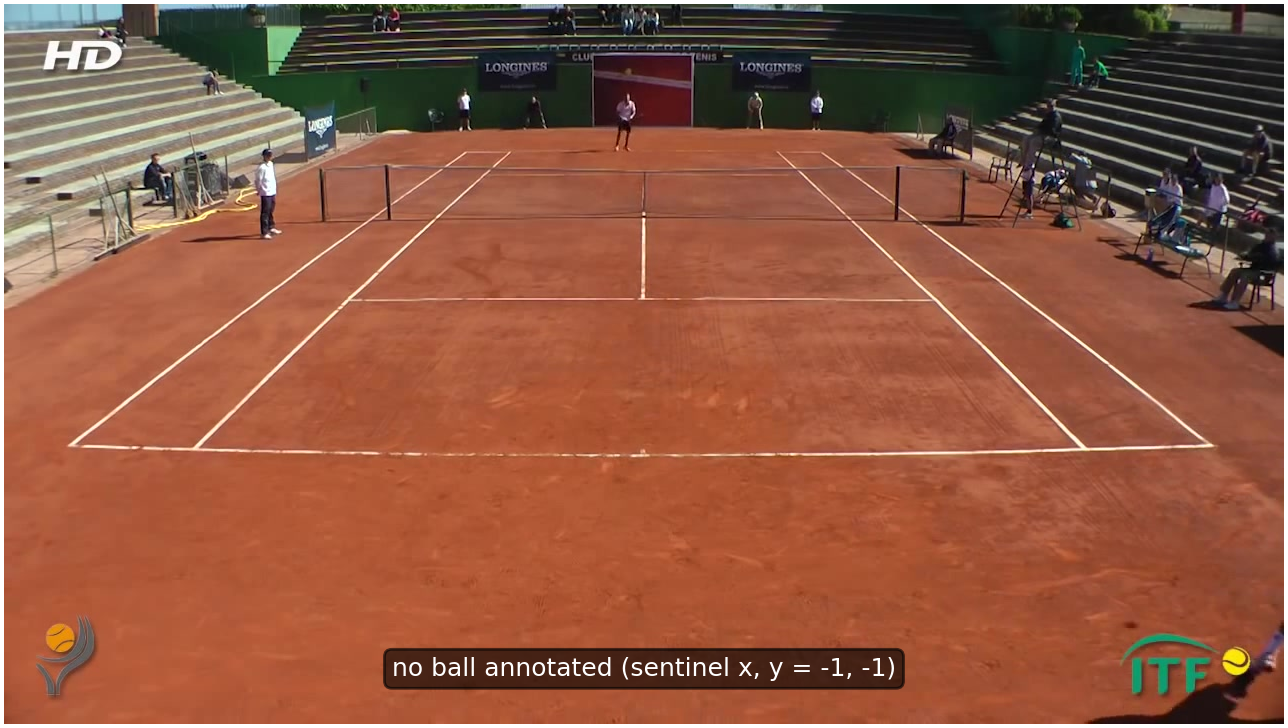
\includegraphics[width=\linewidth]{img/visibility_class0.png}
    \caption{Class 0: ball not visible}
  \end{subfigure}\hfill
  \begin{subfigure}{0.49\textwidth}
    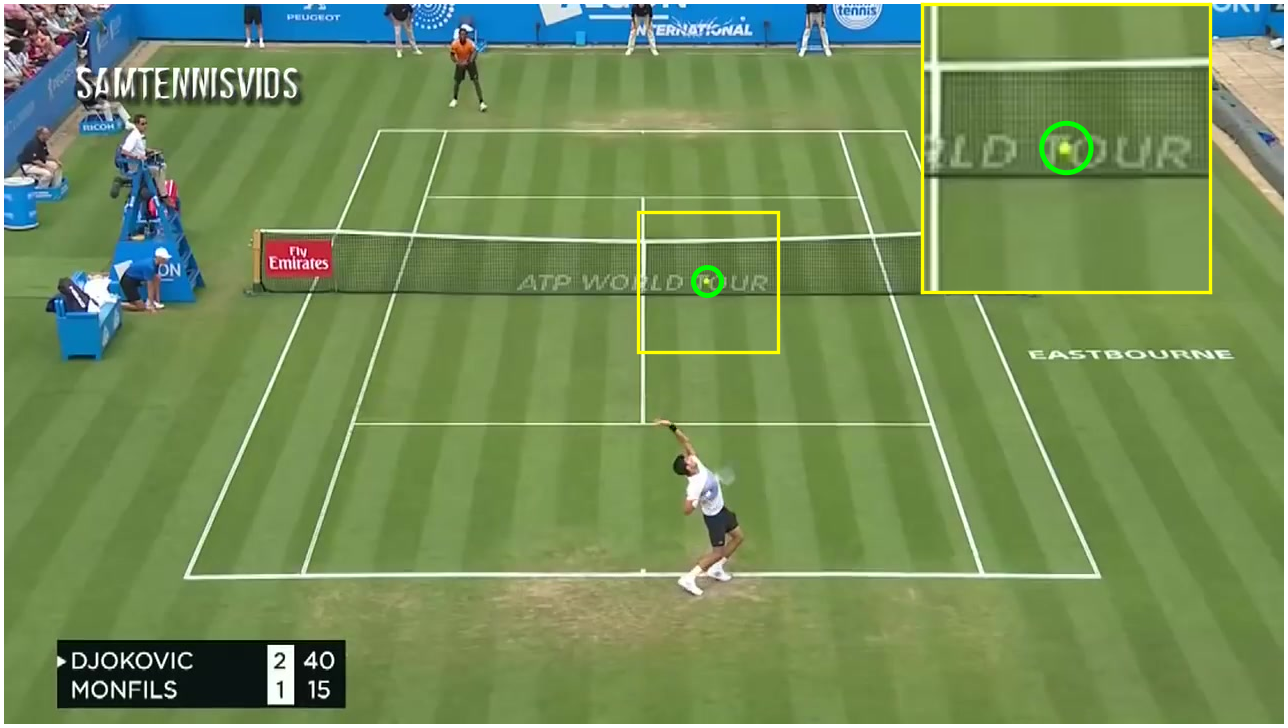
\includegraphics[width=\linewidth]{img/visibility_class1.png}
    \caption{Class 1: easily visible}
  \end{subfigure}

  \vspace{0.6em}
  \begin{subfigure}{0.49\textwidth}
    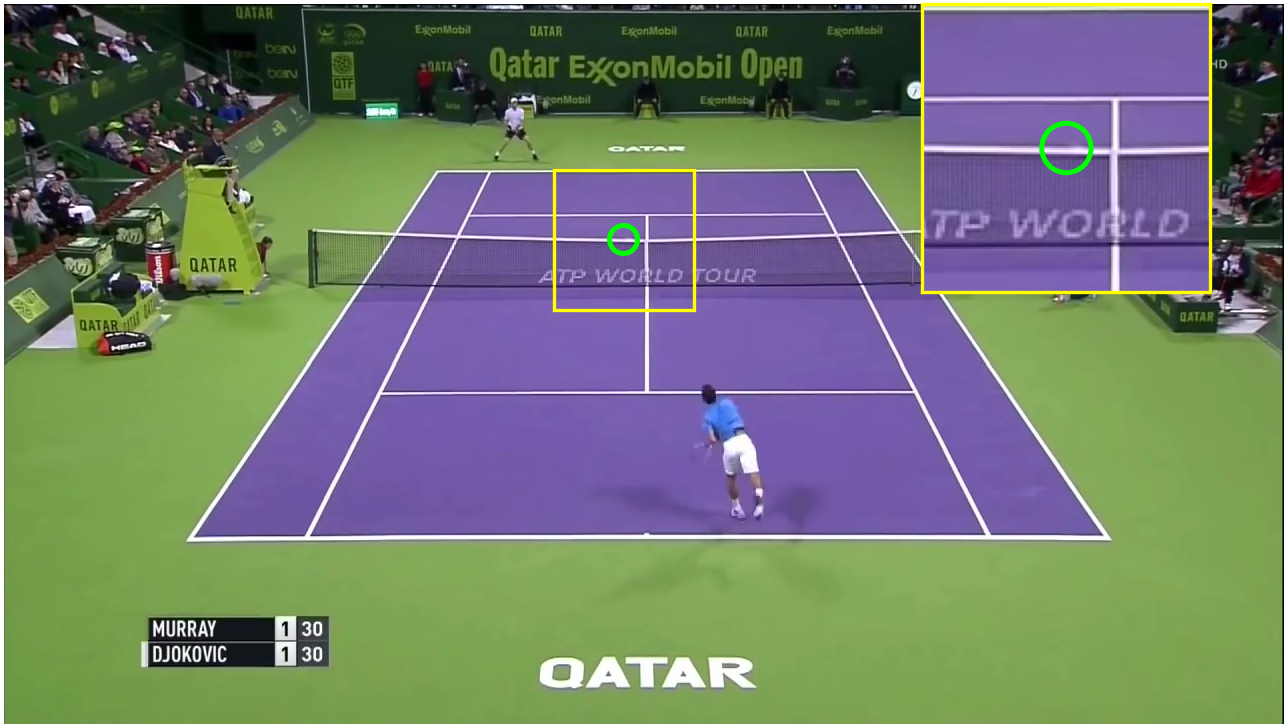
\includegraphics[width=\linewidth]{img/visibility_class2.png}
    \caption{Class 2: hard to identify}
  \end{subfigure}\hfill
  \begin{subfigure}{0.49\textwidth}
    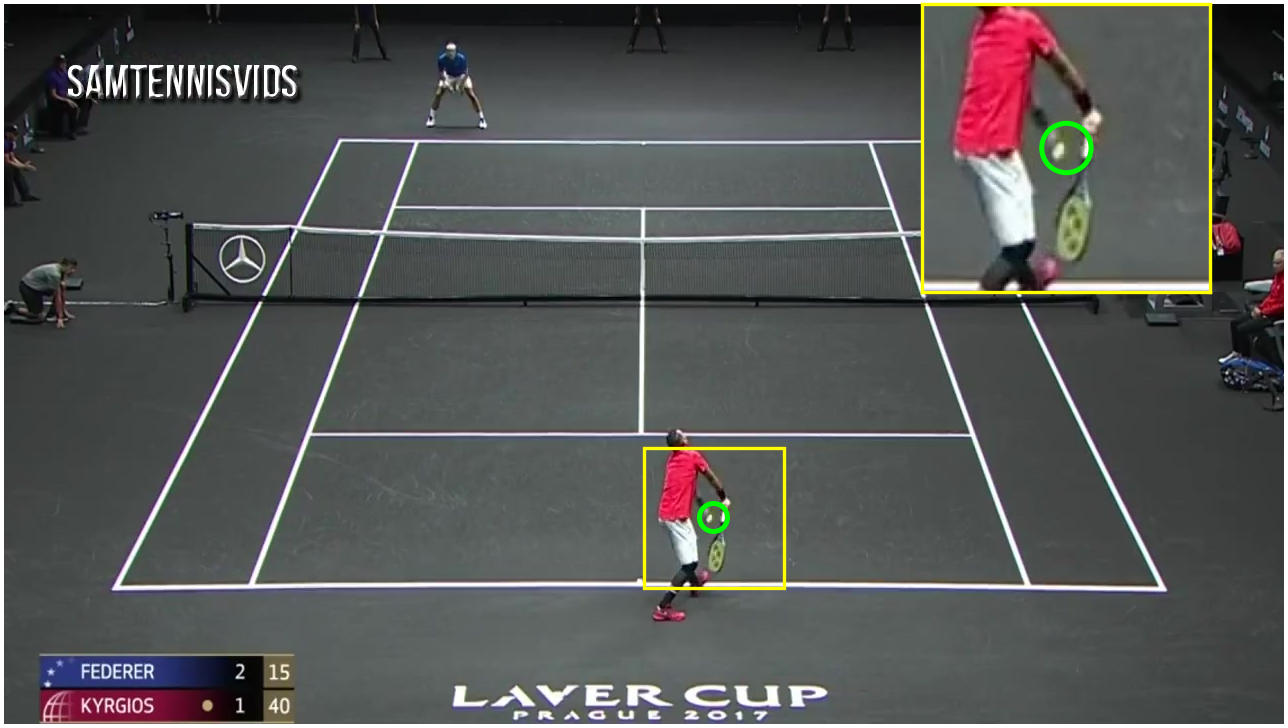
\includegraphics[width=\linewidth]{img/visibility_class3.png}
    \caption{Class 3: occluded}
  \end{subfigure}
  \caption{Representative frames for the four TrackNet visibility classes. In
    each panel the ground-truth ball position is marked with a green circle and
    magnified in the yellow inset; class~0 carries no ball annotation. The
    examples are drawn from different matches and court surfaces (clay, grass,
    and hard court), which also illustrates the visual variety of the dataset.}
  \label{fig:visibility-classes}
\end{figure}

Throughout the pipeline, a single encoding of the absence of a ball is used: when an
annotation carries visibility~0, or its coordinate fields are blank or negative,
the ball position is represented as $(-1, -1)$. This convention is preserved by
every dataset loader, model output, and metric in both the ball and bounce
projects, so that ``no ball'' is always distinguishable from a coordinate that
happens to lie near the image origin.

\begin{figure}[t]
  \centering
  \begin{subfigure}{0.32\textwidth}
    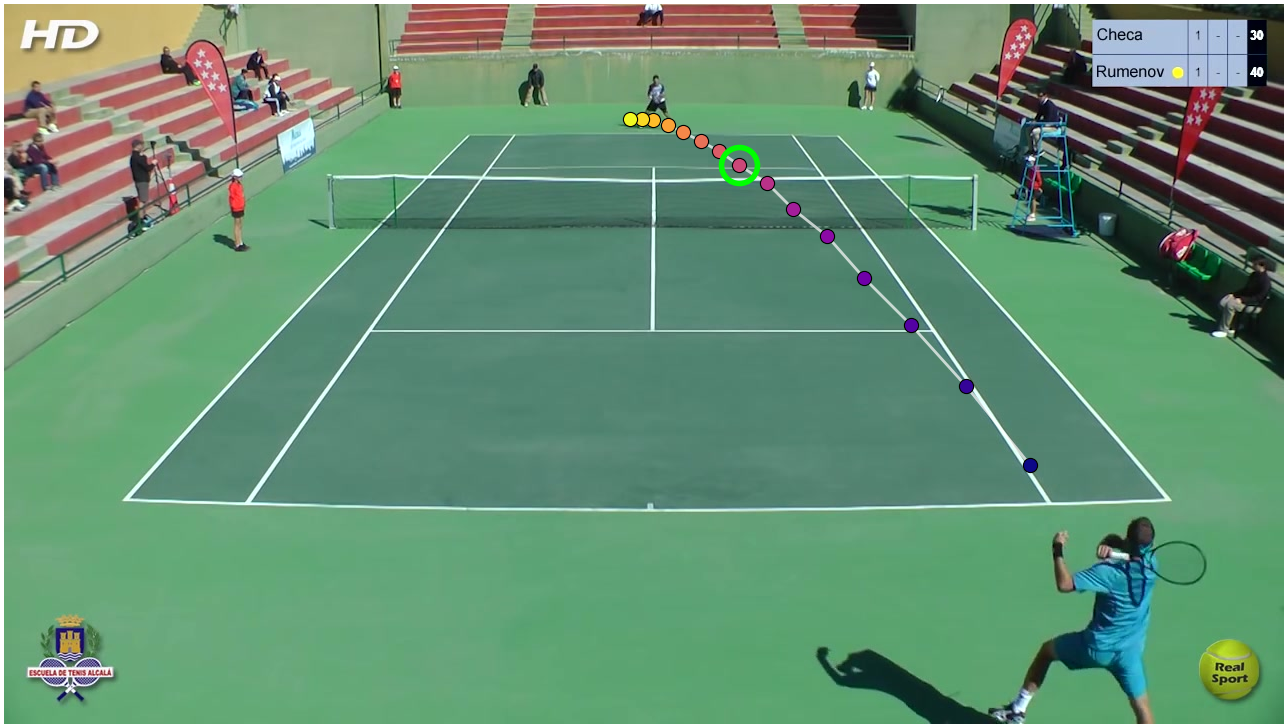
\includegraphics[width=\linewidth]{img/status_class0.png}
    \caption{Status 0: in flight}
  \end{subfigure}\hfill
  \begin{subfigure}{0.32\textwidth}
    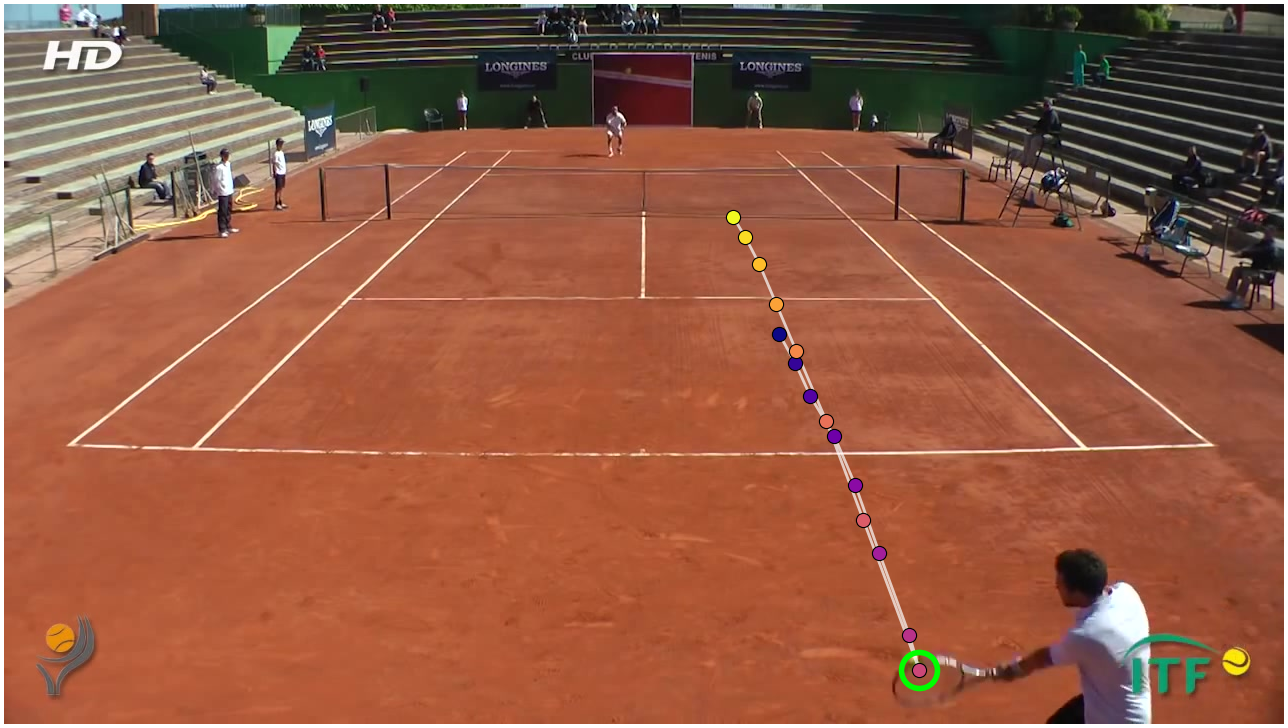
\includegraphics[width=\linewidth]{img/status_class1.png}
    \caption{Status 1: hit}
  \end{subfigure}\hfill
  \begin{subfigure}{0.32\textwidth}
    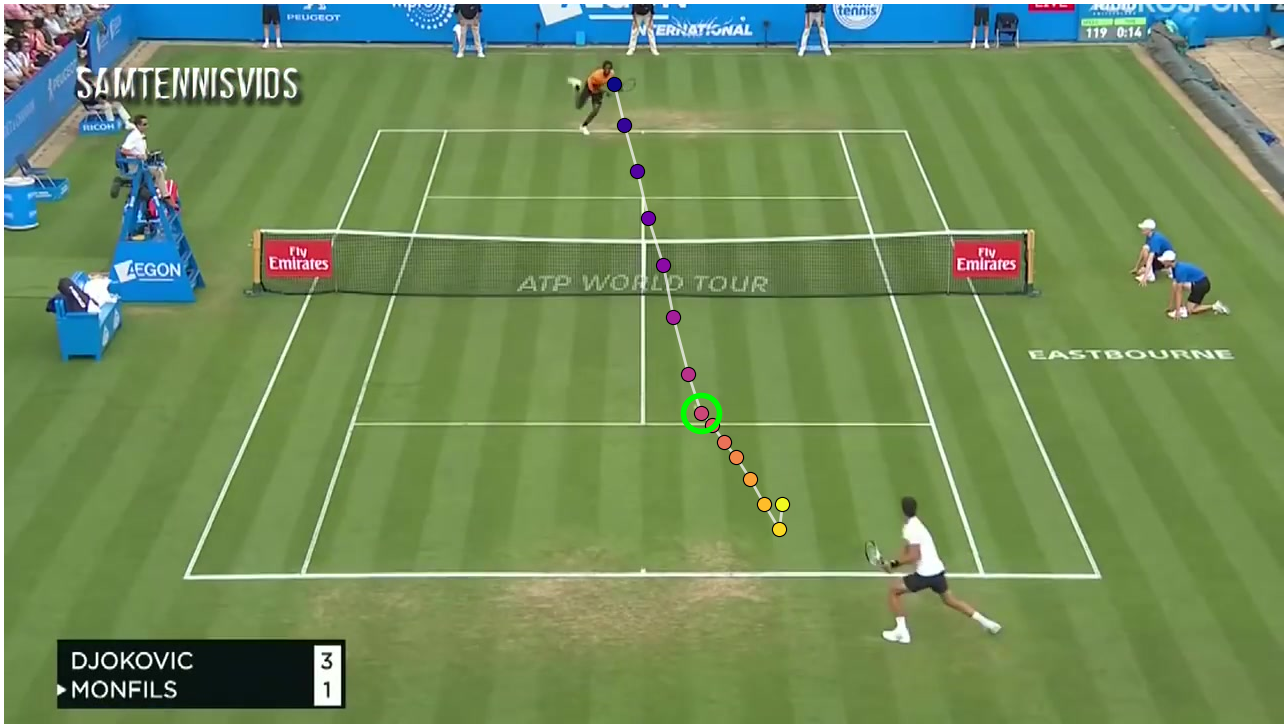
\includegraphics[width=\linewidth]{img/status_class2.png}
    \caption{Status 2: bounce}
  \end{subfigure}
  \caption{The three status values, each shown through the ball trajectory over
    a window of fifteen frames centred on an example event. Points are coloured
    by time (dark to bright), and the green ring marks the labelled frame. An
    in-flight frame lies on a smooth arc, a hit occurs where the ball is struck
    at the player's racket, and a bounce occurs where the ball lands on the
    court. These cues are temporal, which is why bounce detection
    (Chapter~\ref{ch:bounce}) operates on the trajectory rather than on single
    frames.}
  \label{fig:status-classes}
\end{figure}

\section{The Court-Keypoint Dataset}
\label{sec:meth-court}

Court keypoint detection is evaluated on a separate, publicly distributed
dataset, the TennisCourtDetector collection \cite{yastrebksv2023courtdetector},
which is unrelated to the TrackNet tennis data of
Section~\ref{sec:meth-tracknet}. It consists of 8{,}841 single RGB frames at an
original resolution of $1280 \times 720$ pixels, supplied as
``images/\{record\_id\}.png'', together with two JSON annotation files:
``data\_train.json'' with 6{,}630 records and ``data\_val.json'' with
2{,}211 records. Each record provides an identifier and a list of fourteen $[x, y]$ keypoints marking fixed court landmarks
such as the doubles and singles corners, the service points, and the centre
service-line intersections. Figure~\ref{fig:court-gt} shows two annotated frames
with these fourteen keypoints overlaid. The detailed ordering of these fourteen
keypoints, the construction of an inferred court-centre point from the
outer-court diagonals, and the canonical court template used for geometric
registration are specific to the court pipeline and are therefore deferred to
Chapter~\ref{ch:court}; only the dataset's overall size and split, needed to
define the protocol, are stated here.

\begin{figure}[t]
  \centering
  \begin{subfigure}{0.49\textwidth}
    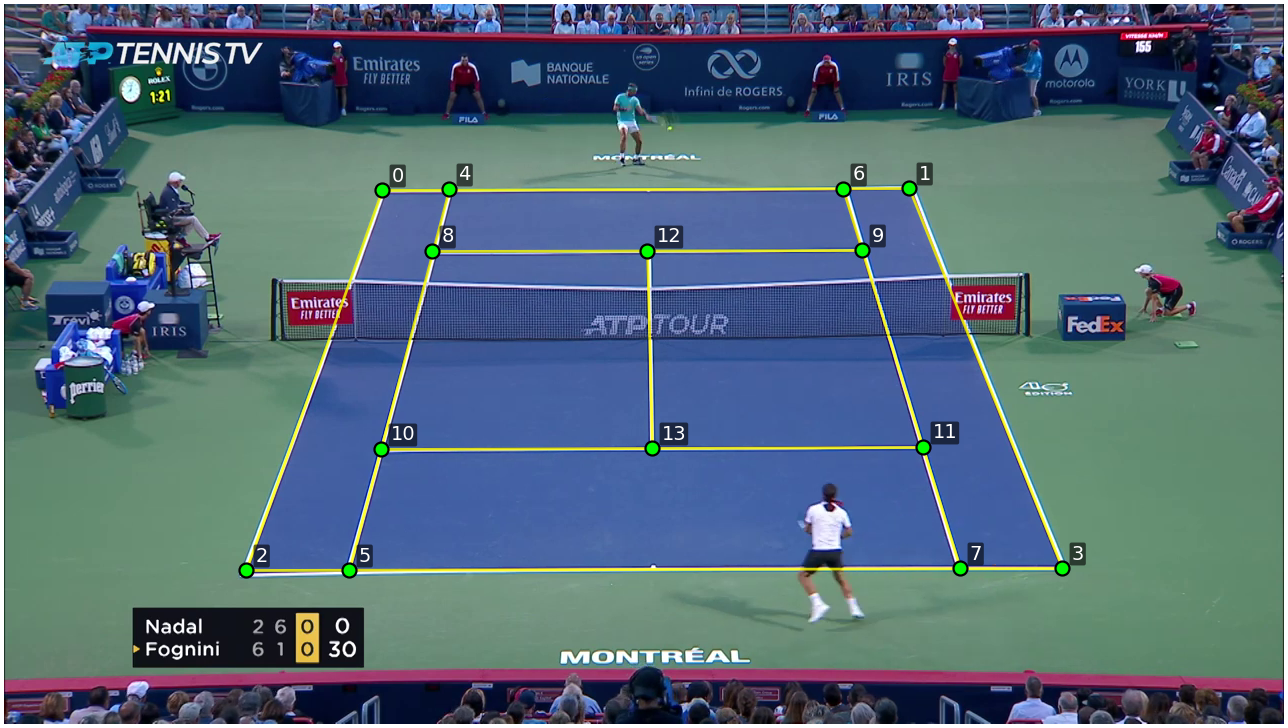
\includegraphics[width=\linewidth]{img/court_gt_example1.png}
    \caption{Hard court}
  \end{subfigure}\hfill
  \begin{subfigure}{0.49\textwidth}
    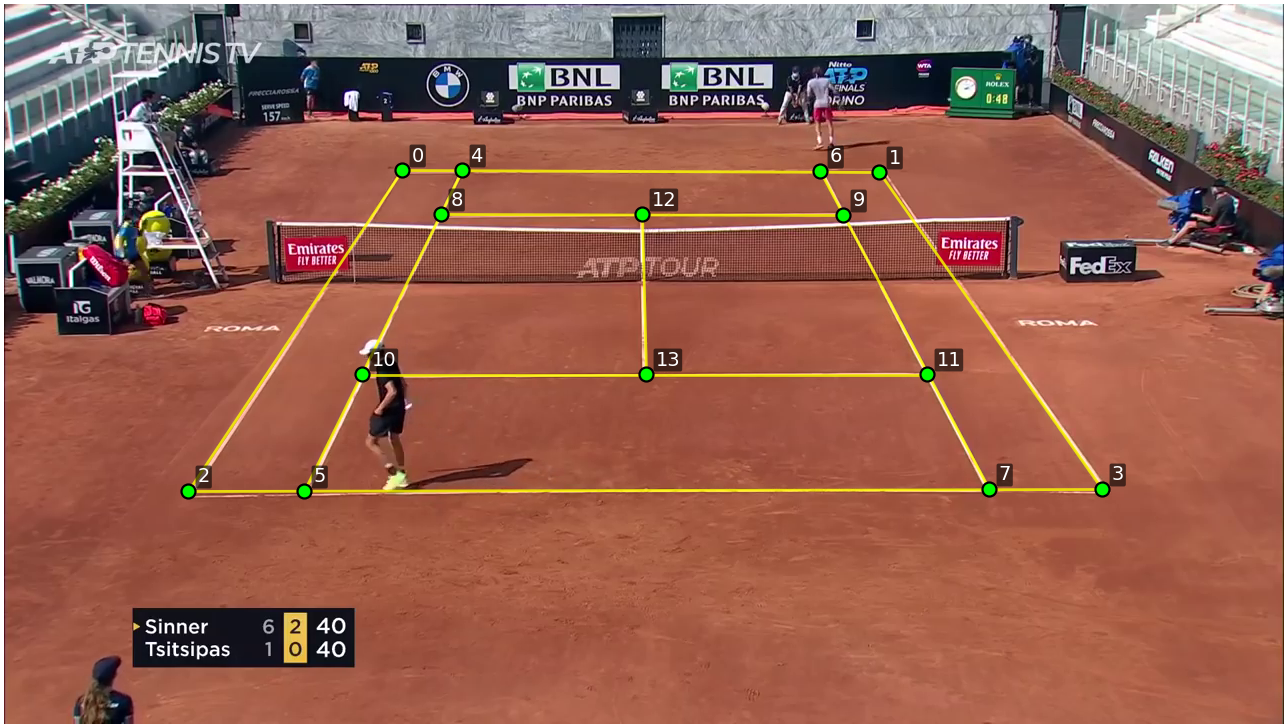
\includegraphics[width=\linewidth]{img/court_gt_example2.png}
    \caption{Clay court}
  \end{subfigure}
  \caption{Two example frames from the court-keypoint dataset with their
    ground-truth annotation overlaid. The fourteen annotated keypoints are shown
    as green markers numbered in the dataset ordering, and the yellow lines are
    the court boundaries they imply. The two frames show different camera angles
    and court surfaces, illustrating the variation the court models must handle.
    The meaning of each keypoint index is given in Chapter~\ref{ch:court}.}
  \label{fig:court-gt}
\end{figure}

\section{Non-Comparability of the Two Datasets}
\label{sec:meth-noncompare}

A point of method that recurs throughout the thesis is stated here once for
clarity. Ball tracking and bounce detection operate on the TrackNet tennis
dataset, whereas court detection operates on the TennisCourtDetector dataset.
The two differ in their content (a small moving ball against broadcast
backgrounds versus static court geometry), in their image resolution and source,
in their annotation schema (per-frame CSV labels versus per-image JSON
keypoints), and in their split policies (Section~\ref{sec:meth-splits}). Because
of these differences, accuracy figures are meaningful only within a
sub-task and must never be compared across sub-tasks. A pixel-accuracy
figure for the ball and a pixel-accuracy figure for court keypoints, for
instance, are measured on different images at different resolutions and do not
constitute a like-for-like comparison. The benchmark of this thesis is therefore
unified within each sub-task rather than across the three.

\section{Split Policies}
\label{sec:meth-splits}

All evaluation in this thesis rests on fixed, deterministic train, validation,
and test splits, so that every model within a sub-task is trained and judged on
exactly the same frames and the results are reproducible from a recorded seed.
The two datasets follow distinct split contracts, which are described in turn
and summarised together in Table~\ref{tab:splits}.

\subsection{TrackNet splits for ball and bounce}
\label{sec:meth-splits-tracknet}

Both TrackNet-based sub-tasks split the data by clip rather than by
frame, so that frames from one clip never appear in more than one split. This is
essential: consecutive frames within a clip are highly correlated, and allowing
them to straddle the train and test boundaries would leak information and inflate
the apparent accuracy. Within this shared principle, however, the two sub-tasks
adopt different partitions of the same 19{,}835-frame pool, reflecting their
different goals.

For ball tracking, matches game1 through game9 are used for
training and validation, and game10 is held out in its entirety as an
unseen test match. Within the training matches, the clips of each match are
shuffled with a fixed seed (42) and partitioned into 85\% training and 15\%
validation. This yields 14{,}812 training frames in 73 clips, 2{,}879
validation frames in 10 clips, and 2{,}144 test frames in 12 clips.

For bounce detection, a separate manifest holds out a different match,
game7, as the test set, because the goal is to measure event timing on a
match whose bounce patterns were never seen in training. The remaining matches
are partitioned into training and validation clips stratified by bounce density,
so that the scarce bounce events are represented in both partitions. This yields
14{,}697 training frames in 71 clips (387 bounce events), 3{,}257 validation
frames in 15 clips (86 bounce events), and 1{,}881 test frames in 9 clips (50
bounce events).

The consequence, made explicit in Table~\ref{tab:splits}, is that even the two
TrackNet sub-tasks draw their test sets from different matches
(game10 for the ball, game7 for bounces) and partition the
remaining data by different rules. Their figures are therefore reported against
different held-out data and are not interchangeable, a finer instance of the
non-comparability principle of Section~\ref{sec:meth-noncompare}.

\subsection{Court split}
\label{sec:meth-splits-court}

The court-keypoint dataset is split deterministically without a random seed.
The 6{,}630 records of ``data\_train.json'' are used as the training set
as supplied. The 2{,}211 records of ``data\_val.json'' are ordered by the MD5 hash of their
record identifier and divided in half: the first 1{,}105
records form the validation set and the remaining records form the test set.
Six test records carrying semantically incorrect annotations are excluded,
leaving 1{,}100 test records.

\begin{table}[h]
  \centering
  \small
  \caption{Split allocations for the three sub-tasks. The two TrackNet sub-tasks
    (ball, bounce) share the same 19{,}835-frame pool but use different held-out
    test matches and different partition rules; the court sub-task uses a
    separate dataset of image records, so its counts are not comparable with the
    TrackNet columns.}
  \label{tab:splits}
  \begin{tabular}{l rr rrr r}
    \toprule
    & \multicolumn{2}{c}{Ball (TrackNet)} & \multicolumn{3}{c}{Bounce (TrackNet)} & Court \\
    \cmidrule(lr){2-3} \cmidrule(lr){4-6} \cmidrule(lr){7-7}
    Split & Frames & Clips & Frames & Clips & Bounces & Records \\
    \midrule
    Train & 14{,}812 & 73 & 14{,}697 & 71 & 387 & 6{,}630 \\
    Val   &  2{,}879 & 10 &  3{,}257 & 15 &  86 & 1{,}105 \\
    Test  &  2{,}144 & 12 &  1{,}881 &  9 &  50 & 1{,}100 \\
    \midrule
    Total & 19{,}835 & 95 & 19{,}835 & 95 & 523 & 8{,}835 \\
    \bottomrule
  \end{tabular}
\end{table}

\section{Shared Evaluation Philosophy and Metric Vocabulary}
\label{sec:meth-metrics}

The comparisons in this thesis are designed so that every model within a
sub-task is scored by an identical, fixed metric suite, computed by shared
evaluation code rather than re-implemented per model. This section defines each
metric once. Which metrics apply to which sub-task is itself task-specific, and
the actual measured values appear in the relevant results chapters. 

\subsection{Localisation metrics}
\label{sec:meth-metrics-loc}

Localisation accuracy, used for both the ball and the court keypoints, is built
on the Euclidean pixel distance between a prediction $\hat{p}_i$ and its
ground-truth position $p_i$,
\begin{equation}
  d_i = \lVert \hat{p}_i - p_i \rVert_2,
  \label{eq:pixdist}
\end{equation}
where both positions are expressed in the original-image pixel space. From this
distance two families of metric are derived.

The first is a thresholded accuracy: the fraction of visible targets whose
prediction falls within a tolerance $\tau$ pixels of the ground truth,
\begin{equation}
  \mathrm{acc@}\tau\mathrm{px} = \frac{1}{|\mathcal{V}|}\sum_{i \in \mathcal{V}}
  \mathbb{1}\!\left[ d_i \le \tau \right],
  \label{eq:accthr}
\end{equation}
where $\mathcal{V}$ is the set of ground-truth-visible targets and
$\mathbb{1}[\cdot]$ is the indicator function. For ball tracking this quantity
is reported at $\tau \in \{5, 10, 20\}$ and written $\mathrm{acc@}\tau$px; for
court keypoints the identical quantity is the percentage of correct keypoints,
written $\mathrm{PCK@}\tau$px, and reported at $\tau \in \{5, 7, 10, 25\}$ with
$\tau = 7$ used as the primary monitoring threshold during training.

The second family reports the mean error directly. The mean absolute error in
pixels, $\mathrm{MAE_{px}}$, is the average of $d_i$ over visible targets. For
ball tracking it is additionally broken down per visibility class (classes 1, 2,
and 3 of Section~\ref{sec:meth-tracknet-schema}; class~0 carries no ball and is
excluded), exposing how localisation degrades as the ball becomes harder to see.
For court keypoints the mean keypoint error is complemented by the median and
maximum keypoint error over detected points, which characterise the typical and
worst-case localisation respectively.

\subsection{Detection metrics}
\label{sec:meth-metrics-det}

Localisation accuracy presupposes that the target was found; detection metrics
measure whether it was found at all. For ball tracking, a binary
visibility decision (does the model report a ball, and is there in fact a ball?)
yields a precision, recall, and $F_1$ from the counts of true positives,
false positives, and false negatives. A stricter, location-aware variant,
following the convention of the TrackNet evaluation \cite{huang2019tracknet},
counts a prediction as a true positive only when the model reports a ball, the
ground truth contains a ball, and the predicted position lies within five pixels
of it; a reported ball that is absent in the ground truth or mislocated beyond
five pixels is a false positive, and a missed visible ball is a false negative.
This produces $\mathrm{precision@5px}$, $\mathrm{recall@5px}$, and
$\mathrm{F1@5px}$, which jointly penalise both missed detections and confident
mislocalisations.
\subsection{Event metrics}
\label{sec:meth-metrics-event}

Bounce detection is scored as an event-timing problem rather than a per-frame
classification problem. Because bounce frames make up under 3\% of the data
(Table~\ref{tab:tracknet-labels}), a per-frame accuracy would be dominated by
the negative class and is deliberately not reported. Instead, each model emits a
per-frame bounce score; this signal is decoded into discrete event
predictions by locating its peaks subject to a minimum spacing between
successive events, and the predicted events are matched to ground-truth
bounces by greedy one-to-one assignment within a temporal tolerance of
$\pm k$ frames. From the resulting true positives, false positives, and false
negatives, an event precision, recall, and $F_1$ at tolerance $k$ are computed
via Equation~\eqref{eq:f1}; the default tolerance is $k = 3$ frames. Two further
summaries characterise behaviour beyond a single operating point: the average
precision (AP), obtained as the area under the precision-recall curve traced by
sweeping the decode threshold, and a tolerance sweep that reports $F_1$ at
$k \in \{0, 1, 2, 3, 5, 7\}$ to show how timing accuracy tightens or relaxes the
score. A bounce-versus-hit confusion count, which buckets each predicted bounce
according to whether the nearest ground-truth event within the tolerance window
is a bounce, a hit, or neither, quantifies the extent to which racket hits are
mistaken for bounces. It should be noted that AP and $F_1$ at a tolerance are
different quantities at different operating points and are not interchangeable; a
comparison between them is made only at a fixed tolerance, never as a single
headline gap.

\subsection{Geometric and efficiency metrics}
\label{sec:meth-metrics-geom}

For the court sub-task, keypoint accuracy is supplemented by metrics that
measure the quality of the downstream geometric registration. A homography is
estimated from the predicted keypoints, the visible ground-truth keypoints are
projected through it into the canonical court plane, and their displacement from
the template is reported in centimetres as a mean and a maximum reprojection
error, alongside the rate at which a homography could be estimated at all. The
estimation procedure itself, including its robust fitting and the canonical
court template, is described where it is used, in Chapter~\ref{ch:court}.

Finally, efficiency is reported uniformly across all sub-tasks through two
quantities: the inference throughput in frames per second (FPS), and the model
size as a parameter count in millions. These allow the accuracy of each model to
be read against its computational cost, which is key idea to the accuracy-versus-
speed trade-offs examined in the results chapters and to the model-selection
rationale of the integrated system (Chapter~\ref{ch:integrated}).

With the datasets, split contracts, and metric definitions now fixed, the
following three chapters apply this protocol in turn: ball tracking in
Chapter~\ref{ch:ball}, court keypoint detection and homography in
Chapter~\ref{ch:court}, and bounce-event detection in Chapter~\ref{ch:bounce}.
Each of those chapters also describes the training details specific to its
models, including the optimiser, loss function, and hyperparameters.

\chapter{Ball Tracking}
\label{ch:ball}

% Compact node styles for the TrackNet-family architecture schematics (Fig.~\ref{fig:ball-arch}).
\tikzset{
  tn/.style={rectangle, draw=blue!55, fill=blue!5, rounded corners,
    align=center, minimum height=0.85cm, text width=1.7cm,
    font=\scriptsize\sffamily, semithick},
  tnio/.style={tn, draw=gray!65, fill=gray!12},
  tnmod/.style={tn, draw=orange!80, fill=orange!15},
  tnarr/.style={-{Stealth[scale=0.9]}, line width=0.6pt, gray!70},
}

This chapter applies the protocol of Chapter~\ref{ch:methodology} to the first
and most demanding perception sub-task of the system, localising the tennis
ball in every frame. The ball is small, often blurred by its own speed, and
regularly hidden by players, the net, or the court markings, so its position
must be inferred from motion across several frames rather than from any single
image. Six models are compared: the five published members of the TrackNet
family, V1 through V5, and a single-frame object detector, YOLO11m, included as
a representative of the bounding-box paradigm against which the heatmap
formulation is contrasted. All six operate on the TrackNet tennis dataset
described in Section~\ref{sec:meth-tracknet} and are scored by the localisation
and detection metrics of Sections~\ref{sec:meth-metrics-loc}
and~\ref{sec:meth-metrics-det}.

The comparison follows a deliberate two-stage selection protocol, which shapes
how the results in Sections~\ref{sec:ball-selection}
and~\ref{sec:ball-final} should be read. In the first stage, architecture
selection, all six models were trained and evaluated on a smaller subset split
in order to compare the architectures cheaply. In the second stage, the single
winner of that comparison, TrackNetV4, was retrained on the full dataset split
defined in Section~\ref{sec:meth-splits-tracknet}. The two stages therefore
report different numbers measured on different held-out matches, and a figure
from one stage is never placed beside a figure from the other without that
distinction being made explicit. This design is a defensible compromise between
rigour and cost: it compares six architectures on a common footing, then
invests full-dataset training only in the chosen one, and it is the structure
through which the chapter answers the first research question (RQ1) on which
architecture best localises the ball and what the architectural progression
buys in accuracy against speed.

\section{Task Formulation}
\label{sec:ball-task}

Ball tracking is posed here as per-frame localisation rather than as
multi-object tracking. For each frame the model must report either a single
image coordinate for the ball or an explicit indication that no ball is
present, and the per-frame outputs are read as a trajectory without an explicit
data-association stage. Two formulations of this task are compared. In the
heatmap formulation, which the TrackNet family adopts, the network predicts a
spatial response map whose peak marks the ball centre, and the coordinate is
recovered by locating the maximum response; the absence of a ball is expressed
naturally as a map with no significant peak \cite{huang2019tracknet,
zhou2019centernet}. In the bounding-box formulation, which the YOLO detector
adopts, the network regresses a box around the ball and its centre is taken as
the position, with a confidence score gating whether a ball is reported at all
\cite{redmon2016yolo}. The contrast between these two formulations on a small,
fast, frequently occluded target is the central question of the chapter, and
the absence of a ball is represented throughout by the coordinate $(-1, -1)$,
the sentinel defined in Section~\ref{sec:meth-tracknet}.

\section{Preprocessing and Learning Targets}
\label{sec:ball-preproc}

The temporal cue that distinguishes a moving ball from the static background is
provided to the models by stacking consecutive frames. For the TrackNet family
a sliding window of three consecutive frames is read from a clip and stacked
along the channel axis into a nine-channel input, with the ball position of the
middle frame as the target; the first and last frames of every clip are skipped
so that a complete window of three frames is always available. The frames are
resized before stacking, and the resize convention differs by model and by
stage. In the architecture-selection comparison of
Section~\ref{sec:ball-selection}, V1, V4, and V5 operate on a square
$256 \times 256$ input, V2 and V3 at $512 \times 288$, and the YOLO detector at
its native $640 \times 640$; the final TrackNetV4 of
Section~\ref{sec:ball-final} was retrained at the higher $640 \times 368$
resolution, which preserves the broadcast aspect ratio rather than squashing it
to a square. These conventions are not
intermixed, and every coordinate reported by a model is both expressed and
scored in its own resized pixel space rather than being rescaled to a common
frame.

The learning target depends on how each model represents the ball. The original
V1 design and its V4 descendant do not regress a continuous heatmap but instead
predict a quantised intensity class map: a Gaussian centred on the ball, of
half-size 20 pixels and variance 10, is rendered and quantised so that each
pixel carries an integer intensity class in the range $[0, 255]$, with the peak
value 255 at the ball centre, and the network is trained to classify every
pixel into one of these 256 classes. V2 and V3 instead regress a continuous
Gaussian heatmap with a sigmoid output and a peak value of one, as does V5. The
YOLO detector is trained against a fixed bounding box of 20 pixels placed around
the labelled point, in the YOLO annotation format. In all cases a frame whose
ball is invisible (visibility class~0, or a blank or negative coordinate)
produces an all-zero target and contributes the $(-1, -1)$ sentinel rather than
a spurious position.

Data augmentation is applied to the training split only, with validation and
test frames left unaltered. The augmentation perturbs brightness by up to
$\pm 0.3$ of the intensity range and scales contrast by a factor drawn from
$[0.7, 1.3]$, and with probability one half it flips the frame window
horizontally. The flip is the one augmentation that interacts with the label:
when a window is flipped, the ball x-coordinate is remapped to $W - 1 - x$,
where $W$ is the frame width, so that the target stays aligned with the
image, while an invisible ball (coordinate $-1$) is left untouched. The same
transformation is applied consistently across all three frames of a window so
that the temporal cue is preserved.

\section{Models}
\label{sec:ball-models}

The five TrackNet variants share a common lineage, an encoder-decoder
convolutional network with skip connections that ingests the nine-channel frame
stack and produces a spatial output at the input resolution
\cite{huang2019tracknet}. They differ in the output representation, in the depth
of the encoder-decoder, and in the temporal-reasoning module each one adds.
Table~\ref{tab:ball-models} summarises the six models along the axes that
matter for the comparison, and the architecture of each of the five TrackNet
variants is drawn in Figure~\ref{fig:ball-arch}, panels (a) to (e).

\begin{table}[t]
  \centering
  \small
  \setlength{\tabcolsep}{4pt}
  \caption{The six ball-tracking models compared in this chapter. The TrackNet
    family shares an encoder-decoder backbone and differs in its output
    representation and temporal module; YOLO11m is a single-frame bounding-box
    detector included as the non-heatmap baseline. Parameter counts are computed
    from the implementations used here; the YOLO11m figure is the published size
    of the Ultralytics medium model \cite{jocher2024yolo11}.}
  \label{tab:ball-models}
  \begin{tabular}{@{}l >{\raggedright\arraybackslash}p{3.0cm} >{\raggedright\arraybackslash}p{4.8cm} r@{}}
    \toprule
    Model & Output target  & Distinctive module & \makecell[r]{Params\\(M)} \\
    \midrule
    TrackNet (V1) & 256-class intensity map  & VGG encoder-decoder & 20.9 \\
    TrackNetV2    & multi-frame heatmaps      & multiple-in multiple-out & 11.3 \\
    TrackNetV3    & multi-frame heatmaps      & median background + InpaintNet & 11.3 \\
    TrackNetV4    & 256-class intensity map & motion-attention gating & 20.9 \\
    TrackNetV5    & single heatmap          & temporal self-attention & 21.9 \\
    YOLO11m       & bounding box            & anchor-free box regression & 20.1 \\
    \bottomrule
  \end{tabular}
\end{table}

TrackNet (V1), in panel~(a), follows the original design
\cite{huang2019tracknet}: a
four-stage VGG-style encoder with max-pooling, a convolutional bottleneck, and a
symmetric decoder whose transposed convolutions are concatenated with the
matching encoder features through skip connections. A final $1 \times 1$
convolution maps the decoded features to 256 channels, one per intensity class,
and the position is recovered by taking the per-pixel argmax to form an
intensity image and locating its global peak; a peak below an intensity
threshold yields the no-ball sentinel. This is a multiple-in single-out design,
three frames in and one ball position out.

TrackNetV2, in panel~(b), reorganises the backbone into a multiple-in
multiple-out form that predicts a sigmoid Gaussian heatmap for every frame in
the window in a single pass, reducing redundant computation
\cite{sun2020tracknetv2}. Its
encoder-decoder is shallower than V1's, three stages rather than four, with
nearest-neighbour upsampling in the decoder, which roughly halves the parameter
count to 11.3~million. The coordinate is the argmax of the relevant frame's
heatmap when its peak exceeds 0.5, and the sentinel otherwise.

TrackNetV3, in panel~(c), builds on the V2 backbone with two additions
aimed at robustness \cite{chen2023tracknetv3}. A per-pixel median-background channel,
computed across the input window, is concatenated to the frame stack so that the
network sees an explicit estimate of the static scene. Separately, an
inpainting network, a small one-dimensional U-Net that takes a sequence of
predicted coordinates with a visibility flag and outputs a rectified sequence,
repairs missed detections by reasoning over the predicted path; it is trained
with a mean-squared-error objective on the trajectory and operates as a
post-processing stage over the tracker's per-frame peaks.

TrackNetV4, in panel~(d), is the model selected in
Section~\ref{sec:ball-selection}. It keeps the V1 backbone and
256-class output, and adds a lightweight motion-attention module
\cite{raj2025tracknetv4}. The module forms absolute differences between
successive input frames, passes the concatenated difference maps through two
convolutions and a sigmoid to produce a single-channel spatial attention map,
and multiplies this map into the decoder features at two resolutions. The effect
is to amplify regions of recent motion, where a fast ball is likely to be, while
suppressing the static background, at a negligible parameter cost over V1
(20.9~million for both).

TrackNetV5, in panel~(e), encodes each of the three frames independently
with a shared
VGG-style encoder, then fuses their deepest features with a multi-head temporal
self-attention layer that treats the three frames as a short sequence at each
spatial position, before decoding from the attended middle-frame features to a
single sigmoid heatmap. It is the largest of the family at 21.9~million
parameters. As noted in Section~\ref{sec:rw-tracknet}, V5 is a preprint variant
\cite{tang2025tracknetv5} and is included to test whether learned temporal
attention improves on the explicit motion cue of V4.

YOLO11m is a single-frame, anchor-free object detector from the
Ultralytics YOLO family \cite{jocher2024yolo11, redmon2016yolo}. Unlike the
TrackNet models it sees one frame at a time and regresses a bounding box whose
centre is taken as the ball position, with a confidence threshold of 0.3 below
which no ball is reported. It carries no temporal cue and serves as the
bounding-box baseline against which the heatmap formulation is measured.

\begin{figure}[p]
  \centering
  \begin{subfigure}{\textwidth}
    \centering
    \resizebox{\textwidth}{!}{%
    \begin{tikzpicture}[node distance=0.4cm and 0.6cm]
      \node[tnio] (i) {3 frames\\(9 ch)};
      \node[tn, right=of i] (e) {encoder\\4 stages};
      \node[tn, right=of e] (b) {bottleneck};
      \node[tn, right=of b] (d) {decoder\\+ skips};
      \node[tn, right=of d] (h) {256-class\\head};
      \node[tnio, right=of h] (o) {$\arg\max$\\$\to (x,y)$};
      \foreach \x/\y in {i/e,e/b,b/d,d/h,h/o} \draw[tnarr] (\x) -- (\y);
    \end{tikzpicture}}
    \caption{TrackNet (V1): four-stage VGG encoder-decoder with skip
      connections and a 256-class intensity head; multiple-in, single-out.}
    \label{fig:arch-v1}
  \end{subfigure}

  \vspace{0.8em}
  \begin{subfigure}{\textwidth}
    \centering
    \resizebox{\textwidth}{!}{%
    \begin{tikzpicture}[node distance=0.4cm and 0.6cm]
      \node[tnio] (i) {3 frames\\(9 ch)};
      \node[tn, right=of i] (e) {encoder\\3 stages};
      \node[tn, right=of e] (b) {bottleneck};
      \node[tn, right=of b] (d) {decoder\\+ skips\\(NN up)};
      \node[tn, right=of d] (h) {3 heatmaps\\(MIMO)};
      \node[tnio, right=of h] (o) {$\arg\max$\\$\to (x,y)$};
      \foreach \x/\y in {i/e,e/b,b/d,d/h,h/o} \draw[tnarr] (\x) -- (\y);
    \end{tikzpicture}}
    \caption{TrackNetV2: shallower three-stage backbone that emits one heatmap
      per input frame in a single multiple-in multiple-out pass.}
    \label{fig:arch-v2}
  \end{subfigure}

  \vspace{0.8em}
  \begin{subfigure}{\textwidth}
    \centering
    \resizebox{\textwidth}{!}{%
    \begin{tikzpicture}[node distance=0.4cm and 0.6cm]
      \node[tnio] (i) {frames +\\median bg\\(27 ch)};
      \node[tn, right=of i] (bb) {V2 backbone\\(MIMO)};
      \node[tn, right=of bb] (hm) {per-frame\\heatmaps};
      \node[tn, right=of hm] (p) {peak\\coords};
      \node[tnmod, right=of p] (ip) {InpaintNet\\1D U-Net};
      \node[tnio, right=of ip] (o) {rectified\\trajectory};
      \foreach \x/\y in {i/bb,bb/hm,hm/p,p/ip,ip/o} \draw[tnarr] (\x) -- (\y);
    \end{tikzpicture}}
    \caption{TrackNetV3: the V2 tracker fed an extra median-background channel,
      followed by an InpaintNet that rectifies the trajectory (shaded).}
    \label{fig:arch-v3}
  \end{subfigure}

  \vspace{0.8em}
  \begin{subfigure}{\textwidth}
    \centering
    \resizebox{\textwidth}{!}{%
    \begin{tikzpicture}[node distance=0.5cm and 0.6cm]
      \node[tnio] (i) {3 frames\\(9 ch)};
      \node[tn, right=of i] (e) {encoder};
      \node[tn, right=of e] (b) {bottleneck};
      \node[tn, right=of b] (d) {decoder\\+ skips};
      \node[tn, right=of d] (h) {256-class\\head};
      \node[tnio, right=of h] (o) {$\arg\max$\\$\to (x,y)$};
      \node[tnmod, below=0.7cm of b] (m) {motion\\attention};
      \foreach \x/\y in {i/e,e/b,b/d,d/h,h/o} \draw[tnarr] (\x) -- (\y);
      \draw[tnarr] (i.south) |- (m.west);
      \draw[tnarr] (m.east) -| (d.south);
    \end{tikzpicture}}
    \caption{TrackNetV4: the V1 backbone with a motion-attention branch (shaded)
      that gates the decoder towards moving regions; the selected model.}
    \label{fig:arch-v4}
  \end{subfigure}

  \vspace{0.8em}
  \begin{subfigure}{\textwidth}
    \centering
    \resizebox{\textwidth}{!}{%
    \begin{tikzpicture}[node distance=0.4cm and 0.55cm]
      \node[tnio] (i) {3 frames\\(per frame)};
      \node[tn, right=of i] (e) {shared\\encoder};
      \node[tn, right=of e] (b) {bottleneck\\feats $\times 3$};
      \node[tnmod, right=of b] (a) {temporal\\self-attn.};
      \node[tn, right=of a] (d) {decode\\middle};
      \node[tn, right=of d] (h) {heatmap};
      \node[tnio, right=of h] (o) {$\arg\max$\\$\to (x,y)$};
      \foreach \x/\y in {i/e,e/b,b/a,a/d,d/h,h/o} \draw[tnarr] (\x) -- (\y);
    \end{tikzpicture}}
    \caption{TrackNetV5: each frame is encoded independently and the three
      bottleneck features are fused by temporal self-attention (shaded) before
      decoding the middle frame.}
    \label{fig:arch-v5}
  \end{subfigure}

  \caption{Architecture of the five TrackNet-family variants compared in this
    chapter. All share an encoder-decoder backbone that ingests stacked frames
    and produces a spatial output decoded to a ball coordinate; they differ in
    the output representation and in the temporal module each one adds, shaded
    for the trajectory rectifier of V3, the motion attention of V4, and the
    temporal self-attention of V5.}
  \label{fig:ball-arch}
\end{figure}

\section{Training Details}
\label{sec:ball-training}

All models were trained on a single GPU with a learning-rate schedule that
reduced the rate by half when the validation loss plateaued, and with early
stopping that halted training when the validation accuracy at five pixels failed
to improve for a fixed number of epochs. Within this common regime the models
differ in optimiser, loss, and the hyperparameters listed in
Table~\ref{tab:ball-train}. The two 256-class models, V1 and V4, were trained
with the Adadelta optimiser and a cross-entropy loss over the intensity classes;
the heatmap-regressing V2 and V3 trackers used the Adam optimiser
\cite{kingma2015adam} with a weighted binary cross-entropy that emphasises the
sparse positive pixels in the manner of focal loss \cite{lin2017focalloss}; V5
used Adam with a plain binary cross-entropy on its sigmoid heatmap; and the
InpaintNet rectifier of V3 was trained separately with mean-squared error on the
coordinate sequence. YOLO11m was trained through the Ultralytics framework with
its own composite detection loss and optimiser defaults. The differences in
batch size and epoch budget in Table~\ref{tab:ball-train} reflect the differing
memory footprints and convergence behaviour of the models rather than a tuned
search, and every model was trained under the identical subset split of
Section~\ref{sec:ball-selection} so that the comparison is like-for-like.

\begin{table}[t]
  \centering
  \small
  \setlength{\tabcolsep}{6pt}
  \caption{Training configuration of the six models. All used a
    reduce-on-plateau learning-rate schedule and early stopping; they differ in
    optimiser, loss, and budget. The two 256-class models (V1, V4) use Adadelta
    with cross-entropy; the heatmap models use Adam.}
  \label{tab:ball-train}
  \begin{tabular}{l l l r r r}
    \toprule
    Model & Optimiser & Loss & \makecell[r]{Init.\\LR} & Batch & Epochs \\
    \midrule
    TrackNet (V1) & Adadelta & cross-entropy        & 1.0   & 4  & 50 \\
    TrackNetV2    & Adam     & weighted BCE         & $10^{-3}$ & 10 & 30 \\
    TrackNetV3    & Adam     & weighted BCE / MSE   & $10^{-3}$ & 10 & 30 \\
    TrackNetV4    & Adadelta & cross-entropy        & 1.0   & 4  & 50 \\
    TrackNetV5    & Adam     & BCE                  & $5\times10^{-5}$ & 8  & 60 \\
    YOLO11m       & SGD      & detection loss       & $10^{-4}$ & 16 & 50 \\
    \bottomrule
  \end{tabular}
\end{table}

\section{Model Selection: the Six Model Subset Comparison}
\label{sec:ball-selection}

The first stage of the protocol compared all six models on a subset split small
enough to train every architecture at modest cost. Matches game1 and game2 were
partitioned by clip into 70\% training, 15\% validation, and 15\% test
fractions, and game7 was held out in its entirety as an unseen-match test set on
which the comparison metrics were measured. This subset split is distinct from
the full split used for the final model in Section~\ref{sec:ball-final}: it
trains on far fewer matches and reports on a different held-out match (game7
rather than game10), so its numbers must be read as an internally consistent
ranking of architectures, not as the system's final accuracy. The results are
given in Table~\ref{tab:ball-selection}.

\begin{table}[t]
  \centering
  \footnotesize
  \setlength{\tabcolsep}{4pt}
  \caption{Six-model comparison on the subset test match (game7). All figures
    are measured on the same held-out match under one protocol; in particular
    every frames-per-second figure in this table was timed on the same GPU and
    is internally comparable, but is \emph{not} comparable with the final-model
    throughput of Table~\ref{tab:ball-final}, which was measured on different
    hardware (Section~\ref{sec:ball-final}). Bold marks the best value in each
    column; lower is better for $\mathrm{MAE_{px}}$ and tracking consistency
    (TC). The detection columns Prec, Rec, and $F_1$ are the visibility-based
    detection metrics of Section~\ref{sec:meth-metrics-det}, scoring only
    whether a ball is reported when one is in fact present; they are therefore
    distinct from the localisation accuracy $\mathrm{acc@}\tau$px and from the
    stricter location-aware precision@5px, recall@5px, and $F_1$@5px, which
    additionally require the prediction to fall within five pixels and are
    reported for the final model in Table~\ref{tab:ball-final}.}
  \label{tab:ball-selection}
  \begin{tabular}{l rrr r rrr r r}
    \toprule
    & \multicolumn{4}{c}{Localisation} & \multicolumn{3}{c}{Detection (visibility)} & & \\
    \cmidrule(lr){2-5} \cmidrule(lr){6-8}
    Model & \makecell[r]{acc@\\5px} & \makecell[r]{acc@\\10px} & \makecell[r]{acc@\\20px}
          & \makecell[r]{$\mathrm{MAE_{px}}$} & Prec & Rec & $F_1$
          & \makecell[r]{TC} & FPS \\
    \midrule
    TrackNet (V1) & 0.847 & 0.877 & 0.898 & \textbf{14.65} & 0.968 & 0.966 & 0.967 & 13.98 & \textbf{55.45} \\
    TrackNetV2    & 0.723 & 0.797 & 0.815 & 133.22 & \textbf{0.998} & 0.831 & 0.907 & 25.99 & 18.02 \\
    TrackNetV3    & 0.620 & 0.731 & 0.771 & 43.99 & 0.958 & \textbf{0.997} & \textbf{0.977} & 34.85 & 13.73 \\
    \textbf{TrackNetV4} & \textbf{0.875} & \textbf{0.895} & \textbf{0.905} & 15.20 & 0.982 & 0.937 & 0.959 & \textbf{10.44} & 53.07 \\
    TrackNetV5    & 0.720 & 0.737 & 0.752 & 35.70 & 0.978 & 0.852 & 0.911 & 13.31 & 26.04 \\
    YOLO11m       & 0.548 & 0.595 & 0.620 & 165.93 & 0.954 & 0.930 & 0.942 & 74.79 & 47.68 \\
    \bottomrule
  \end{tabular}
\end{table}

Tracking consistency (TC), reported here for the first time, is the mean
frame-to-frame displacement of the predicted ball position between consecutive
frames; a lower value indicates a smoother, less jittery track, which matters
because the downstream bounce detector and court projection consume the
trajectory rather than isolated points. The accuracy curves over the tolerance
sweep, together with bar charts of the error and $F_1$, and
the per-visibility error breakdown, are shown in Figure~\ref{fig:ball-selection}.

\begin{figure}[p]
  \centering
  \begin{subfigure}{0.49\textwidth}
    \centering
    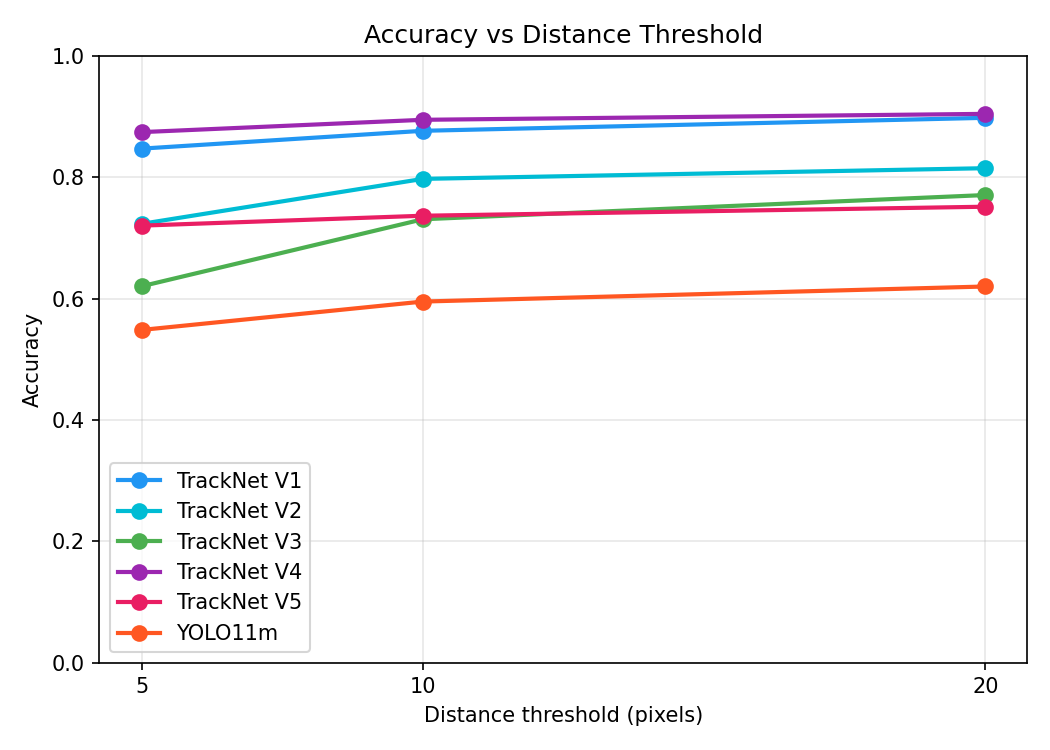
\includegraphics[width=\linewidth]{img/ball_accuracy_curves.png}
    \caption{Accuracy versus distance tolerance.}
    \label{fig:ball-acc-curves}
  \end{subfigure}\hfill
  \begin{subfigure}{0.49\textwidth}
    \centering
    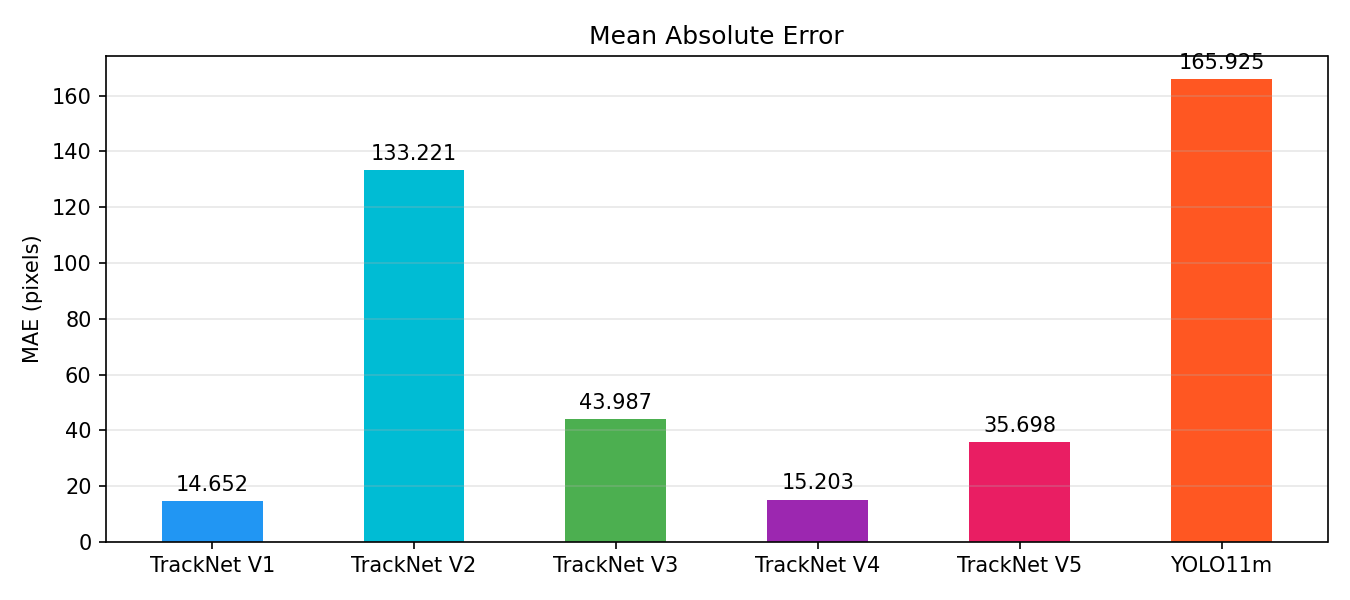
\includegraphics[width=\linewidth]{img/ball_mae_comparison.png}
    \caption{Mean absolute error.}
    \label{fig:ball-mae}
  \end{subfigure}

  \vspace{0.7em}
  \begin{subfigure}{0.49\textwidth}
    \centering
    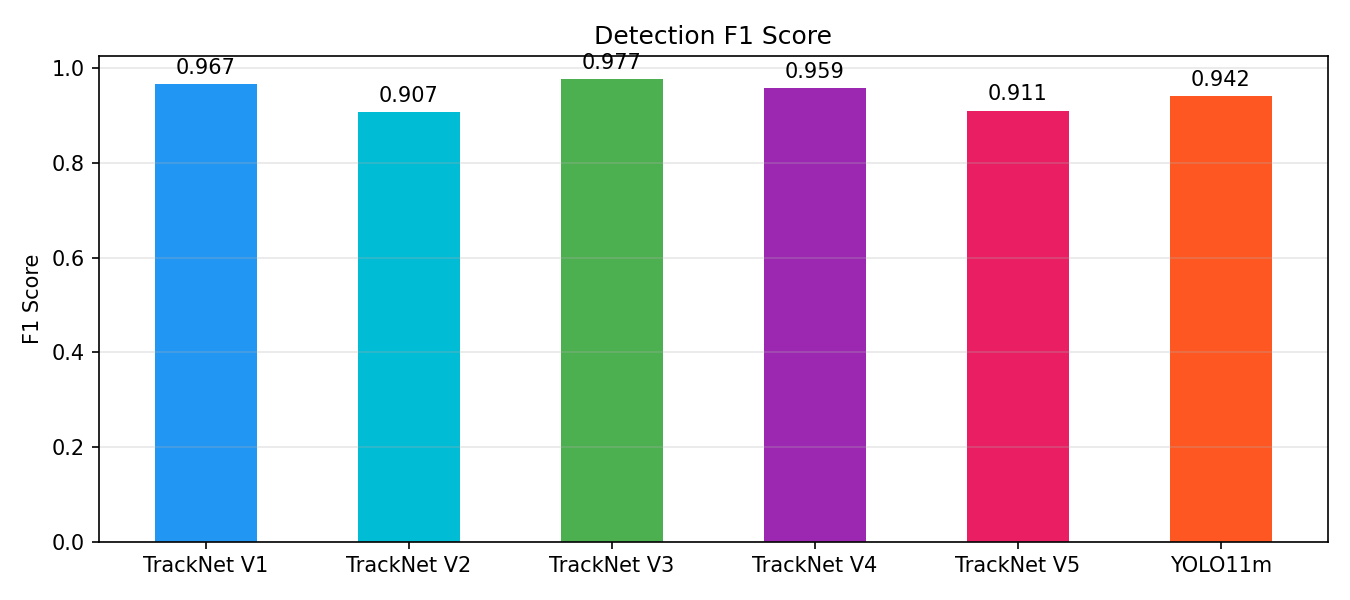
\includegraphics[width=\linewidth]{img/ball_f1_comparison.png}
    \caption{Detection $F_1$.}
    \label{fig:ball-f1}
  \end{subfigure}

  \vspace{0.7em}
  \begin{subfigure}{0.62\textwidth}
    \centering
    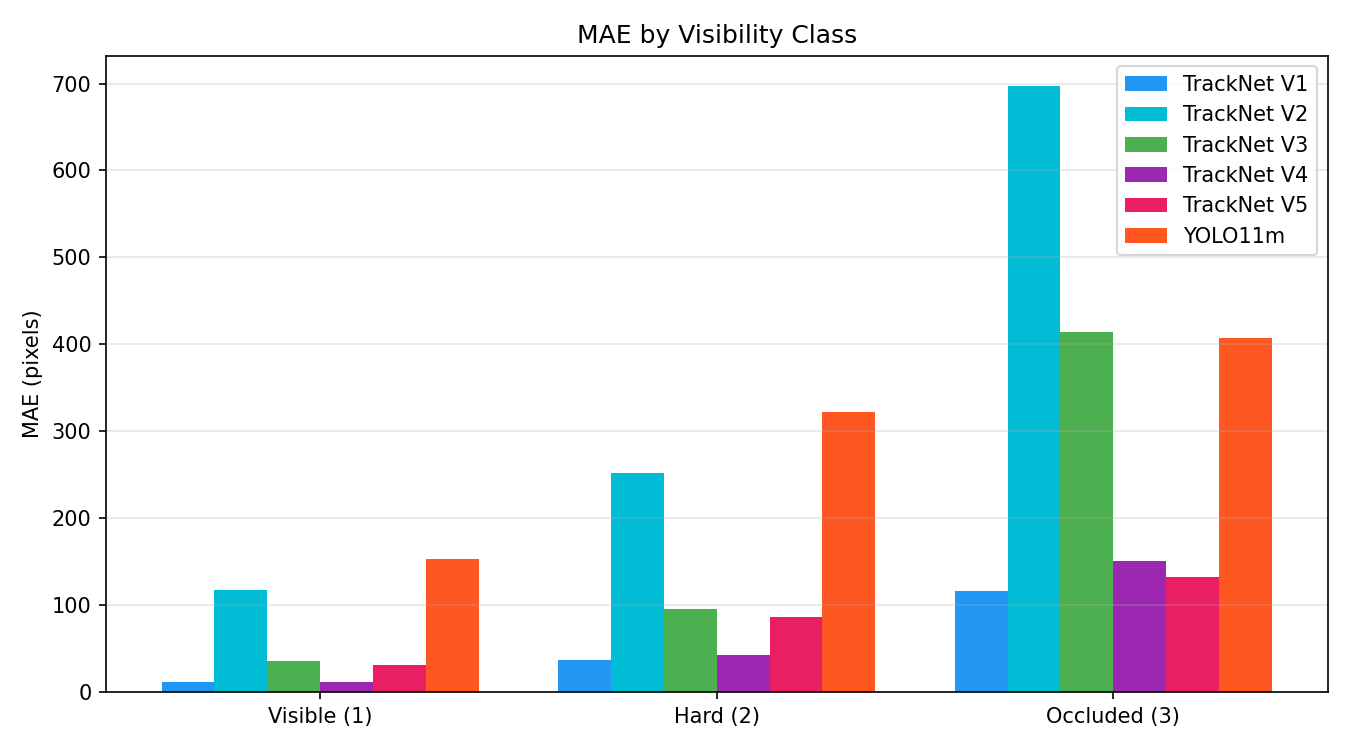
\includegraphics[width=\linewidth]{img/ball_visibility_mae.png}
    \caption{Mean absolute error by visibility class.}
    \label{fig:ball-vismae}
  \end{subfigure}

  \caption{Six-model comparison on the subset test match (game7); the plotted
    values are those tabulated in Table~\ref{tab:ball-selection}.
    (a)~Localisation accuracy across the $\{5, 10, 20\}$-pixel tolerance sweep,
    where TrackNetV4 and V1 lead while YOLO11m trails. (b)~Mean absolute error
    and (c)~detection $F_1$. (d)~Mean
    absolute error split by visibility class, showing that all models degrade
    from clearly visible to occluded balls, with the heaviest tails for V2 and
    YOLO11m.}
  \label{fig:ball-selection}
\end{figure}

\subsection{The case for TrackNetV4}
\label{sec:ball-selection-why}

TrackNetV4 was selected on three grounds. First, it is the strongest localiser
at strict tolerance: it attains the highest accuracy at all three thresholds,
and in particular the highest acc@5px (0.875), the most demanding and the most
decision-relevant of the localisation metrics for a ball whose position must
later feed a geometric line call. Second, it produces the smoothest track, with
the lowest tracking consistency of all six models (10.44 pixels), below V1's
13.98 and far below the V2, V3, and YOLO values; a steady trajectory directly
benefits the downstream bounce detector and the court projection. Third, it is
among the fastest, at 53.07 frames per second, effectively tied with the
quickest model and between two and four times the throughput of V2, V3, and V5.
TrackNetV4 therefore sits at the favourable corner of the accuracy-speed
trade-off, offering the best strict-tolerance accuracy at a negligible cost in
speed.

The remaining models were not selected for reasons that the table makes
concrete. V1 is the only genuine rival: it records a marginally lower mean error
(14.65 against 15.20 pixels), higher recall (0.966 against 0.937), and a few
more frames per second, but its acc@5px is lower and its track is noticeably
jitterier, so V4's motion attention is read as buying sharper and steadier
localisation at the strict tolerance for almost no speed penalty. V2 attains the
highest precision but its recall collapses to 0.831 and its mean error is
catastrophic at 133 pixels, indicating that it frequently fails to localise the
ball at all on this subset. V3 has the best recall and $F_1$, meaning it finds
the ball most often, yet it records the lowest acc@5px of the TrackNet family
(0.620) and the lowest throughput (13.73 frames per second): its inpainting
rectifier recovers the presence of the ball without recovering its precise
position. V5 is middling on every axis, suggesting that learned temporal
self-attention adds parameters and cost without an accuracy gain over the
explicit motion cue of V4 on this data. YOLO11m is the weakest localiser
overall, with the lowest acc@5px (0.548), a mean error of 166 pixels, and by far
the jitteriest track (74.79), which is consistent with the expectation that
box-centre regression localises a tiny ball less precisely than dense heatmap
regression.

These observations answer RQ1 directly. The progression from V1 to V5 is not
monotone in accuracy: the later variants are not uniformly better, and the
strongest strict-tolerance localiser is V4, whose motion-attention mechanism
proves to be the most effective of the temporal modules tried. The single-frame
bounding-box detector is clearly inferior to the heatmap trackers for this
target, which supports the thesis's broader claim that heatmap regression is the
more suitable formulation for a small, fast ball.

\section{Final Model's Results: TrackNetV4 on the Full Dataset}
\label{sec:ball-final}

The second stage retrained the selected model, TrackNetV4, on the full dataset
split of Section~\ref{sec:meth-splits-tracknet}: matches game1 through game9
for training and validation, and game10 held out in its entirety as the test
match. Its closest rival from the selection stage, the original TrackNet (V1),
was retrained on the identical split as a reference baseline, to test whether
the architecture ranking of Section~\ref{sec:ball-selection} survives the move
to the full dataset. Training of TrackNetV4 ran for 100 epochs and recorded a
best validation acc@5px of 0.938 at epoch~73; its loss and validation-accuracy
curves are shown in Figure~\ref{fig:ball-v4-training}. Both models were then
evaluated on the unseen game10 test match, and the resulting test metrics are
reported in Table~\ref{tab:ball-final}. These figures are the headline ball
result of the thesis; they are measured on a different and larger split than the
selection numbers of Table~\ref{tab:ball-selection} and must not be compared
column-for-column with them.

\begin{figure}[t]
  \centering
  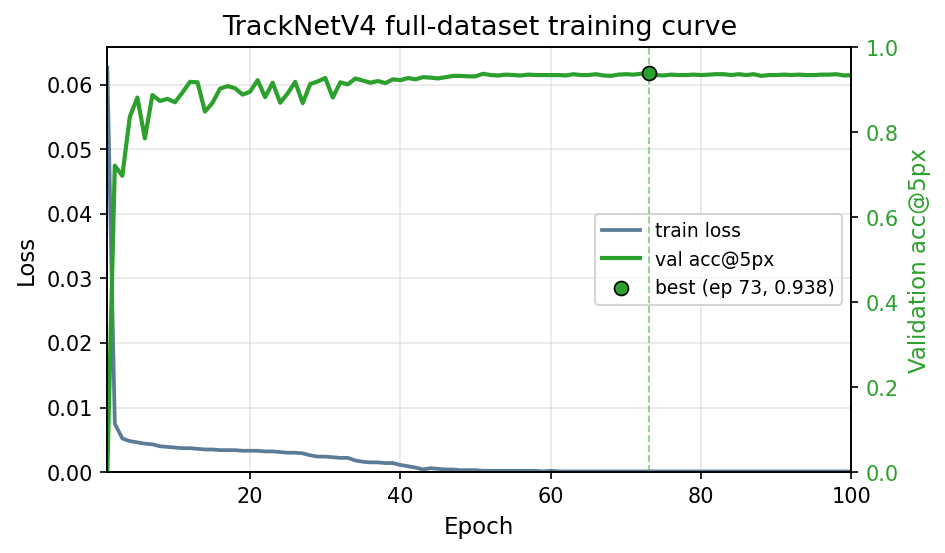
\includegraphics[width=0.8\textwidth]{img/ball_v4_training_curves.png}
  \caption{Training curve of the final TrackNetV4 on the full dataset split
    (game1--game9 for training and validation). The training loss (left axis) and
    validation accuracy at five pixels (right axis) are both plotted on linear
    scales against the epoch count. The training loss falls steeply over the first
    few epochs and then continues to decrease; validation acc@5px climbs to a plateau
    around 0.93 and peaks at 0.938 at epoch~73 (marked), the checkpoint carried
    forward for evaluation.}
  \label{fig:ball-v4-training}
\end{figure}

\begin{table}[t]
  \centering
  \footnotesize
  \setlength{\tabcolsep}{4pt}
  \caption{Final metrics of TrackNetV4 and its closest rival, the original
    TrackNet (V1), both retrained on the full dataset split and evaluated on the
    held-out test match (game10) at the best validation checkpoint. Bold marks
    the better of the two values in each column; lower is better for the MAE
    columns and tracking consistency (TC). The four MAE columns give the mean
    localisation error in pixels: overall (all) and, split by visibility class,
    for clearly visible (vis1), hard-to-identify (vis2), and occluded (vis3)
    balls. P@5px, R@5px, and $F_1$@5px are the location-aware detection metrics
    of Section~\ref{sec:meth-metrics-det}. The frames-per-second figures were
    measured on different hardware and under a different timing protocol than
    Table~\ref{tab:ball-selection} and are not comparable with that table (see
    text).}
  \label{tab:ball-final}
  \resizebox{\textwidth}{!}{%
  \begin{tabular}{l rrr rrrr rrr rrr rr}
    \toprule
    & \multicolumn{3}{c}{Localisation acc} & \multicolumn{4}{c}{MAE (px)}
    & \multicolumn{3}{c}{Detection} & \multicolumn{3}{c}{Detection @5px}
    & \multicolumn{2}{c}{} \\
    \cmidrule(lr){2-4}\cmidrule(lr){5-8}\cmidrule(lr){9-11}\cmidrule(lr){12-14}
    Model & \makecell[r]{acc@\\5px} & \makecell[r]{acc@\\10px} & \makecell[r]{acc@\\20px}
    & all & vis1 & vis2 & vis3 & Prec & Rec & $F_1$
    & \makecell[r]{P@\\5px} & \makecell[r]{R@\\5px} & \makecell[r]{$F_1$@\\5px}
    & \makecell[r]{TC} & FPS \\
    \midrule
    TrackNet (V1)       & 0.948 & 0.952 & 0.954 & 16.08 & 9.81 & 78.28 & 317.72 & \textbf{1.000} & 0.957 & 0.978 & \textbf{0.990} & 0.948 & \textbf{0.969} & \textbf{7.85} & \textbf{43.65} \\
    \textbf{TrackNetV4} & \textbf{0.956} & \textbf{0.959} & \textbf{0.963} & \textbf{12.13} & \textbf{6.89} & \textbf{63.87} & 317.72 & 0.996 & \textbf{0.972} & \textbf{0.984} & 0.980 & \textbf{0.956} & 0.968 & 8.82 & 40.82 \\
    \bottomrule
  \end{tabular}}
\end{table}

Several features of Table~\ref{tab:ball-final} deserve comment, and they are
relevant to how the numbers are quoted elsewhere in the thesis. First, the
selection-stage ranking holds on the full dataset: TrackNetV4 again leads its
closest rival V1 on strict-tolerance accuracy (acc@5px of 0.956 against 0.948)
and on mean error in every visibility class, while V1 retains the marginally
higher precision (1.000 against 0.996), the smoother track (a tracking
consistency of 7.85 against 8.82 pixels), and a few more frames per second
(43.65 against 40.82). This is the same accuracy-against-smoothness trade-off
seen at selection, now confirmed on a larger and previously unseen match, and it
justifies carrying V4 forward as the system's ball tracker. Second, the
strict-tolerance accuracy of V4 rises substantially relative to the selection
stage, from 0.875 on the subset to 0.956 on the full split, and it does so even
though the final model is scored on a finer $640 \times 368$ grid, on which five
pixels is a stricter tolerance than on the selection stage's $256 \times 256$
grid; the larger and more varied training set, together with the higher
resolution, sharpens localisation on clearly visible balls. The two stages' mean
errors are measured on these different grids and so are not directly comparable
in raw pixels, but the final aggregate of 12.13 pixels for V4 is dominated, as at
selection, by a heavy tail of difficult cases: on clearly visible balls
(visibility class~1) the mean error is tight at 6.89 pixels, whereas on the rare
hard-to-identify balls (class~2) it is 63.87 pixels and on the still rarer
occluded balls (class~3) it is 317.72 pixels. For this reason acc@5px, and not
the mean error, is quoted as the headline localisation figure throughout. The
track remains smooth, with a tracking consistency of 8.82 pixels, and precision
is near-perfect at 0.996 on game10, so that almost every reported ball is a true
positive, while the location-aware $F_1$@5px of 0.968 confirms that the great
majority of detections are also well localised.


\section{Analysis}
\label{sec:ball-analysis}

The selection result and the final metrics together support a coherent picture
of why TrackNetV4 succeeds and where it remains limited. Its advantage traces to
the motion-attention module: by gating the decoder with a map of inter-frame
motion, the network concentrates its capacity on the regions where a fast ball
actually appears, which sharpens the response peak and, as the tracking
consistency shows, steadies the trajectory between frames. This is achieved at
essentially no parameter cost over the V1 backbone, which is why V4 dominates V1
on strict-tolerance accuracy and smoothness while matching it on speed. The
comparison with V5 is instructive in the same vein: the explicit, almost
free motion cue of V4 outperformed the heavier learned temporal self-attention
of V5 on this data, indicating that for this target a strong inductive bias
towards motion is more effective than a general attention mechanism left to
learn the same cue.

The per-visibility breakdown locates the residual difficulty precisely. The
model is accurate when the ball is clearly visible, which is the common case,
but its error grows by an order of magnitude on the motion-blurred and occluded
frames of visibility classes~2 and~3. Figure~\ref{fig:ball-final-overlay} shows
the final model's output on four frames sampled across a held-out game10 rally,
where the predicted ball position (red) tracks the ground truth (green) to
within a few pixels throughout. The dominant failure modes are the ones
that the task formulation anticipates: a ball occluded by a player or the net,
which leaves no peak for the heatmap to find; a ball moving fast enough to blur
across many pixels, which broadens and weakens the response; and a ball near or
beyond the frame edge, which has no well-defined centre. These cases are rare in
the dataset and are reflected in the heavy tail of the mean error rather than in
the strict-tolerance accuracy, but they are the natural targets for the future
work discussed in Chapter~\ref{ch:conclusion}, and they are precisely the
situations in which the downstream trajectory rectification and event detection
must be robust.

\begin{figure}[tbp]
  \centering
  \begin{subfigure}{0.49\textwidth}
    \centering
    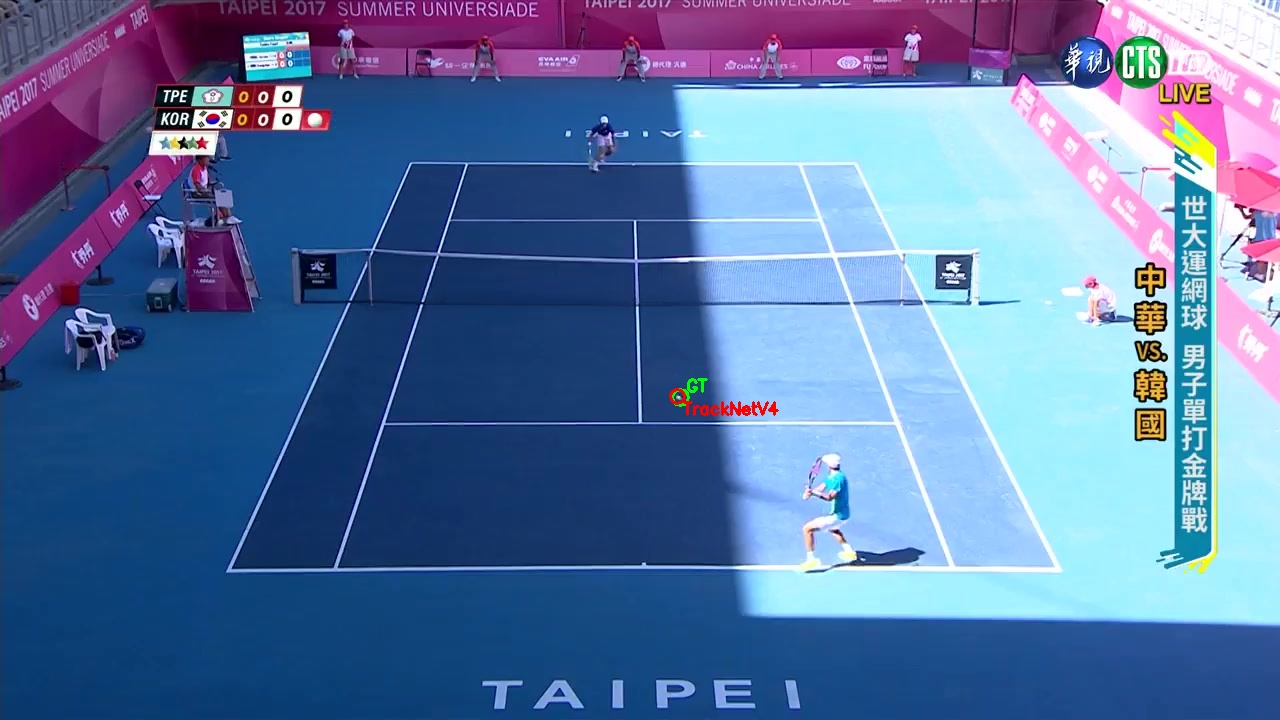
\includegraphics[width=\linewidth]{img/ball_overlay_frame001.jpg}
    \caption{Frame 1.}
    \label{fig:ball-overlay-f1}
  \end{subfigure}\hfill
  \begin{subfigure}{0.49\textwidth}
    \centering
    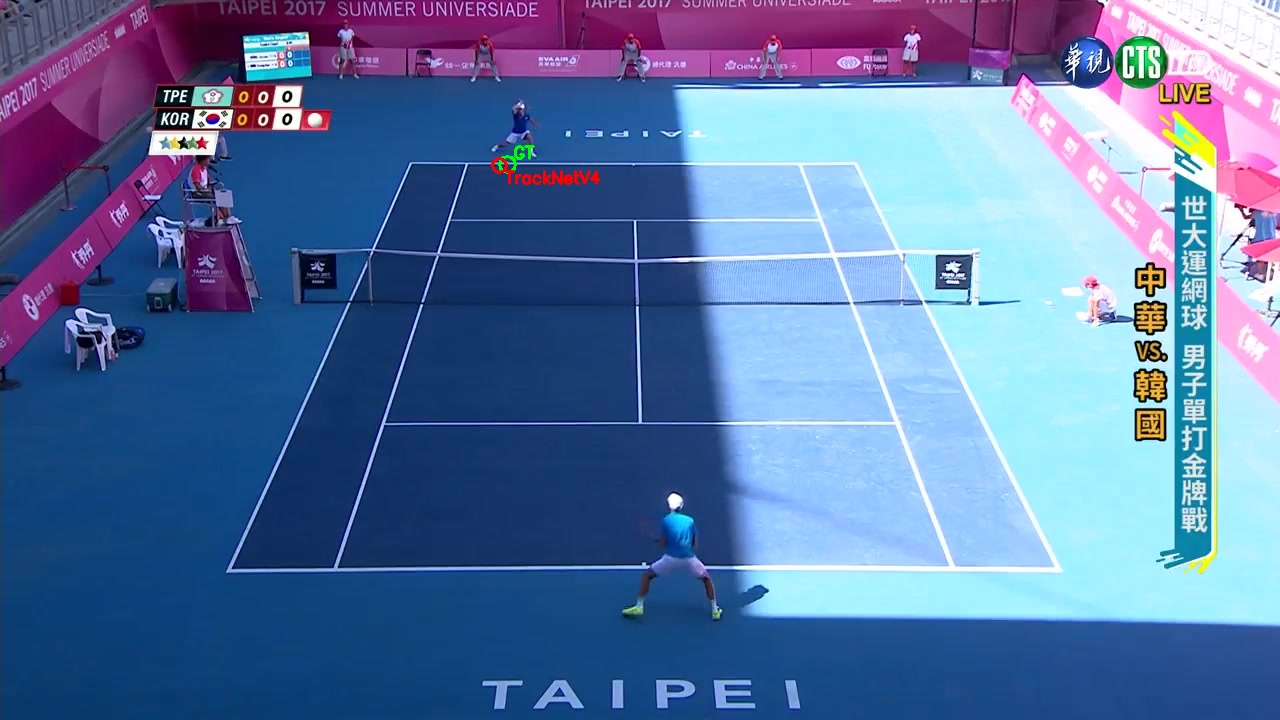
\includegraphics[width=\linewidth]{img/ball_overlay_frame050.jpg}
    \caption{Frame 50 (visibility class~2).}
    \label{fig:ball-overlay-f2}
  \end{subfigure}

  \vspace{0.5em}
  \begin{subfigure}{0.49\textwidth}
    \centering
    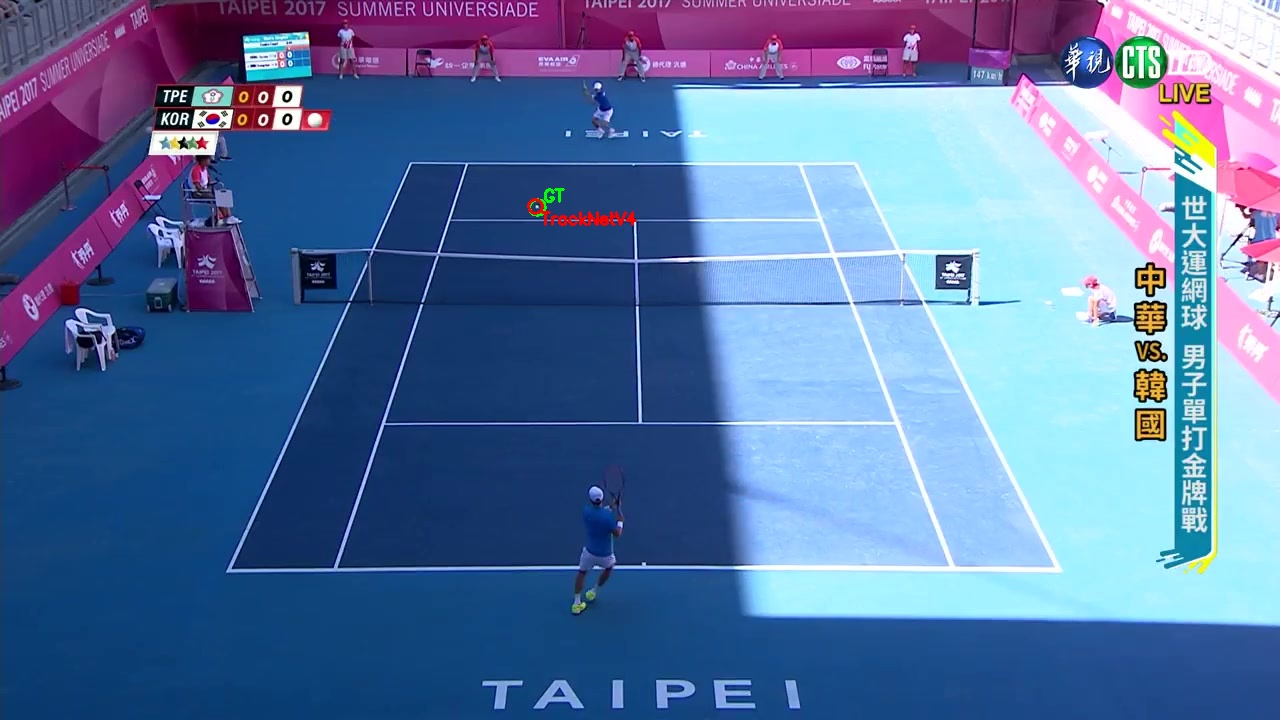
\includegraphics[width=\linewidth]{img/ball_overlay_frame100.jpg}
    \caption{Frame 100.}
    \label{fig:ball-overlay-f3}
  \end{subfigure}\hfill
  \begin{subfigure}{0.49\textwidth}
    \centering
    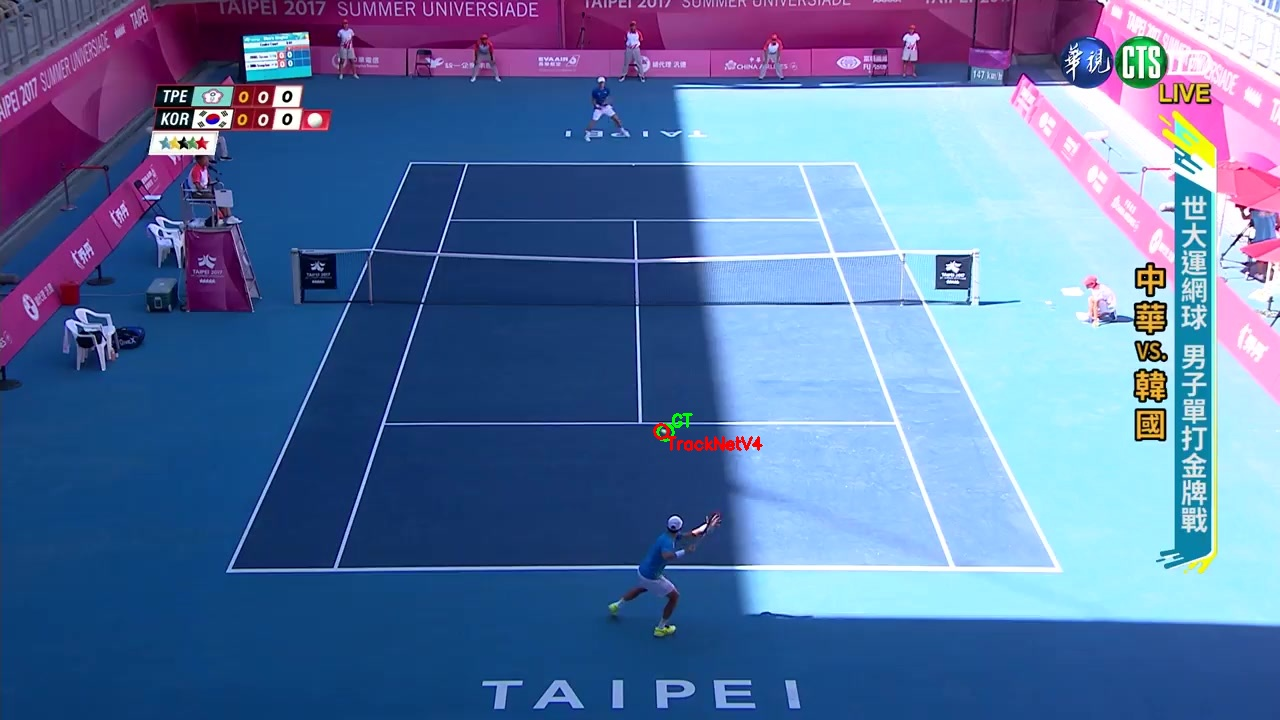
\includegraphics[width=\linewidth]{img/ball_overlay_frame150.jpg}
    \caption{Frame 150.}
    \label{fig:ball-overlay-f4}
  \end{subfigure}
  \caption{Qualitative output of the final TrackNetV4 model on four frames
    sampled across a held-out game10 rally. In each frame the ground-truth ball
    position (green, GT) and the model's prediction (red, TrackNetV4) are
    overlaid; the two markers coincide to within a few pixels throughout,
    including the motion-blurred mid-court frame of visibility class~2~(b). The
    ball is localised accurately across the full range of court positions and
    play phases seen in the rally.}
  \label{fig:ball-final-overlay}
\end{figure}

In summary, the two-stage comparison answers RQ1 by identifying TrackNetV4 as
the best ball-tracking model among the six considered, on the grounds of
strict-tolerance accuracy and trajectory smoothness at competitive speed, and by
showing that the architectural progression through the family is not monotone
and that the heatmap formulation is clearly preferable to single-frame
bounding-box detection for this target. The selected model carries forward to
the integrated system of Chapter~\ref{ch:integrated} as the ball-tracking
component, where its smooth, well-localised trajectory feeds the bounce detector
of Chapter~\ref{ch:bounce} and the court projection of Chapter~\ref{ch:court}.

\chapter{Court Keypoint Detection and Homography}
\label{ch:court}

% Styles for the canonical court schematic (Fig.~\ref{fig:court-template}) and the
% model-head diagrams, kept local to this chapter.
\tikzset{
  courtline/.style={line width=0.9pt, black!75},
  netline/.style={line width=1.3pt, black!85, dash pattern=on 4pt off 2pt},
  kpt/.style={circle, draw=orange!85!black, fill=orange!85!black,
    inner sep=0pt, minimum size=4.2pt},
  kptlbl/.style={font=\scriptsize\bfseries, text=black!80},
  ctr/.style={rectangle, draw=blue!70!black, fill=blue!70!black,
    inner sep=0pt, minimum size=4.2pt},
  dimarr/.style={{Stealth[scale=0.8]}-{Stealth[scale=0.8]}, line width=0.5pt, blue!55!black},
  dimlbl/.style={font=\scriptsize, text=blue!55!black, fill=white, inner sep=1pt},
}

This chapter applies the protocol of Chapter~\ref{ch:methodology} to the second
perception sub-task, locating the fixed landmarks of the tennis court in a single
broadcast frame and using them to register the image to a court-plane coordinate
system. Where ball tracking must follow a small moving target through time, court
detection faces the opposite problem: the landmarks are static and well defined,
but they must be located precisely, because their pixel coordinates feed a
homography whose accuracy in court metres degrades quickly with keypoint error.
Four heatmap models are compared on the court-keypoint dataset of
Section~\ref{sec:meth-court}, a from-scratch baseline and three models built on
pretrained backbones of very different sizes, and each is scored both by the
keypoint-localisation metrics of Section~\ref{sec:meth-metrics-loc} and by the
geometric registration metrics of Section~\ref{sec:meth-metrics-geom}. The
chapter answers the second research question (RQ2) on which backbone gives the
best accuracy against latency trade-off for fourteen-keypoint court detection,
and whether the chosen model is reliable enough to drive a homography into
court-metric space.

Unlike the ball comparison of Chapter~\ref{ch:ball}, the court comparison is a
single-stage one: all four models were trained and evaluated on the one court
split of Section~\ref{sec:meth-splits-court}, with no separate subset-selection
stage, so the numbers in this chapter are directly comparable across models. The
model carried forward into the integrated system of
Chapter~\ref{ch:integrated} is selected here on the combined evidence of accuracy,
geometric registration quality, throughput, and size.

\section{Task and Data Specifics}
\label{sec:court-task}

Court detection is posed as the localisation of fourteen fixed court landmarks in
a single RGB frame, each landmark predicted as the peak of a dedicated heatmap
channel. The fourteen landmarks follow the ordering of the TennisCourtDetector
collection \cite{yastrebksv2023courtdetector} that the dataset is drawn from, and
that ordering is fixed throughout the data pipeline, the models, and the
geometric template, so it is documented once here. Table~\ref{tab:court-keypoints}
lists the fourteen landmarks together with their coordinates in the canonical
court template described in Section~\ref{sec:court-homography}, and
Figure~\ref{fig:court-template} draws them on a scale court diagram. The four
outer corners (indices~0 to~3) are the doubles-court corners; indices~4 to~7 are
the points where the singles sidelines meet the two baselines; indices~8 to~11
are the points where the singles sidelines meet the two service lines; and
indices~12 and~13 are the centre points of the two service lines, where the
centre service line meets them.

\begin{table}[t]
  \centering
  \small
  \setlength{\tabcolsep}{6pt}
  \caption{The fourteen annotated court keypoints in the TennisCourtDetector
    ordering used throughout the court pipeline, with their coordinates in the
    canonical court template of Section~\ref{sec:court-homography}. The template
    origin is the court centre, the $x$ axis runs along the court width towards
    the right sideline, and the $y$ axis runs along the court length towards the
    top baseline; all coordinates are in metres. A fifteenth heatmap channel
    (the court centre) is constructed rather than annotated, as described in the
    text.}
  \label{tab:court-keypoints}
  \begin{tabular}{r l r r}
    \toprule
    Index & Landmark & $x$ (m) & $y$ (m) \\
    \midrule
    0  & top-left outer (doubles) corner       & $-5.485$ & $+11.885$ \\
    1  & top-right outer (doubles) corner      & $+5.485$ & $+11.885$ \\
    2  & bottom-left outer (doubles) corner    & $-5.485$ & $-11.885$ \\
    3  & bottom-right outer (doubles) corner   & $+5.485$ & $-11.885$ \\
    4  & top-left singles baseline corner      & $-4.115$ & $+11.885$ \\
    5  & bottom-left singles baseline corner   & $-4.115$ & $-11.885$ \\
    6  & top-right singles baseline corner     & $+4.115$ & $+11.885$ \\
    7  & bottom-right singles baseline corner  & $+4.115$ & $-11.885$ \\
    8  & top-left service-line point           & $-4.115$ & $+6.400$ \\
    9  & top-right service-line point          & $+4.115$ & $+6.400$ \\
    10 & bottom-left service-line point        & $-4.115$ & $-6.400$ \\
    11 & bottom-right service-line point       & $+4.115$ & $-6.400$ \\
    12 & top centre service point              & $\phantom{+}0.000$ & $+6.400$ \\
    13 & bottom centre service point           & $\phantom{+}0.000$ & $-6.400$ \\
    \bottomrule
  \end{tabular}
\end{table}

\begin{figure}[t]
  \centering
  \begin{tikzpicture}[scale=0.5]
    % court drawn with the length (y, 23.77 m) along the horizontal screen axis
    % and the width (x, 10.97 m) along the vertical screen axis, for compactness.
    % screen = (court_y, court_x).
    % outer doubles rectangle
    \draw[courtline] (-11.885,-5.485) rectangle (11.885,5.485);
    % singles sidelines
    \draw[courtline] (-11.885,-4.115) -- (11.885,-4.115);
    \draw[courtline] (-11.885, 4.115) -- (11.885, 4.115);
    % service lines
    \draw[courtline] (6.40,-4.115) -- (6.40,4.115);
    \draw[courtline] (-6.40,-4.115) -- (-6.40,4.115);
    % centre service line
    \draw[courtline] (-6.40,0) -- (6.40,0);
    % net
    \draw[netline] (0,-5.485) -- (0,5.485);
    \node[dimlbl] at (0,5.95) {net};
    % keypoints (index : screen coords = (court_y, court_x))
    \foreach \i/\y/\x in {%
        0/11.885/-5.485, 1/11.885/5.485, 2/-11.885/-5.485, 3/-11.885/5.485,
        4/11.885/-4.115, 5/-11.885/-4.115, 6/11.885/4.115, 7/-11.885/4.115,
        8/6.40/-4.115, 9/6.40/4.115, 10/-6.40/-4.115, 11/-6.40/4.115,
        12/6.40/0, 13/-6.40/0} {
      \node[kpt] (k\i) at (\y,\x) {};
    }
    % index labels, placed to avoid the lines
    \node[kptlbl, above left=0pt of k0] {0};
    \node[kptlbl, above right=0pt of k1] {1};
    \node[kptlbl, below left=0pt of k2] {2};
    \node[kptlbl, below right=0pt of k3] {3};
    \node[kptlbl, below=1pt of k4] {4};
    \node[kptlbl, above=1pt of k5] {5};
    \node[kptlbl, above=1pt of k6] {6};
    \node[kptlbl, below=1pt of k7] {7};
    \node[kptlbl, above left=-1pt of k8] {8};
    \node[kptlbl, above right=-1pt of k9] {9};
    \node[kptlbl, below left=-1pt of k10] {10};
    \node[kptlbl, below right=-1pt of k11] {11};
    \node[kptlbl, above right=0pt of k12] {12};
    \node[kptlbl, below right=0pt of k13] {13};
    % court centre channel
    \node[ctr] (c) at (0,0) {};
    \node[dimlbl, below right=-1pt of c] {centre};
    % dimensions
    \draw[dimarr] (-11.885,-6.4) -- (11.885,-6.4);
    \node[dimlbl] at (0,-6.4) {$23.77$ m (length)};
    \draw[dimarr] (12.9,-5.485) -- (12.9,5.485);
    \node[dimlbl] at (12.9,0) {$10.97$ m};
    \draw[dimarr] (-12.9,-4.115) -- (-12.9,4.115);
    \node[dimlbl] at (-12.9,0) {$8.23$ m};
    \draw[dimarr] (0,4.7) -- (6.40,4.7);
    \node[dimlbl] at (3.2,4.7) {$6.40$ m};
  \end{tikzpicture}
  \caption{The canonical tennis court template and the fourteen annotated
    keypoints, drawn to scale with the court length along the horizontal axis for
    compactness. Orange discs mark the fourteen annotated landmarks of
    Table~\ref{tab:court-keypoints}, numbered by their channel index; the blue
    square at the centre marks the constructed fifteenth channel. The dashed line
    is the net. Dimensions are the International Tennis Federation court
    specification: a doubles court of $23.77 \times 10.97$ m, a singles width of
    $8.23$ m, and service lines $6.40$ m from the net.}
  \label{fig:court-template}
\end{figure}

The dataset is the publicly distributed TennisCourtDetector collection introduced
in Section~\ref{sec:meth-court}, and Figure~\ref{fig:court-gt} there shows two
annotated frames. Its split is the deterministic, seedless partition of
Section~\ref{sec:meth-splits-court}: the 6\,630 training records are used as
supplied, and the 2\,211 validation records are sorted by identifier and divided
into 1\,105 validation records and the remainder for test. 

\section{Preprocessing and Learning Targets}
\label{sec:court-preproc}

Every frame is resized to a fixed $360 \times 640$ input (height by width), and the predicted keypoints are
scaled back to the original frame resolution for evaluation. The original frames
of this dataset are $1280 \times 720$, so the rescaling factor from the input
back to the original is uniform at a factor of two on each axis; this factor
matters for the strict-tolerance results and is taken up again in
Section~\ref{sec:court-analysis}. Pixel intensities are always divided by 255 to
lie in $[0, 1]$, and for the three models built on ImageNet-pretrained backbones
the per-channel ImageNet mean and standard deviation are additionally subtracted
and divided, so that the inputs match the statistics the backbones were
pretrained on; the from-scratch baseline uses the plain $[0, 1]$ scaling only.

The learning target for each annotated keypoint is a CenterNet-style Gaussian
blob centred on the landmark \cite{zhou2019centernet}, rendered into that
keypoint's heatmap channel at the model's output resolution.

Data augmentation is applied to the training split only. It changes brightness
by up to $\pm 0.3$ of the intensity range, scales contrast by a factor drawn from
$[0.7, 1.3]$, and with probability one half flips the frame horizontally. As in
the ball pipeline, the horizontal flip is the augmentation that interacts with the
labels, and it does so more complicatedly here than for a single ball: flipping the
image left to right not only remaps each keypoint x-coordinate to $W - 1 - x$ but
also rearrange the keypoint indices, because a left landmark becomes a right
landmark. The permutation swaps the symmetric left and right pairs (the two outer
corners, the two singles baseline corners, the singles points, and the service
points) while leaving the two centre service points unchanged, and it is applied
as a fixed index map so that each channel continues to predict the correct
landmark after the flip.

\section{Models}
\label{sec:court-models}

Four models are compared, chosen to span the design space from a faithful
reimplementation of the dataset's own baseline to backbones of widely differing
capacity and cost. All four take a single RGB frame and emit a fifteen-channel
heatmap, and all four are trained under the identical regime described below, so
that the comparison isolates the effect of the backbone and the output
resolution. Table~\ref{tab:court-models} summarises them along the axes that
shape the results.

\begin{table}[t]
  \centering
  \small
  \setlength{\tabcolsep}{5pt}
  \caption{The four court-keypoint models. All emit a fifteen-channel heatmap
    (fourteen landmarks plus the constructed centre). Output stride is the ratio
    of the input resolution to the heatmap resolution: the two stride-1 models
    predict at the full $360 \times 640$ input grid, the two stride-4 models at a
    $90 \times 160$ grid. Parameter counts are computed from the implementations
    used here.}
  \label{tab:court-models}
  \begin{tabular}{@{}l p{3.5cm} p{3.2cm} c c c r@{}}
    \toprule
    Model & Backbone & Decoder / head & \makecell{Out.\\stride} & \makecell{Gauss.\\radius}
          & \makecell{ImageNet\\norm.} & \makecell[r]{Params\\(M)} \\
    \midrule
    TrackNet-court & VGG-style encoder-decoder(from scratch) & transposed-conv decoder with skips & 1 & 15 & no  & 20.8 \\
    ResNet50       & ResNet-50(ImageNet)                      & three transposed-conv blocks       & 4 & 8  & yes & 34.0 \\
    HRNet          & HRNet-W32(timm features)                 & stride-4 feature tap + $1\times1$  & 4 & 8  & yes & 30.9 \\
    MobileNetV3    & MobileNetV3-Small(ImageNet)              & U-Net decoder                       & 1 & 15 & yes & 1.28 \\
    \bottomrule
  \end{tabular}
\end{table}

TrackNet-court is a faithful reimplementation of the baseline shipped with the
dataset \cite{yastrebksv2023courtdetector}, the same VGG-style encoder-decoder
backbone used for ball tracking in Chapter~\ref{ch:ball}
\cite{huang2019tracknet}, adapted to take a single three-channel frame rather
than a stacked window and to emit fifteen channels rather than one. Its decoder
upsamples back to the full input resolution through transposed convolutions with
skip connections, so it predicts at output stride one, a $360 \times 640$ heatmap
per channel, and it is the only model trained from scratch without ImageNet
normalisation.

ResNet50 pairs an ImageNet-pretrained ResNet-50 backbone \cite{he2016resnet} with
the simple-baseline pose decoder of Xiao et al.~\cite{xiao2018simplebaselines}:
three transposed-convolution blocks that upsample the stride-32 backbone features
to a stride-4 heatmap, followed by a $1 \times 1$ convolution to fifteen channels.
It predicts at output stride four, a $90 \times 160$ heatmap, and it is the
heaviest model at thirty-four million parameters.

HRNet is built on an HRNet-W32 backbone. It should be noted that the implementation taps a
stride-4 feature map from the backbone's feature pyramid and applies a
$1 \times 1$ convolutional head, rather than using HRNet's native
full-resolution branch; it is therefore a stride-4 model in the same sense as
ResNet50, and this design choice bears directly on its strict-tolerance accuracy,
as Section~\ref{sec:court-analysis} discusses. It carries thirty-one million
parameters.

MobileNetV3 pairs an ImageNet-pretrained MobileNetV3-Small backbone
\cite{howard2019mobilenetv3}, the efficient inverted-residual architecture in the
MobileNet line \cite{sandler2018mobilenetv2}, with a U-Net-style decoder that
upsamples all the way back to the full input resolution. It therefore predicts at
output stride one, a $360 \times 640$ heatmap, like TrackNet-court, but at a
fraction of the size: at 1.28 million parameters it is roughly one sixteenth the
size of TrackNet-court and one twenty-fifth the size of ResNet50.

All four models output raw logits, with the sigmoid applied inside the loss and
at evaluation. They were trained with a common recipe, the Adam optimiser
\cite{kingma2015adam} with a CenterNet-style penalty-reduced focal loss on the
sigmoid of the predicted heatmaps \cite{zhou2019centernet}, which drives the
response towards one at each keypoint peak while reducing the penalty on the
pixels around it in proportion to their Gaussian target value, a learning rate of
$10^{-4}$ halved on plateau, a batch size of eight, and early stopping with a
patience of thirty epochs. The checkpoint kept for each model is the one with the best validation
accuracy at the seven-pixel tolerance, measured in the resized input space; the
distinction between that monitoring metric and the test metric reported below is
discussed in Section~\ref{sec:court-analysis}. A keypoint coordinate is decoded
from a predicted heatmap by locating the peak channel response, refining it to
sub-pixel precision with a local three-by-three intensity-weighted mean, and
scaling by the output stride and the input-to-original factor; a peak below a
confidence threshold of 0.3 return the no-keypoint.

\section{Homography Estimation}
\label{sec:court-homography}

The motivation for detecting court keypoints precisely is that they anchor a
planar homography, the map from image pixels $(u, v)$ to court-plane coordinates
$(X, Y)$ in metres that turns a detected ball position into a measurement on the
court and so makes a in-or-out decision possible. The court is planar
and the camera projection is perspective, so the image-to-court map is a single
$3 \times 3$ homography. The canonical court template against which the homography
is fitted is the metric layout of Table~\ref{tab:court-keypoints} and
Figure~\ref{fig:court-template}: a doubles court of $23.77 \times 10.97$ m with
the origin at the court centre, built directly from the International Tennis
Federation court dimensions, the singles width of $8.23$ m and the service lines
$6.40$ m from the net.

The homography is estimated from the detected keypoints with a
random-sample-consensus fit, known as RANSAC \cite{fischler1981ransac}, which is essential here
because individual keypoints can be missed or mislocated and a least-squares fit
to all of them would be corrupted by a single gross outlier. The procedure
filters out any keypoint carrying the missing detections, then fits a homography
from the canonical template points to their detected image positions with a RANSAC
reprojection threshold of five pixels, which keeps the threshold in the intuitive
image-pixel units. At least four visible keypoints are required for a homography
to be defined, and the fit is accepted only if at least six of the points are
RANSAC inliers, so that an estimate is reported only when it is well supported;
the accepted image-to-court map is then the inverse of the fitted template-to-image
transform.

Two evaluation quantities follow from this estimate, as defined in
Section~\ref{sec:meth-metrics-geom}. The homography success rate is the fraction
of test frames for which an accepted homography could be estimated at all, and it
measures how often the detector produces a usable geometric registration. The
mean reprojection error in centimetres measures the geometric quality of an
accepted homography: the visible ground-truth keypoints are projected through the
predicted homography into the court plane and their displacement from the
canonical template positions is measured in court metres, then expressed in
centimetres.

\section{Results}
\label{sec:court-results}

The four models were evaluated on the 1100 record court test set, with all
keypoint coordinates scaled back to the original $1280 \times 720$ resolution
before scoring. Table~\ref{tab:court-results} reports the keypoint-localisation
metrics, the geometric registration metrics, and the size and throughput of each
model; Figure~\ref{fig:court-comparison} plots the accuracy, error, and size
relationships, and Figure~\ref{fig:court-perkp} breaks the seven-pixel accuracy
down by keypoint.

\begin{table}[t]
  \centering
  \footnotesize
  \setlength{\tabcolsep}{3pt}
  \caption{Court-keypoint results on the held-out test set, with predictions in
    original $1280 \times 720$ pixel space. PCK@$\tau$px is the percentage of
    correct keypoints within $\tau$ pixels; $\mathrm{MAE_{px}}$ is the mean
    keypoint error; reproj.\ is the mean court-plane reprojection error in
    centimetres; succ.\ is the homography success rate. Bold marks the best value
    in each column; lower is better for $\mathrm{MAE_{px}}$ and the reprojection
    error. The frames-per-second figures were all measured in a single comparison
    run on one machine and are internally comparable as a ranking, but they
    include the per-frame keypoint decoding and homography estimation and are not
    a pure inference-throughput claim.}
  \label{tab:court-results}
  \begin{tabular}{l rrrr r r r r}
    \toprule
    & \multicolumn{4}{c}{PCK (localisation)} & & \multicolumn{1}{c}{Homog.} &  & \\
    \cmidrule(lr){2-5} \cmidrule(lr){7-7}
    Model & \makecell[r]{@5px} & \makecell[r]{@7px} & \makecell[r]{@10px} & \makecell[r]{@25px}
          & \makecell[r]{$\mathrm{MAE_{px}}$} & \makecell[r]{reproj.\\(cm)}
          & \makecell[r]{Params\\(M)} & FPS \\
    \midrule
    TrackNet-court & 0.970 & 0.988 & 0.995 & 0.998 & 3.46 & \textbf{7.47}  & 20.8 & 4.45 \\
    ResNet50       & 0.388 & 0.688 & 0.960 & 0.996 & 8.24 & 30.58  & 34.0 & 8.67 \\
    HRNet          & 0.460 & 0.849 & 0.986 & 0.998 & 5.98 & 30.78  & 30.9 & 10.42 \\
    \textbf{MobileNetV3} & \textbf{0.974} & \textbf{0.992} & \textbf{0.997} & \textbf{0.999}
                   & \textbf{2.46} & 7.67 & \textbf{1.28} & \textbf{21.00} \\
    \bottomrule
  \end{tabular}
\end{table}

\begin{figure}[p]
  \centering
  \begin{subfigure}{0.49\textwidth}
    \centering
    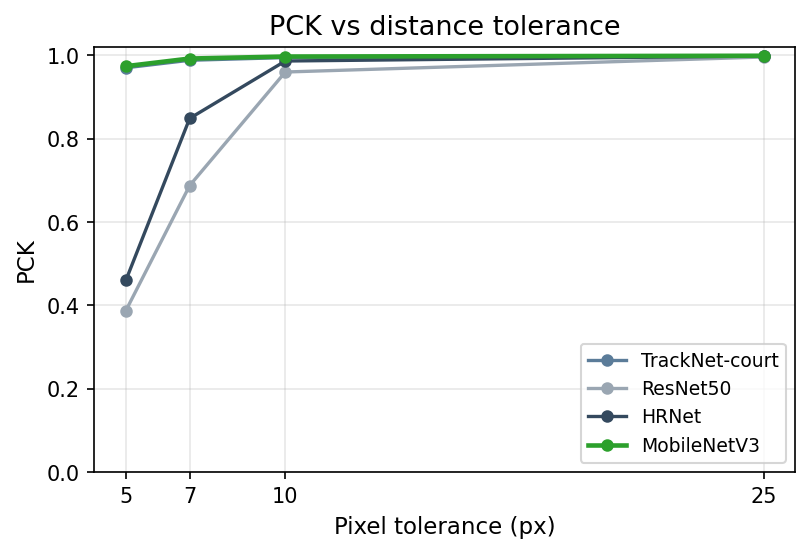
\includegraphics[width=\linewidth]{img/court_pck_curves.png}
    \caption{PCK across the tolerance sweep.}
    \label{fig:court-pck-curves}
  \end{subfigure}\hfill
  \begin{subfigure}{0.49\textwidth}
    \centering
    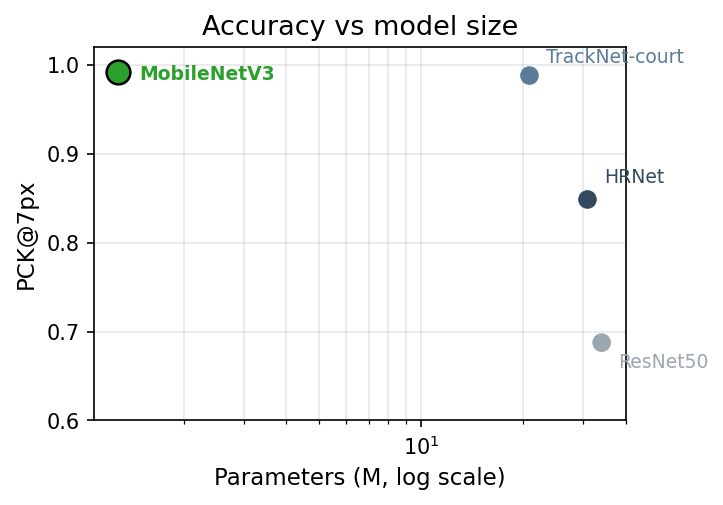
\includegraphics[width=\linewidth]{img/court_params_vs_pck.png}
    \caption{Accuracy against model size.}
    \label{fig:court-params}
  \end{subfigure}

  \vspace{0.7em}
  \begin{subfigure}{0.49\textwidth}
    \centering
    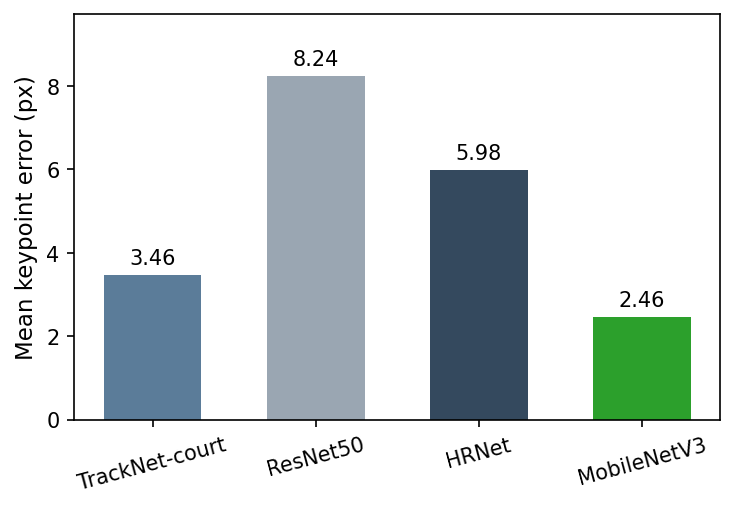
\includegraphics[width=\linewidth]{img/court_mean_kp_error.png}
    \caption{Mean keypoint error.}
    \label{fig:court-mae}
  \end{subfigure}\hfill
  \begin{subfigure}{0.49\textwidth}
    \centering
    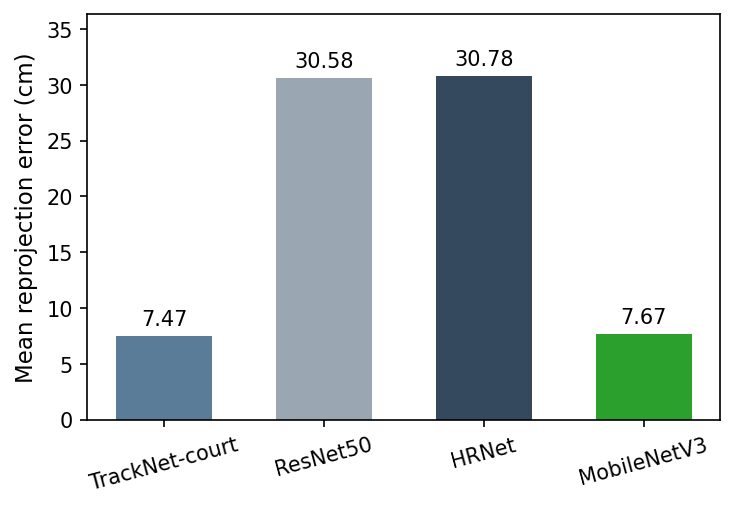
\includegraphics[width=\linewidth]{img/court_reproj_error.png}
    \caption{Mean court-plane reprojection error.}
    \label{fig:court-reproj}
  \end{subfigure}

  \caption{Four-model court-keypoint comparison; the plotted values are those of
    Table~\ref{tab:court-results}. (a)~The percentage of correct keypoints across
    the $\{5, 7, 10, 25\}$-pixel tolerance sweep, where the two output-stride-one
    models (TrackNet-court and MobileNetV3) lead at every tolerance while the two
    stride-four models (ResNet50 and HRNet) start far lower at five pixels and
    converge towards the others only as the tolerance widens. (b)~Accuracy at
    seven pixels against parameter count on a logarithmic axis, showing
    MobileNetV3 at the favourable corner, the smallest model at the top accuracy.
    (c)~Mean keypoint error and (d)~mean court-plane reprojection error per
    model, on both of which MobileNetV3 and TrackNet-court are far ahead of the
    two stride-four models.}
  \label{fig:court-comparison}
\end{figure}

The headline result is that MobileNetV3, by far the smallest of the four models,
is also the most accurate on every metric but one. It attains the best accuracy
at all four tolerances, including the most demanding five-pixel and seven-pixel
thresholds (0.974 and 0.992), the lowest mean keypoint error (2.46 pixels), the
joint-best homography success rate (0.999), and the highest throughput in the
comparison, while carrying 1.28 million parameters against the twenty to
thirty-four million of the others. Its median keypoint error is 1.45 pixels,
which shows that the bulk of its detections are localised to within a pixel or
two and that the mean is inflated by a small tail of harder frames; the same
holds for TrackNet-court, whose median error is 1.44 pixels. The single metric on
which MobileNetV3 does not lead is the mean reprojection error, where
TrackNet-court is marginally better at 7.47 centimetres against 7.67, a
difference too small to separate the two models in practice and far smaller than
the gap to the remaining two.

TrackNet-court, the dataset's own baseline architecture, is the second strongest
model and confirms that the task is well within reach of a heatmap detector: it
reaches 0.988 accuracy at seven pixels and the best reprojection error, but it
does so with sixteen times the parameters of MobileNetV3 and at the lowest
throughput of the four. ResNet50 and HRNet, despite being the two largest and
most capable backbones, are the two weakest court detectors at strict tolerance.
ResNet50 reaches only 0.388 accuracy at five pixels and 0.688 at seven, and HRNet
0.460 and 0.849, both far below the stride-one models, and their mean
reprojection errors of around thirty centimetres are four times worse. Their
accuracy recovers sharply as the tolerance widens, to 0.960 and 0.986 at ten
pixels and to near-parity with the others at twenty-five pixels, which indicates
that they place each keypoint in the right neighbourhood but not to the pixel
precision the strict thresholds demand. The reason for this pattern, which turns
on the output resolution of the models rather than on the capacity of their
backbones, is the subject of Section~\ref{sec:court-analysis}.

\begin{figure}[t]
  \centering
  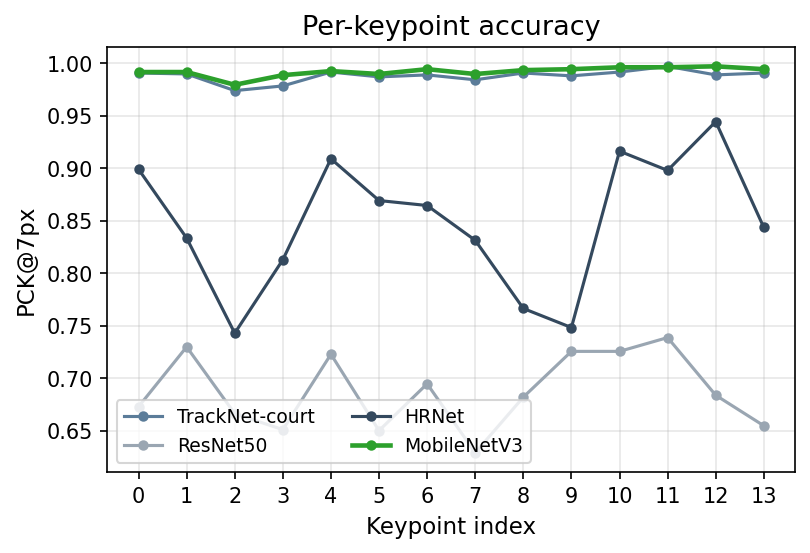
\includegraphics[width=0.85\textwidth]{img/court_per_keypoint_pck.png}
  \caption{Accuracy at seven pixels for each of the fourteen keypoints. The two
    stride-one models are uniformly high across all landmarks, whereas the two
    stride-four models are lower across every landmark rather than failing on any
    particular one, which is consistent with a resolution-limited rather than a
    landmark-specific cause.}
  \label{fig:court-perkp}
\end{figure}

The per-keypoint breakdown of Figure~\ref{fig:court-perkp} shows that no single
landmark dominates the error: the two strong models are uniformly accurate across
all fourteen keypoints, and the two weaker models are uniformly less accurate
rather than failing on a particular corner, which is consistent with a
resolution-limited rather than a landmark-specific cause. The homography success
rate is at least 0.995 for every model, so all four almost always produce enough
well-supported keypoints to register the court; the models are separated by the
precision of that registration, not by whether it can be obtained.
Figure~\ref{fig:court-qualitative} shows a qualitative example of the selected
model's output on a test frame, with the predicted keypoints close to the
ground-truth annotations across the visible court.

\begin{figure}[t]
  \centering
  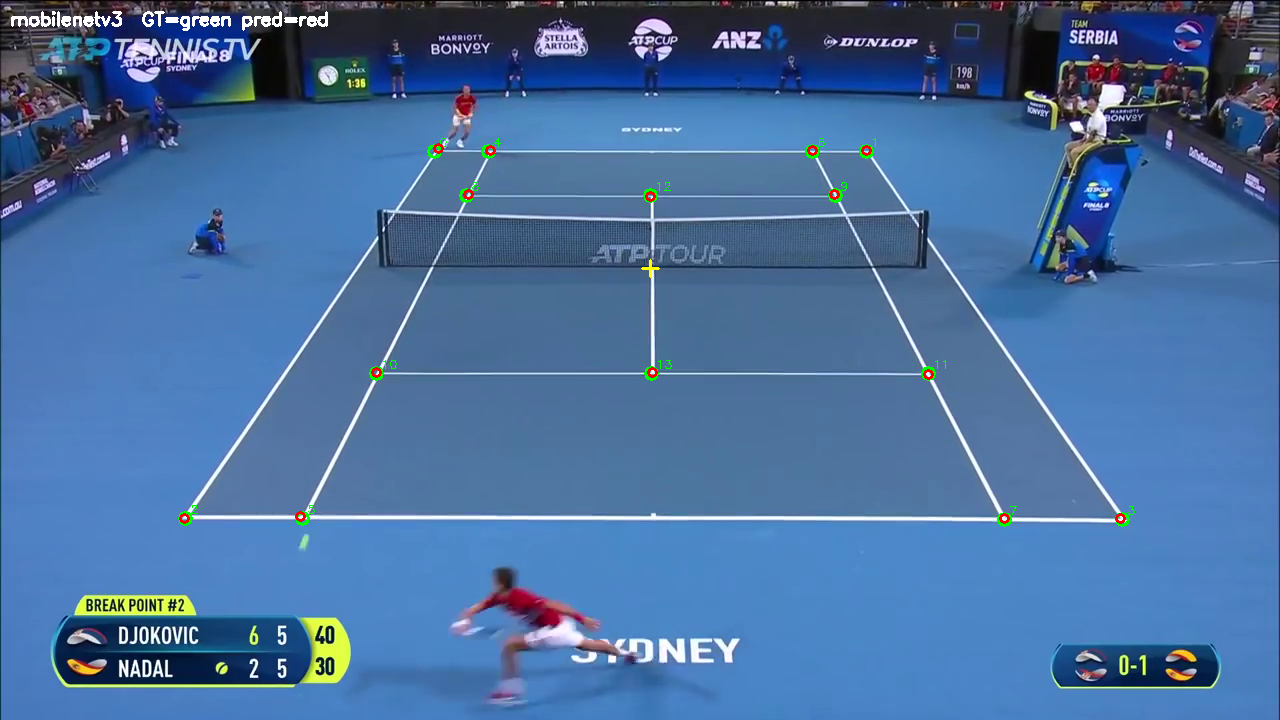
\includegraphics[width=0.8\textwidth]{img/court_overlay_mobilenetv3.png}
  \caption{Qualitative output of the selected MobileNetV3 model on a court test
    frame. Ground-truth keypoints are shown in green, the model's predictions in
    red, and the predicted court centre as a yellow cross. The predicted
    landmarks coincide closely with the ground truth across the court, including
    the far baseline where perspective foreshortening is strongest.}
  \label{fig:court-qualitative}
\end{figure}

These results answer RQ2. Among a heatmap baseline and three backbones of widely
differing size, the best accuracy against latency trade-off is given not by the
largest backbone but by the smallest, a 1.28-million-parameter MobileNetV3-Small
with a full-resolution decoder, which is the most accurate model at every
tolerance and the fastest in the comparison. Its mean court-plane reprojection
error of 7.67 centimetres, obtained on essentially every test frame, is small
relative to the scale of the court and the margins involved in a line call, so it
is reliable enough to drive the homography that the integrated system of
Chapter~\ref{ch:integrated} depends on, and it is the model selected for that
system.

\section{Analysis}
\label{sec:court-analysis}

The central finding of this chapter is that strict-tolerance accuracy on this
task is governed by the output resolution of the heatmap rather than by the
capacity of the backbone, and the four models divide cleanly along that line. The
two models that predict at output stride one, TrackNet-court and MobileNetV3,
emit a heatmap at the full $360 \times 640$ input grid, so that a single heatmap
cell corresponds to one input pixel and, after the factor-of-two rescaling to the
original frame, to about two pixels in the space where accuracy is measured. The
two models that predict at output stride four, ResNet50 and HRNet, emit a
$90 \times 160$ heatmap, so that one cell corresponds to four input pixels and to
about eight pixels in the original frame. The peak of a coarse heatmap can
therefore be no more precise than its cell, and although the sub-pixel refinement
of Section~\ref{sec:court-models} interpolates within a cell it cannot escape the
underlying lattice. A five-pixel tolerance is smaller than the eight-pixel
quantisation of the stride-four models, so even a perfectly centred prediction
frequently falls outside it, which is why ResNet50 and HRNet score so low at five
and seven pixels; once the tolerance widens past the quantisation step, at ten and
twenty-five pixels, a correctly identified cell almost always falls within
tolerance and the two models recover. The stride-one models, with a two-pixel
quantisation, sit comfortably inside even the five-pixel tolerance, which is why
they saturate the accuracy metric. The mean keypoint errors tell the same story
in pixel terms, around six and eight pixels for the stride-four models against
two and three for the stride-one models.

This explanation also resolves an apparent contradiction with the validation
figures used during training. The metric monitored for early stopping and
checkpoint selection was the accuracy at seven pixels measured in the resized
$360 \times 640$ input space, and on that metric all four models reach
comparable, high values, between 0.99 and 0.997. The seven-pixel tolerance in the
input space corresponds to a fourteen-pixel tolerance in the original frame, which
is wide enough to hide the quantisation penalty of the stride-four models;
measuring the test accuracy in the original space at seven pixels, the stricter
and more honest setting, is what exposes it. The lesson is methodological: the
space in which a pixel tolerance is applied must be stated alongside the number,
because the same nominal tolerance describes a different physical accuracy in the
input space and in the original space, and the input-space monitoring metric
flattered the coarse models.

It follows that the comparison is not a refutation of the larger backbones as
feature extractors but of the particular stride-four heads used here, and in the
case of HRNet of a head that does not exploit the backbone's defining
high-resolution branch. A fairer test of ResNet50 and HRNet would attach a decoder
that restores the full resolution, as the U-Net decoder does for MobileNetV3, and
their accuracy would be expected to rise accordingly. The practical conclusion for
this thesis is nonetheless robust: a lightweight, full-resolution model already
saturates the accuracy this task requires while costing a fraction of the
parameters and running fastest, so there is no accuracy argument for paying the
size and latency of the heavier models, and the small-backbone choice is the right
one for a deployable system.

Two further points qualify the results. First, the mean reprojection error in
centimetres should be read as an indicative geometric figure rather than an exact
one, because of how it is computed: ground-truth keypoints are projected through
the homography that was fitted to the predicted keypoints, so the number combines
the accuracy of the keypoints with the quality of the homography fit in a single
quantity, and a maximum reprojection error of well over a metre on the worst
frames, even for the strong models, reflects the occasional frame on which a
degenerate or poorly conditioned fit projects points far from their true
positions. The success rate and the mean error together, rather than either
alone, characterise the registration. Second, the court-centre channel that every
model emits is supervised during training but is not scored at evaluation, because
no ground-truth target for it is constructed in the evaluation loop; its accuracy
is therefore reported as not evaluated, and the channel serves only as an
auxiliary training signal and as an input to the geometric centre used elsewhere.

A local Hough-line refinement of the detected keypoints, which snaps each
prediction towards the nearest painted court line, was also explored as an
optional post-processing step. On the selected model it reduced the accuracy and
the throughput while changing the reprojection error only marginally, so it offers
no clear benefit at the operating point reached here and was not adopted for the
integrated system. Finally, the six excluded test records noted in
Section~\ref{sec:court-task} are a reminder that public datasets carry annotation
noise: they were found by a manual audit of the ground truth, and excluding them
prevents a handful of geometrically impossible annotations from distorting the
test metrics. Their identifiers are recorded in the project so that the exclusion
is reproducible.

In summary, the court comparison answers RQ2 by selecting a 1.28-million-parameter
MobileNetV3-Small model that is the most accurate of the four at every tolerance,
registers the court to within about eight centimetres on essentially every frame,
and runs fastest, and by showing that the accuracy ceiling on this task is set by
the heatmap output resolution rather than by backbone capacity. The selected model
provides the court geometry for the integrated system of
Chapter~\ref{ch:integrated}, where its homography projects the tracked ball and
the detected bounce into the court plane for the in-or-out line call.

\chapter{Bounce Event Detection}
\label{ch:bounce}

This chapter applies the protocol of Chapter~\ref{ch:methodology} to the third
perception sub-task: deciding at which frames the ball bounces on the court, given
the trajectory it traces through a rally. Ball tracking locates the ball in each
frame (Chapter~\ref{ch:ball}) and court detection registers the playing surface
(Chapter~\ref{ch:court}); bounce detection differs from both in that it consumes
the output of the tracker rather than the raw image. Its input is a
one-dimensional time series of ball positions, and its task is to mark the moment
of ground contact within it. The sub-task runs on the TrackNet tennis dataset of
Section~\ref{sec:meth-tracknet}, under the bounce-specific split of
Section~\ref{sec:meth-splits-tracknet} that holds out match game7 as the test set,
and it is scored by the event-detection metrics of
Section~\ref{sec:meth-metrics-event}. Two learned models are trained for that: a
gradient-boosted per-frame classifier and a small temporal convolutional network,
compared on one shared trajectory pipeline. The chapter answers the third
research question (RQ3) of Section~\ref{sec:intro-objectives}: how the two models
compare in accuracy, and what each costs in engineering effort.

\section{Task Formulation}
\label{sec:bounce-task}

A bounce is the frame at which the ball hits the court, recorded in the dataset
as status~2 in the annotation schema of Section~\ref{sec:meth-tracknet-schema}.
The task is posed as event detection in time rather than as per-frame
classification, for the reason set out in Section~\ref{sec:meth-metrics-event}:
bounce frames make up only 2.6\,\% of the data
(Table~\ref{tab:tracknet-labels}), so a per-frame accuracy would be dominated by
the negative class.

The problem is that the signature of a bounce is not unique to bounces. That is what
makes the task hard and rules out a simple solution. A racket hit, status~1 in the
same schema and almost as frequent as a bounce (516 against 523 events across the
dataset, Table~\ref{tab:tracknet-labels}).
Figure~\ref{fig:bounce-trajectory-motivation} shows both effects within a single
rally. Separating a bounce from a hit depends on the finer shape of the
trajectory around the reversal, which neither the reversal nor the ball's position
reveals on its own. That shape is the distinction the two learned models are
trained to understand.

\begin{figure}[t]
  \centering
  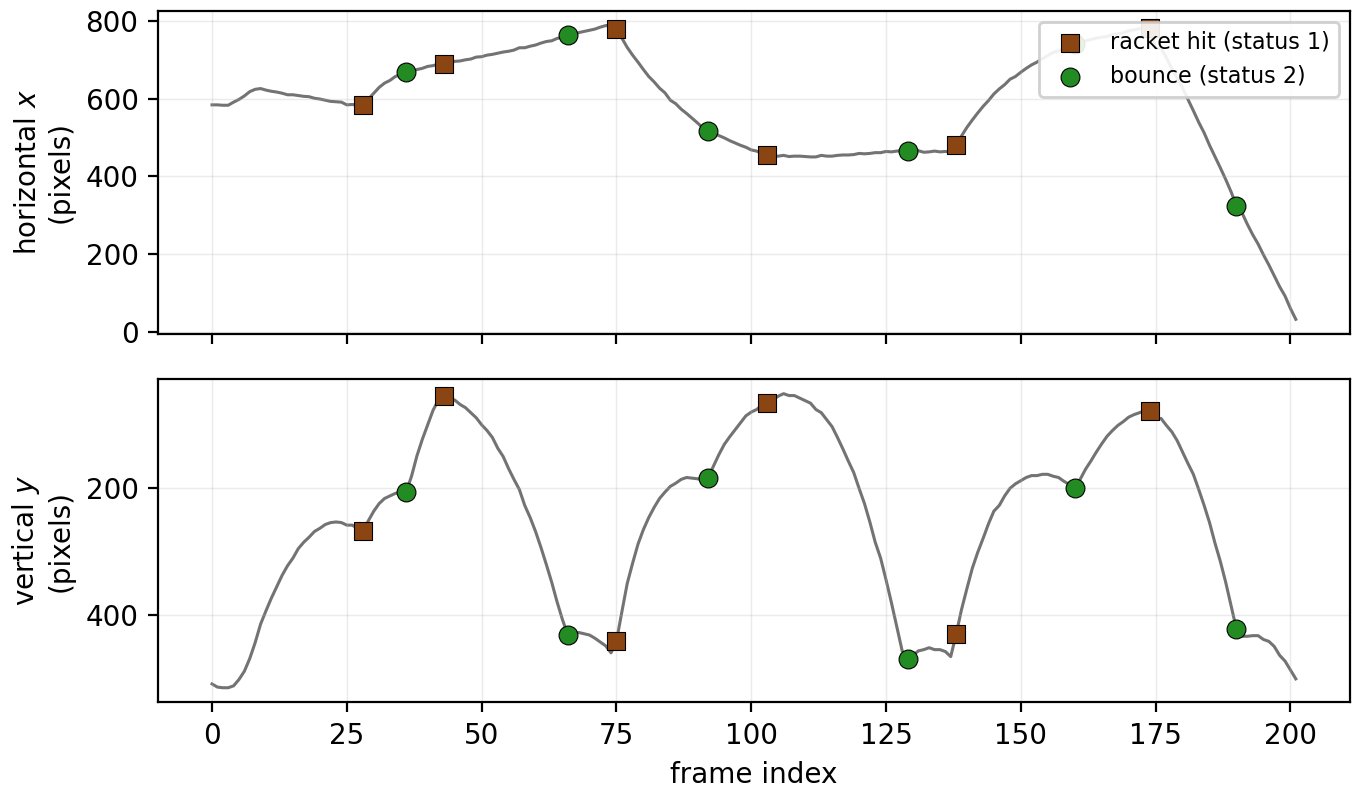
\includegraphics[width=\linewidth]{img/bounce_trajectory_motivation.png}
  \caption{The bounce signature in the ball-coordinate time series, for one rally
    of the game7 test split with six bounces and six hits. The horizontal ($x$)
    and vertical ($y$) image coordinates are plotted against the frame index; the
    vertical axis is inverted so the court lies toward the bottom of the panel.
    Bounce frames (status~2) are marked in green and racket hits (status~1) in
    brown.} 
  \label{fig:bounce-trajectory-motivation}
\end{figure}

One scope limitation must be stated at the beginning. The trajectory fed to both
models in this chapter is built from the ground-truth ball coordinates recorded
in the dataset, not from the output of the ball tracker of Chapter~\ref{ch:ball}.
The reported scores are therefore an upper bound on the performance of a deployed
system, in which the trajectory would carry the localisation error of the tracker,
which is largest on exactly the occluded and near-ground frames where a bounce
occurs. This decision isolates the bounce-detection question from the
ball-tracking question, so that the two models are compared on the same
clean signal.

\section{Trajectory Processing and Features}
\label{sec:bounce-features}

Both models share a single trajectory pipeline, so that the comparison keeps the same preprocessing, learning target,
decoding, and metrics fixed. The pipeline operates strictly within each clip,
so that no feature, window, or smoothing operation ever crosses a clip boundary
where the ball identity and the time base are discontinuous.

The pipeline begins by cleaning the raw trajectory, the sequence of annotated ball
positions in a clip, sorted by frame index. Frames carrying the $(-1, -1)$ missing-ball sentinel of
Section~\ref{sec:meth-tracknet}, whether from an invisible ball or a blank
annotation, are converted to gaps. Short internal gaps of at most four frames are
filled by linear interpolation, on the assumption that the ball follows a smooth
path over so short an interval. Longer gaps and gaps at the start
or end of a clip are left unfilled and are masked out of both the learning target
and the loss, so that the detector is never trained or scored on a stretch of
trajectory that does not exist.

The cleaned positions are then differentiated to recover the velocity and
acceleration that carry the bounce signature. On each consecutive run of valid frames of length
at least seven, a Savitzky-Golay smoothing-differentiation filter with a
seven-frame window and a quadratic polynomial estimates the first and second
derivatives, which suppresses the per-frame jitter that a naive finite difference
would amplify; shorter runs fall back to central differences. This yields the
horizontal and vertical velocity and acceleration at every valid frame.
Figure~\ref{fig:savgol-vs-finite-difference} contrasts the two estimates on a
single rally: the finite difference is visibly noisier, most of all in the
acceleration, whereas the Savitzky-Golay filter preserves the reversal at each
bounce while suppressing the jitter.

\begin{figure}[t]
  \centering
  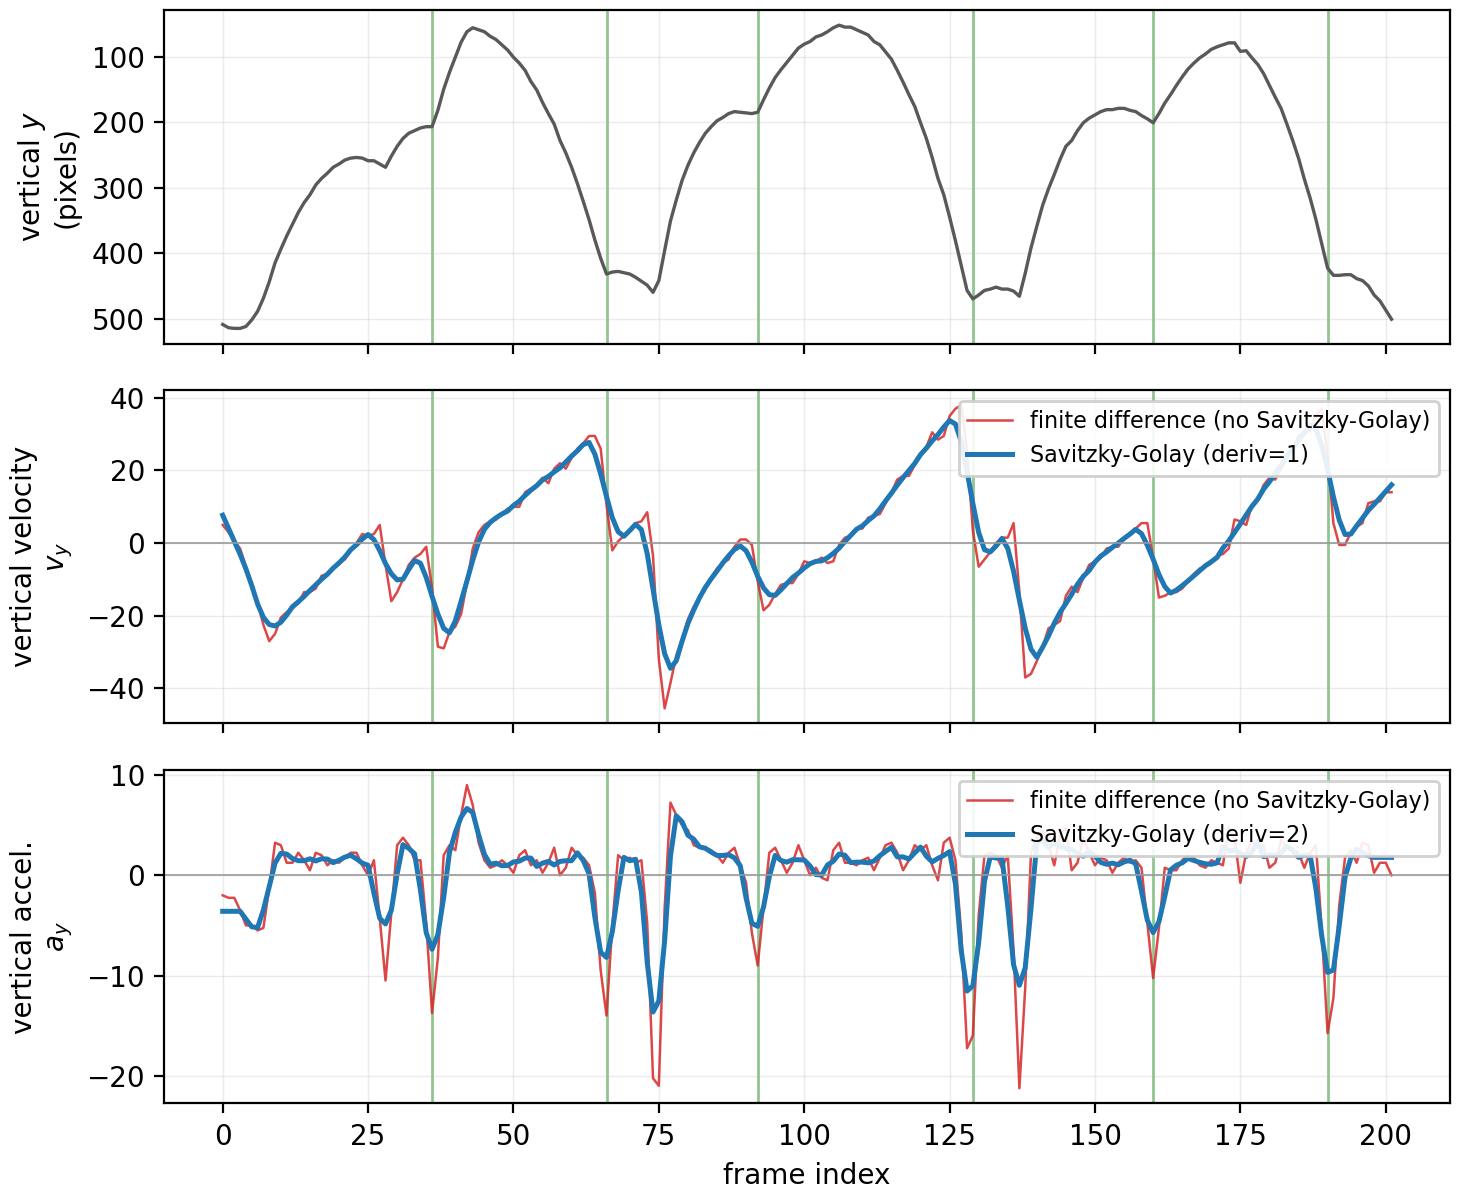
\includegraphics[width=\linewidth]{img/savgol_vs_finite_difference.png}
  \caption{Velocity and acceleration recovered from the vertical ball trajectory
    of one rally, comparing a naive finite difference (red) with the
    Savitzky-Golay smoothing-differentiation filter (blue). Top: the vertical image
    coordinate $y$ against the frame index, with bounce frames marked in green.
    Middle: the first derivative $v_y$. Bottom: the second derivative $a_y$. The
    finite difference amplifies the per-frame jitter in the tracked positions, most
    severely in the acceleration, while the Savitzky-Golay estimate keeps the
    reversal at each bounce and rejects the noise.}
  \label{fig:savgol-vs-finite-difference}
\end{figure}

From this cleaned and differentiated trajectory, two feature representations are
derived, one for each kind of model. For the gradient-boosted model, which sees one frame at a
time, each frame is described by a seventy-one-dimensional vector: eleven base
quantities, namely the normalised position, the velocity and acceleration
components, the speed and acceleration magnitude, the change in heading, the
visibility, and the interpolation flag, together with sixty lag features that
encode the local shape of the trajectory. The lag features compare each frame with
its neighbours up to ten frames away in both directions, as signed vertical
differences, absolute horizontal differences, and, most importantly, the
scale-invariant ratios of the forward to the backward difference. These ratios are
the principal discriminative feature: in free flight the trajectory is locally
monotonic and the ratio of forward to backward motion is close to $-1$, whereas at
a bounce the motion reverses and the ratio flips towards $+1$. For the temporal convolutional network, which sees
a window of frames at once and can learn such lag structure internally, each frame
is described by only seven channels: the normalised position, the velocity and
acceleration components, and the visibility.

The learning target is common to both learned models and is a soft one. Rather
than a single positive frame per bounce, which would make an off-by-one prediction
count as a complete miss and would offer almost no gradient on the scarce positive
class, the target is a Gaussian bump in time of unit peak and a standard deviation
of $1.5$ frames, centred on each bounce frame. Hits and ordinary in-flight frames
carry a target of zero, so that the soft label rewards a prediction near a true
bounce in proportion to its temporal closeness while still treating hits as
negatives.

\section{Models}
\label{sec:bounce-models}

Two models are compared, each mapping a clip's trajectory to a per-frame bounce
score in $[0, 1]$ that the shared decoder of Section~\ref{sec:bounce-decode} turns
into discrete events. Both are learned models that draw the bounce-against-hit
distinction the task demands, but they differ in how much of the trajectory shape
is supplied to them and how much they must learn. The gradient-boosted classifier
is handed an explicit per-frame description of the local trajectory shape, while
the temporal convolutional network is given only the raw per-frame channels and
must learn that shape for itself. This contrast, between an engineered-feature model
and an end-to-end temporal one, is the comparison RQ3 needs.
Table~\ref{tab:bounce-models} summarises them.

\begin{table}[t]
  \centering
  \small
  \setlength{\tabcolsep}{5pt}
  \caption{The two bounce-detection models. The input column distinguishes
    the per-frame model from the windowed one; the trained-parameters column
    counts only learned weights, excluding the single decode threshold that both
    calibrate on the validation split.}
  \label{tab:bounce-models}
  \begin{tabular}{@{}l p{3.0cm} p{3.1cm} l@{}}
    \toprule
    Approach & Input per prediction & Discriminative mechanism & Trained params \\
    \midrule
    XGBoost & one frame, 71 features & boosted regression trees & 515 trees ($\le\!10^3$) \\
    TCN & 64-frame window, 7 channels & dilated temporal convolutions & 10{,}433 weights \\
    \bottomrule
  \end{tabular}
\end{table}


The gradient-boosted model is an ensemble of regression trees, in the gradient
boosting framework of Friedman~\cite{friedman2001gbm}, that maps the
seventy-one-dimensional per-frame feature vector of Section~\ref{sec:bounce-features}
to the soft bounce target. The implementation is XGBoost~\cite{chen2016xgboost}, gradient-boosting model that fits each new tree to the second-order
expansion of a regularised objective and searches for its splits over histogram bins
of the features, so that training over the full per-frame table is both efficient and
resistant to overfitting. It is trained to minimise the squared error against the
soft target, with the frames near a bounce up-weighted so that the scarce positive
region is not drowned out by the negative class, for up to a thousand boosting
iterations with early stopping on a held-out validation split.


The temporal convolutional network processes a window of sixty-four consecutive
frames of the seven-channel representation and emits a bounce logit for every frame
in the window, in the style of temporal convolutional models for sequence
labelling~\cite{lea2017tcn,bai2018tcn}. It is a small stack of four residual
blocks of dilated one-dimensional convolutions, with the dilation doubling from one
block to the next so that the receptive field grows exponentially and a single
output frame can attend to its wider temporal neighbourhood, the same mechanism
that lets dilated convolutions model long-range structure in sequence
data~\cite{vandenoord2016wavenet}. The network is kept deliberately small, only
10{,}433 weights in the configuration used here, because the positive class is
scarce and a larger model would overfit the few hundred training bounces. It is
trained with the
Adam optimiser~\cite{kingma2015adam} against the soft target under a masked focal
binary cross-entropy loss that down-weights the easy negative frames and up-weights
the rare positives, with the loss masked out on the invalid frames identified by
the cleaning step. At inference the network is run over overlapping windows whose
predictions are averaged back into a single per-frame score for the clip. Unlike
the gradient-boosted model it learns its own temporal features from the raw
channels, at the cost of a training loop, and a hardware accelerator to train on.
\section{Decoding and Event Matching}
\label{sec:bounce-decode}

To keep the comparison fair, the per-frame scores of both models pass through
one shared decoder, so that any difference in the reported
events is a difference between the scores and not between the post-processing. The
decoder locates the peaks of the score signal that exceed the model's threshold, subject to a minimum spacing of five frames between successive peaks so
that a single bounce is not reported twice, and treats each surviving peak as one
predicted bounce event; frames masked invalid by the cleaning step are excluded
from the search. The predicted events are then matched to the ground-truth bounce
frames by the greedy one-to-one assignment within $\pm k$ frames defined in
Section~\ref{sec:meth-metrics-event}, closest pair first, from which the true
positives, false positives, and false negatives, and hence the event precision,
recall, and $F_1$ at tolerance $k$, follow. The default tolerance is $k = 3$
frames, and a sweep over $k \in \{0, 1, 2, 3, 5, 7\}$ reports how the score
tightens or relaxes with the timing requirement.

\section{Results}
\label{sec:bounce-results}

The models were evaluated on the game7 test split, a single held-out match
of 1\,881 frames in nine clips containing 50 bounce events
(Table~\ref{tab:splits}). Each model's decode threshold was the value calibrated on
the validation split. Table~\ref{tab:bounce-results} reports the event metrics at
the default tolerance together with the average precision and the event counts, for
the four boosting libraries and the temporal network, and
Figure~\ref{fig:bounce-comparison} plots the tolerance sweep and the
precision-recall curves for the selected XGBoost model against the network.

\begin{table}[t]
  \centering
  \footnotesize
  \setlength{\tabcolsep}{4pt}
  \caption{Bounce-detection results on the game7 test split (50 bounce events), at
    the default tolerance $k = 3$ frames. $P$, $R$, and $F_1$ are the event
    precision, recall, and $F_1$ at that tolerance; AP is the average precision over
    the threshold sweep; TP, FP, and FN are the event counts. Bold marks the best
    value in each column.}
  \label{tab:bounce-results}
  \begin{tabular}{l r r r r r r r r}
    \toprule
    Model & $F_1$ & $P$ & $R$ & AP & TP & FP & FN & FPS \\
    \midrule
    \textbf{XGBoost} & 0.948 & \textbf{0.979} & 0.920 & 0.930 & 46 & \textbf{1} & 4 & \textbf{36{,}045} \\
    HistGBM          & \textbf{0.951} & 0.925 & \textbf{0.980} & 0.874 & 49 & 4 & \textbf{1} & 23{,}211 \\
    LightGBM         & \textbf{0.951} & 0.925 & \textbf{0.980} & 0.866 & 49 & 4 & \textbf{1} & 30{,}610 \\
    CatBoost         & \textbf{0.951} & 0.925 & \textbf{0.980} & 0.771 & 49 & 4 & \textbf{1} & 34{,}910 \\
    \midrule
    TCN              & 0.925 & 0.875 & \textbf{0.980} & \textbf{0.972} & 49 & 7 & \textbf{1} & 1{,}788 \\
    \bottomrule
  \end{tabular}
\end{table}

\begin{figure}[t]
  \centering
  \begin{subfigure}{0.49\textwidth}
    \centering
    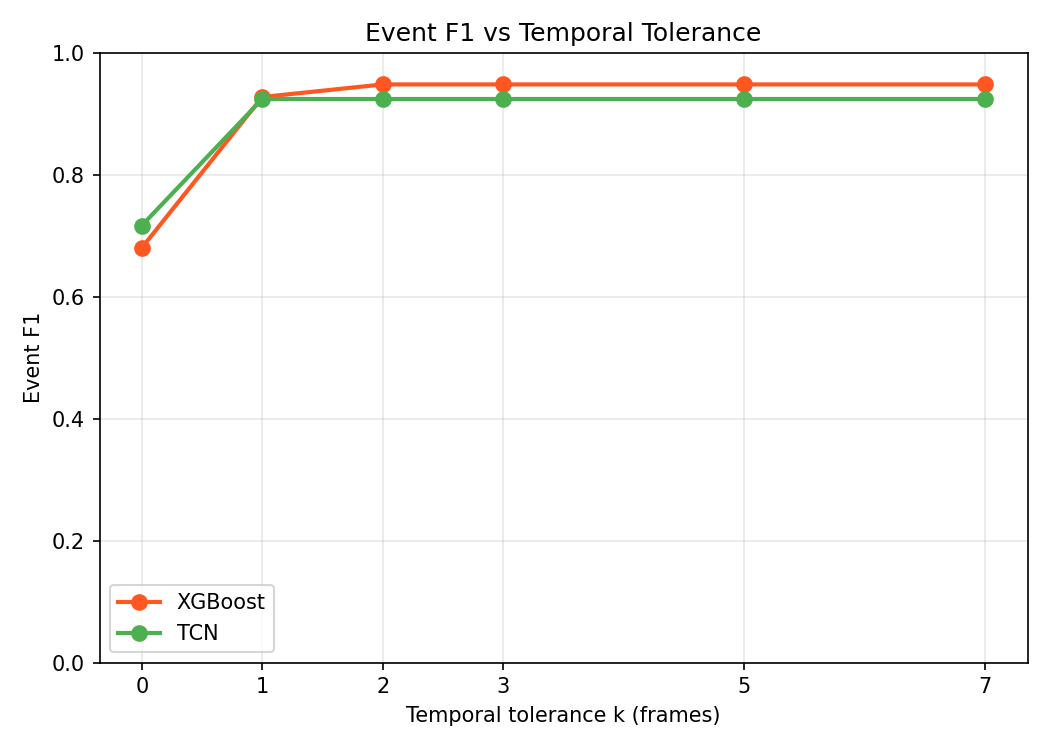
\includegraphics[width=\linewidth]{img/bounce_f1_vs_tolerance.png}
    \caption{$F_1$ across the tolerance sweep.}
    \label{fig:bounce-f1k}
  \end{subfigure}\hfill
  \begin{subfigure}{0.49\textwidth}
    \centering
    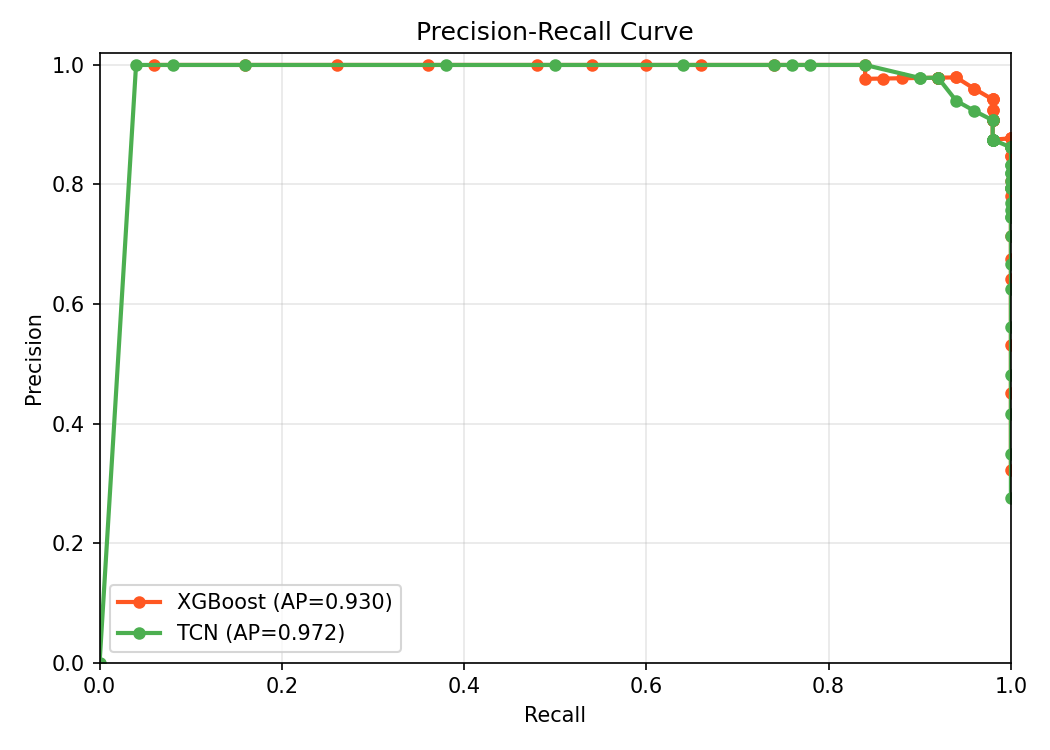
\includegraphics[width=\linewidth]{img/bounce_pr_curve.png}
    \caption{Precision-recall curves.}
    \label{fig:bounce-pr}
  \end{subfigure}
  \caption{Bounce-detection comparison on the game7 test split, for the selected
    XGBoost model against the temporal network. (a)~Event $F_1$ as the matching
    tolerance $k$ widens from $0$ (exact frame) to $7$ frames. At the exact frame the
    temporal network achieves the higher $F_1$ (0.717 against XGBoost's 0.680), but
    from $k = 2$ onward XGBoost leads, and both models plateau by $k = 2$. (b)~The
    precision-recall curves traced by sweeping the decode threshold, whose areas are
    the average precisions of Table~\ref{tab:bounce-results}: the temporal network
    encloses the larger area (AP 0.972 against 0.930).}
  \label{fig:bounce-comparison}
\end{figure}

The four boosting libraries are, for practical purposes, the same model. Their
event $F_1$ spans 0.948 to 0.951, and three of them, the histogram regressor of
scikit-learn, LightGBM, and CatBoost, return the identical confusion of 49 recovered
bounces, four false positives, and one miss; only XGBoost departs from it, and only
at its operating point. What separates the four is not their $F_1$ but the quality of
their score ranking, which the average precision measures: XGBoost reaches 0.930,
well clear of the 0.874, 0.866, and 0.771 of the histogram model, LightGBM, and
CatBoost, so it is the least sensitive of the four to where the decode threshold is
placed. On that robustness, together with its operating-point precision, XGBoost is
the gradient-boosted model carried forward, and the comparison that follows is
between it and the temporal network.

Against the network the two models solve the task about equally well but trade their
errors differently. At the default tolerance XGBoost attains the higher event $F_1$,
0.948 against 0.925,and it raises a single
false positive across the whole test match, for a precision of 0.979, where the
network raises seven, for 0.875. It pays for that caution in recall, recovering 46 of
the 50 bounces against the network's 49, so the network is the more complete detector
and XGBoost the more conservative one. The contrast is the familiar one between a
precision-favouring and a recall-favouring operating point rather than a gap in
capability.

The two lead on different measures, and the swap is informative rather than
contradictory. On the average precision, which integrates over all decode thresholds
and so measures the quality of the score ranking independently of any one operating
point, the temporal network is ahead, at 0.972 against 0.930. On the exact-frame
tolerance $k = 0$ in Figure~\ref{fig:bounce-f1k} it is again ahead, at 0.717 against
0.680, which says it places the peak on the true bounce frame more often; from
$k = 2$ onward, XGBoost takes the lead on
$F_1$ and both plateau. As Section~\ref{sec:meth-metrics-event} cautions, the average
precision and the $F_1$ at a tolerance are different quantities at different operating
points, and on a test set of only fifty events a few false positives or a few missed
bounces are enough to separate two otherwise closely matched models. The fair summary
is that the temporal network has the better score ranking, exact-frame timing, and
recall, while XGBoost is the more precise at the deployed threshold.

These results answer RQ3. Both models solve the timing problem well, each
exceeding an $F_1$ of 0.92 and almost never mistaking a hit for a bounce, which
confirms that learning the trajectory shape succeeds where reading the reversal
alone could not. Between the two the difference is small and direction-dependent,
the temporal network holding the better average precision, exact-frame timing, and
recall, and XGBoost the better $F_1$ and precision. The
engineering costs that separate them, and the consequences of the
ground-truth-trajectory ceiling, are the subject of the analysis below and inform
the model carried into the integrated system of Chapter~\ref{ch:integrated}.

\section{Analysis}
\label{sec:bounce-analysis}

The finding is that the bounce signature is learnable but not reducible to a
simple rule. The cues that mark a bounce, the local maximum of the vertical
position, the velocity sign flip, and the acceleration spike, are genuinely present
at every bounce, but they are equally present at racket hits and at the apex of
every flight, so a detector that thresholds those cues directly cannot resolve the
ambiguity, as Section~\ref{sec:bounce-task} argued from the trajectory itself. Both
learned models succeed on exactly this hit-against-bounce distinction, because they
exploit the finer differences in trajectory shape around the two kinds of event
rather than responding to the reversal alone, and their near-perfect separation of
the two classes confirms that the discriminative information lies in that shape.
This parallels the finding of Chapter~\ref{ch:ball} that a learned localiser
outperforms a geometric one.

Two further caveats qualify the numbers. First, the test set is a single held-out
match with only fifty bounce events, in keeping with the scope noted in
Section~\ref{sec:intro-scope}, so each event is worth two points of recall and a
difference of a few false positives moves the $F_1$ by several points; the gap
between the two learned models in particular should not be over-read, and the
per-game breakdown collapses to this one match. Second, the location of each bounce
in court metres, which the integrated system uses for its line call, is not scored
anywhere in this chapter, because the TrackNet dataset carries no court-keypoint
ground truth and so no in-or-out label against which a projected bounce position
could be checked; the court projection of a detected bounce is therefore a
qualitative capability of the integrated system, taken up in
Chapter~\ref{ch:integrated}, and not a measured result.

In summary, the bounce sub-task answers RQ3 as follows. Separating bounces from the
racket hits that share their kinematic signature calls for a model of the
trajectory shape, not a rule on the reversal. A gradient-boosted model and a small
temporal convolutional network draw that distinction about equally well, and XGBoost, the strongest of the four boosting libraries
tried, is preferred for the integrated system on the strength of its operating-point
precision and its markedly simpler deployment.
\chapter{Integrated System}
\label{ch:integrated}

The three previous chapters each solved one perception sub-task in isolation, on
its own data and against its own metric: locating the ball in every frame
(Chapter~\ref{ch:ball}), registering the playing surface
(Chapter~\ref{ch:court}), and timing the bounces along the resulting trajectory
(Chapter~\ref{ch:bounce}). This chapter combines the three selected models into a
single system that ingests a raw clip and emits one annotated video, and it adds
the step that motivates the whole system: projecting each bounce onto the court
through the estimated homography and deciding, by polygon containment, whether the
ball landed in or out. That composition is the subject of the fourth research
question (RQ4) of Section~\ref{sec:intro-objectives}: whether the best models of
the three sub-tasks can be wired into one end-to-end pipeline that produces tracked
ball, court geometry, bounce events, and a per-bounce line call. The line call is
presented here as a qualitative geometric capability, for the reason developed in
Section~\ref{sec:int-inout} and already flagged in Section~\ref{sec:bounce-analysis}:
the datasets carry no ground-truth in-or-out labels against which it could be
scored.

\section{Architecture}
\label{sec:int-arch}

The integrated system is an orchestration layer over the three component
models. A single entry point reads a video, runs the three models in turn, performs the line-call
geometry, and writes an annotated MP4 together with a summary record.
Figure~\ref{fig:int-pipeline} shows the data flow. The three perception modules are
not retrained or modified here; each is loaded from the checkpoint selected in its
own chapter and wrapped behind a uniform inference call, so that the integration
concerns only how their outputs are combined.

\begin{figure}[t]
  \centering
  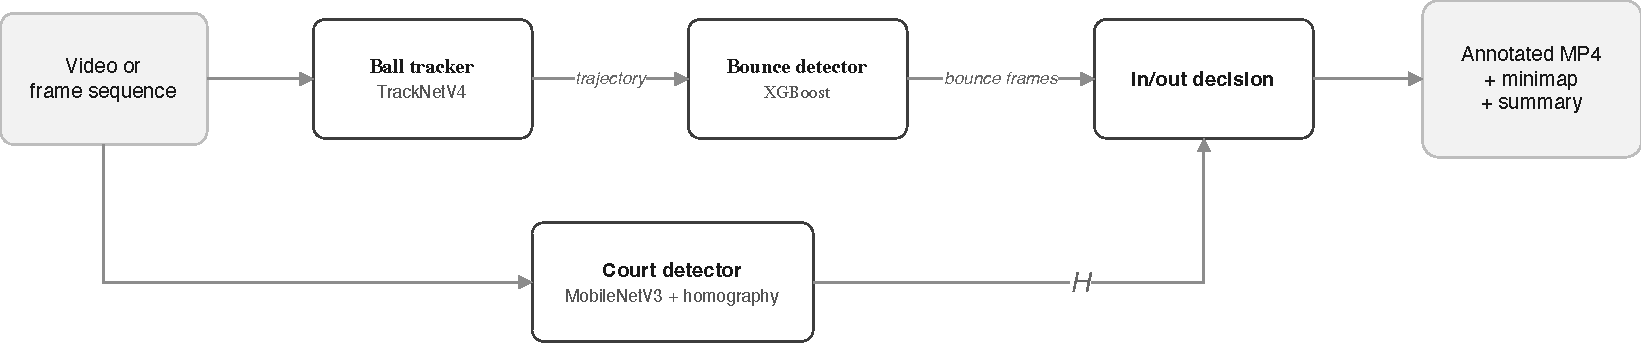
\includegraphics[width=\linewidth]{img/integrated_pipeline.pdf}
  \caption{Data flow of the integrated pipeline. The ball tracker and the court
    detector both consume the input frames; the ball tracker yields a per-frame
    trajectory and the court detector yields a frame-pixel-to-court-metre
    homography $H$. The bounce detector marks bounce frames along the trajectory,
    and the in/out stage projects the ball's position at each bounce through $H$ and
    tests court-polygon containment. All outputs are composited into one annotated
    video with a top-down court minimap and a summary record.}
  \label{fig:int-pipeline}
\end{figure}

The pipeline runs the models in a fixed order, each stage consuming the previous
output. The ball tracker is run first over every frame, producing the trajectory in
its native $640 \times 368$ working resolution, which is then scaled to the
original frame size. The court detector is run on the opening frames
until one yields a valid homography: its keypoints, predicted in a $640 \times 360$
space, are scaled to the original frame size and passed to the RANSAC homography fit
of Section~\ref{sec:court-homography}, and the first frame that produces a usable
$H$ fixes the court geometry for the clip. The bounce detector then runs on the scaled trajectory, and
finally the line-call stage of Section~\ref{sec:int-inout} consumes the trajectory,
the homography, and the detected bounce frames together. The orchestrator returns a
summary record reporting the number of bounces, the in and out counts, the line-call
quality flag, and the measured throughput of the ball and court stages.

\section{In/Out Line Call}
\label{sec:int-inout}

The line call is the step that turns three streams of perception output into the
decision the system is named for. It rests on the homography $H$ of
Section~\ref{sec:court-homography}, which maps a point in frame pixels to its
position on the court in metres. For each detected bounce at which the ball is
visible, the pipeline takes the ball's frame-pixel position at that frame and
projects it through $H$ to a court-metre coordinate, then tests whether that point
lies inside the court polygon. The polygon is the singles or the doubles court, a
choice exposed to the user, expressed as four corner coordinates in the same
court-metre frame as $H$. A bounce that projects inside the polygon is labelled
IN, one outside is labelled OUT.


The honesty of this output must be stated as carefully as its mechanism, and the
qualification is the same one raised in Section~\ref{sec:bounce-analysis}. The line
call is a geometric demonstration, not a validated measurement. Neither dataset of
this thesis carries a ground-truth in-or-out annotation, so there is no label against
which a projected call could be scored, and no accuracy, precision, or error rate for
the line call is reported anywhere in this work.

\section{End-to-End Demonstration}
\label{sec:int-demo}

The complete pipeline was run on a held-out clip from match game10, the same test
match as the ball tracker's final evaluation (Section~\ref{sec:ball-final}), to
exercise every stage on data no component had trained on.
Figure~\ref{fig:int-demo} shows a representative annotated frame. The ball trail, the
IN banner, the expanding ring at the detected bounce, and the court minimap
with its projected trajectory and bounce markers are all visible together, which is
the qualitative evidence that the composition of Section~\ref{sec:int-arch} works
end to end: the trajectory from TrackNetV4, the homography from MobileNetV3, and the
bounce timing from XGBoost combine into a single coherent annotation, and the
homography projection places the bounces sensibly within the court on the minimap.

\begin{figure}[t]
  \centering
  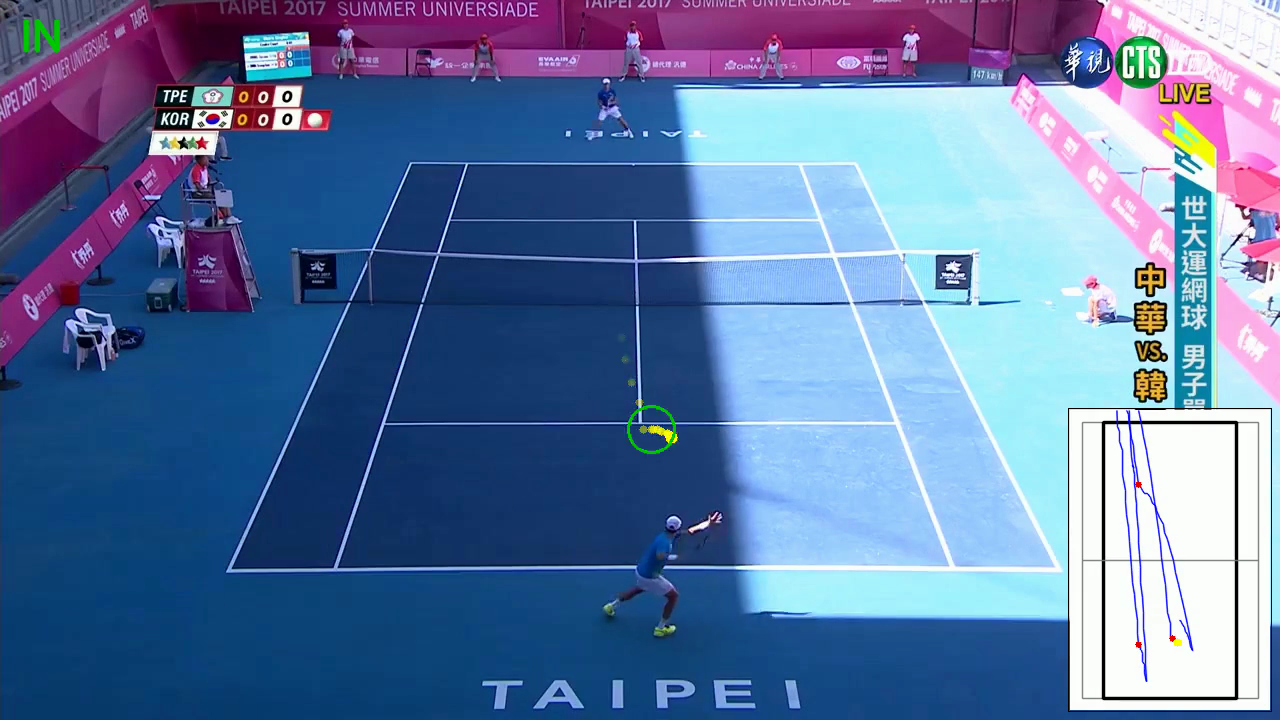
\includegraphics[width=\linewidth]{img/integrated_demo_frame.png}
  \caption{A representative frame from the end-to-end demonstration on a game10 test
    clip. The ball is tracked with a fading trail (yellow); a detected bounce is
    marked by an expanding ring on the court and announced by the banner at the top
    left, here IN (green). The court minimap composited into the bottom-right
    corner shows the singles and doubles court lines, the ball trajectory projected
    into court-metre space (blue), the bounce positions accumulated so far (red), and
    the current ball position (yellow). The line call is a qualitative geometric
    output, not a validated measurement (Section~\ref{sec:int-inout}).}
  \label{fig:int-demo}
\end{figure}


This demonstration answers RQ4. The three models selected on their own sub-tasks do
compose into a single program that takes a raw clip and emits a tracked ball, a
registered court, timed bounces, and a per-bounce in-or-out call. The line call, the application that motivates the
system, is realised as a working geometric capability, with the clear and repeated
caveat that it is qualitative: a demonstration of the pipeline's reach, awaiting the
labelled data and uncertainty modelling that quantitative officiating-grade
validation would require.

\chapter{Discussion}
\label{ch:discussion}

The preceding chapters reported four model comparisons in isolation, one per perception sub-task and one for the integrated system. Read together, the four comparisons share a few patterns worth stating directly, and they fail in a few places worth stating just as directly.

\section{Cross-Cutting Findings}
\label{sec:disc-findings}

The clearest pattern across the study is that, on both perception problems where a learned model could be set against a more direct geometric or rule-based alternative, the learned model won, and it won for the same underlying reason. For ball localisation (Section~\ref{sec:ball-analysis}), the heatmap formulation of TrackNetV4 was a far stronger localiser than the single-frame bounding-box regression of YOLO11m, which was the weakest model by a wide margin. For bounce detection (Section~\ref{sec:bounce-analysis}), both the gradient-boosted classifier and the temporal convolutional network separated genuine bounces from racket hits almost perfectly, even though a hit and a bounce produce the same vertical trajectory reversal and a naive kinematic rule keyed on that reversal cannot tell them apart. The common thread is that the discriminative information in each case lives in fine spatial or temporal shape rather than in a single cue. A tiny tennis ball spanning a handful of pixels is poorly served by a coarse bounding box, but well served by a dense Gaussian heatmap that the network learns to peak precisely \cite{huang2019tracknet, cheng2023smallobjectsurvey}; a bounce is poorly served by detecting a reversal, but well separated from a hit by the full local shape of the trajectory leading into and out of the contact. In both cases the learned representation captured shape that the simpler formulation discarded.

The second recurring finding is that model capacity was not the deciding factor. What mattered was whether the architecture carried the right inductive bias and produced output at the right resolution. The ball comparison is the sharper example: the V1--V5 progression was not monotone in accuracy, and TrackNetV4, whose lightweight motion-attention module injects an explicit motion prior \cite{raj2025tracknetv4}, outperformed the heavier TrackNetV5, whose learned temporal self-attention was left to discover the same cue from data. A strong, cheap inductive bias beat a general, expensive mechanism asked to learn that bias on its own. The court comparison (Section~\ref{sec:court-analysis}) makes the resolution half of the point: the smallest model considered, a MobileNetV3-Small backbone of 1.28 million parameters \cite{howard2019mobilenetv3}, was simultaneously the most accurate at strict tolerance and the fastest, while the two larger stride-four backbones were quantisation-limited and only became competitive once the tolerance was relaxed. Strict-tolerance accuracy there was governed by the heatmap output stride, not by the parameter count of the encoder. Taken together, the ball and court results support one claim: on these problems architectural fit to the task, the correct prior beats raw scale.

\section{Threats to Validity and Limitations}
\label{sec:disc-limitations}

Several factors bound how far these conclusions should be carried. The most concerning is test-set size, which is most acute for bounce detection. The held-out test was a single match (game7) of 1881 frames containing only 50 bounce events. At that scale each individual event is worth roughly two points of recall, and a handful of false positives moves event F1 by several points.

A second limitation concerns latency. The measured per-frame CPU latency of the composed pipeline does not support a real-time claim, and the integrated system is positioned accordingly as an offline analysis tool rather than a live one.

A third and qualitative limitation concerns the in/out line call produced by the integrated system (Section~\ref{sec:int-inout}). That call projects each visible bounce through the court homography into court-metre coordinates and tests polygon containment, but it is reported without any accuracy, precision, or error figure. No dataset carries ground-truth in/out labels against which it could be scored. The output should therefore be read as a plausible visual indication rather than an adjudication.

A fourth limitation is internal to the integrated pipeline. The bounce detector was scored in Chapter~\ref{ch:bounce} on the ground-truth ball trajectory, but in the assembled system (Section~\ref{sec:int-arch}) it consumes the TrackNetV4 trajectory instead. That predicted trajectory carries localisation error which, as the per-visibility breakdown showed, is largest precisely on the occluded near-ground frames where bounces occur. Deployed bounce timing therefore sits below the Chapter~\ref{ch:bounce} numbers by an amount this study did not isolate, and the reported bounce metrics should be read as an upper bound on end-to-end performance rather than a deployed figure.

Finally, the study deliberately omitted several capabilities that a complete match-analysis system would require: there is no player tracking, no pose estimation, no shot classification, no multi-camera fusion, and no 3D reconstruction. These omissions are scope choices rather than oversights, but they mean the system addresses only the ball, court, and bounce perception layer. Collectively, the limitations above motivate the future work outlined in Chapter~\ref{ch:conclusion}.

\chapter{Conclusion and Future Work}
\label{ch:conclusion}

\section{Summary and Answers to the Research Questions}
\label{sec:concl-summary}

A monocular tennis line-calling system has to solve three perception sub-tasks, and this thesis studied each under one deterministic, like-for-like protocol. The hardest is tracking a small, fast ball that often spans only a handful of pixels. Locating the court is more forgiving, and it is what lets image coordinates be tied to the playing surface. The third sub-task, detecting when and where the ball bounces, is what ultimately drives the line call. Rather than proposing a single new architecture, the work framed each sub-task as a controlled comparison between candidate models trained and evaluated on a shared pipeline, and then composed the strongest candidate from each sub-task into one integrated program that produces a per-bounce in/out line call. The four research questions stated in Section~\ref{sec:intro-objectives} are answered in turn below; numbers are comparable only within a sub-task, because the ball and bounce experiments use the TrackNet tennis dataset while the court experiments use a separate court-keypoint dataset.

On ball tracking (RQ1), the comparison covered TrackNet V1--V5 together with the single-frame detector YOLO11m. TrackNetV4 was selected from the six-model subset comparison (Section~\ref{sec:ball-selection}) and then confirmed on the full split (Section~\ref{sec:ball-final}, Table~\ref{tab:ball-final}), where it reached a game10 test acc@5px of 0.956. It led on strict-tolerance localisation and on trajectory smoothness while remaining competitive in speed. The architectural progression from V1 to V5 was not monotone: the lightweight motion-attention of V4 outperformed the heavier temporal self-attention of V5, and the heatmap formulation shared by the TrackNet family clearly outperformed single-frame bounding-box regression, with YOLO11m the weakest localiser of the set.

On court detection (RQ2), four backbones were compared for 14-keypoint localisation. MobileNetV3-Small paired with a full-resolution decoder gave the best accuracy and latency trade-off (Section~\ref{sec:court-results}, Table~\ref{tab:court-results}): a PCK@7px of 0.992, a mean keypoint error of 2.46 px, a court-plane reprojection error of 7.67 cm, and a homography success rate of 0.999, all with only 1.28 million parameters and the fastest inference of the four. The smallest model was also the most accurate, and strict-tolerance accuracy was governed by the output heatmap resolution rather than by backbone capacity. The result is reliable enough to drive the homography on which the integrated system depends.

On bounce detection (RQ3), a gradient-boosted per-frame classifier (XGBoost) was compared with a temporal convolutional network (TCN) for recovering bounce timing from a noisy trajectory (Section~\ref{sec:bounce-results}, Table~\ref{tab:bounce-results}). Both solved the task well, each reaching an event F1 above 0.92 and almost never confusing a racket hit with a bounce, which a simple kinematic-reversal rule cannot do. They traded errors in a direction-dependent way: the TCN had the higher average precision (0.972 against 0.930), the better exact-frame timing (F1@k=0 of 0.717 against 0.680), and the higher recall, while XGBoost had the better tolerant event F1 (F1@k=3 of 0.948 against 0.925) and the higher precision (a single false positive across the match). The gap is small and rests on only 50 test events, so it should not be read as a decisive ranking. XGBoost was carried into the integrated system for its operating-point precision and its markedly simpler deployment.

On integration (RQ4), the three selected models composed into one end-to-end pipeline (Chapter~\ref{ch:integrated}). TrackNetV4, MobileNetV3, and XGBoost were wired into a single program that ingests a raw clip and emits an annotated video with a court minimap and, for each visible bounce, an in/out call obtained by projecting the bounce point through the homography and testing court-polygon containment (Section~\ref{sec:int-inout}, demonstrated in Section~\ref{sec:int-demo}).

\section{Future Work}
\label{sec:concl-future}

The most consequential gap concerns the line call itself. Because no dataset used in this work carries ground-truth in-or-out labels, the geometric verdict produced by the pipeline could not be scored against officiating-grade truth, and quantitative validation therefore requires collecting and annotating such labels before any accuracy claim can be made.

A second cluster of work concerns geometry and data. Monocular video cannot recover the true three-dimensional position of a bounce, so multi-camera fusion and explicit 3D trajectory reconstruction remain the principled path toward officiating accuracy. In parallel, larger and more varied datasets, spanning more matches, surfaces, camera angles, and broadcast styles, would address the domain-shift and small-test-set limitations of this study, most acutely the 50-event bounce test that underlies the RQ3 comparison. 

Finally, deployment and scope offer further work. The current CPU latency places the system in the offline regime, and real-time GPU serving would be needed to lift it toward live use. Beyond the three sub-tasks studied here, the perception stack could be extended to the player tracking, pose estimation, and shot classification that were deliberately placed out of scope (Section~\ref{sec:intro-scope}), broadening the system from line calling toward fuller match analysis.

\section{Closing Remarks}
\label{sec:concl-closing}

The benchmark isolates the design choices that matter within each sub-task, and the integrated demonstrator shows that the selected models compose into a coherent application. What is still missing is the quantitative-officiating layer: without ground-truth in/out labels the geometric verdict stays qualitative. The methodology and the working pipeline are meant to be reused and built on, not treated as a finished officiating system.


% ========================
% REFERENCES
% ========================
\bibliographystyle{IEEEtran}
\bibliography{references}

\end{document}
